%! TEX program = lualatex
% vim:nospell

\RequirePackage{shellesc} % unified shell-escape interface
\RequirePackage[debrief]{silence}
\RequirePackage[l2tabu, orthodox]{nag}
\documentclass[12pt,a4paper,oneside,openright]{book}

%!TEX root = ../main.tex
% vim:nospell

\directlua{pdf.setminorversion(7)}
\RequirePackage{shellesc} % unified shell-escape interface
\RequirePackage[debrief]{silence}
\RequirePackage[l2tabu, orthodox]{nag}

\RequirePackage{xstring}
\StrBetween{\luatexbanner}{\detokenize{n }}{\detokenize{.0 (}}[\luatexversionused] % obtain luatex version used

\providecommand{\pdfxopts}{a-3b,pdf17} % may use options such as a-1a. a-1b
\immediate\write18{rm \jobname.xmpdata} % comment out for non-*nix systems
\begin{filecontents*}{\jobname.xmpdata}
    \Author{Krishnakumar Gopalakrishnan}
\CopyrightURL{https://creativecommons.org/licenses/by-nc-nd/4.0/}
\Copyright{\textcopyright  2018 by Krishnakumar Gopalakrishnan. The copyright  of  this thesis  rests  with the  author  and is  made available  under a  Creative Commons  Attribution Non-Commercial  No Derivatives licence. Researchers are free to copy,  distribute or transmit the thesis on the condition  that they  attribute  it, that  they  do not  use  it for  commercial purposes and that they  do not alter, transform or build upon  it. For any reuse or redistribution,  researchers must make clear  to others the licence  terms of this work.}
\Creator{LuaTeX \luatexversionused\space and pdfx.sty with options \pdfxopts}
\Subject{Lithium ion batteries \sep Mathematical models \sep Electric vehicles \sep Plug-in electric vehicles \sep Electric vehicle industry \sep Electric vehicles--Batteries \sep Battery management systems \sep Battery charging stations (Electric vehicles) \sep Battery industry \sep electrochemistry \sep Electric batteries \sep Numerical calculations \sep Numerical analysis \sep Chemical processes--Mathematical models \sep Simulation methods \sep Computer simulation \sep Computer modeling \sep battery management systems }
\Keywords{lithium-ion batteries \sep electric vehicles \sep mathematical modelling \sep lithium-ion cell \sep electrochemical cell \sep electrolyte model \sep SPM \sep single particle model \sep layer optimisation \sep pouch cell design \sep layer optimisation \sep pseudo-2d model \sep fast charging \sep mathematical models \sep computer simulation }
\pdfxSetCMYKcolorProfileDir{icc_profiles/coated_FOGRA39L_argl.icc}
\pdfxSetRGBcolorProfileDir{icc_profiles/sRGB_IEC61966-2-1_black_scaled.icc}
\Producer{LuaTeX \luatexversionused\space and pdfx.sty with options \pdfxopts}
\PublicationType{PhD Thesis}
\Publisher{Imperial College London}
\Title{Computational modelling of lithium ion batteries for electric vehicle applications: analysis, design and implementation}


\end{filecontents*}

\PassOptionsToPackage{\pdfxopts}{pdfx}
\PassOptionsToPackage{table}{xcolor}
\PassOptionsToPackage{luatex}{pdflscape}
\PassOptionsToPackage{pdfa}{hyperref}

% Options to these packages are passed to them whenever they get loaded
\PassOptionsToPackage{title, titletoc}{appendix}
\PassOptionsToPackage{makeroom}{cancel}
\PassOptionsToPackage{backend=biber, style=numeric-comp, sorting=none, citestyle=numeric-comp, maxbibnames=50, url=true, doi=true, eprint=false, backref=true, backrefstyle=three}{biblatex}
\PassOptionsToPackage{margin=10pt, font=small, labelfont={bf}, labelsep=quad}{caption}
\PassOptionsToPackage{type={CC}, modifier={by-nc-nd}, version={4.0}}{doclicense}
\PassOptionsToPackage{normal}{engord}
\PassOptionsToPackage{inline}{enumitem}
\PassOptionsToPackage{draft}{fixme}
\PassOptionsToPackage{bottom}{footmisc}
\PassOptionsToPackage{luatex, paper=a4paper, hmarginratio=1:1, vmarginratio=1:1, scale=0.75}{geometry}
\PassOptionsToPackage{local, markifdraft}{gitinfo2}
\PassOptionsToPackage{frac, vfrac, multskip}{mathfixs}
\PassOptionsToPackage{section}{placeins}
\PassOptionsToPackage{separate-uncertainty = true, multi-part-units=single, detect-all}{siunitx}
\PassOptionsToPackage{nottoc}{tocbibind}
\PassOptionsToPackage{normalem}{ulem}
\PassOptionsToPackage{no-math, quiet}{fontspec}
\PassOptionsToPackage{warnings-off={mathtools-colon}}{unicode-math}
\PassOptionsToPackage{british}{babel}
\PassOptionsToPackage{final, activate={true, nocompatibility}, factor=1100, stretch=10, shrink=10, babel=true}{microtype}
\PassOptionsToPackage{british}{selnolig}
\PassOptionsToPackage{newfloat=true}{minted}
\PassOptionsToPackage{minted, most}{tcolorbox}
\PassOptionsToPackage{all}{hypcap}
\PassOptionsToPackage{nomain, acronym, xindy}{glossaries-extra}
\PassOptionsToPackage{depth=4, open=true, openlevel=0, numbered=true}{bookmark}
% \PassOptionsToPackage{nameinlink}{cleveref}
\PassOptionsToPackage{hyphenation, lastparline, nosingleletter}{impnattypo}
\PassOptionsToPackage{defaultlines=2, all}{nowidow}

\documentclass[12pt,a4paper,oneside,openright]{book} % using the book document class

%%%%%%%%%% list of packages to be loaded %%%%%%%%%%

% uncommment any commented packages before final submission
\usepackage{afterpage}
\usepackage{algpseudocode}  % http://ctan.org/pkg/algorithmicx
\usepackage{bigints}
\usepackage{cancel}
\usepackage{pdfpages}
\usepackage{tabstackengine} % stackmath macro uses this package

%!TEX root = ../main.tex
% vim:nospell

% useful packages for writing any general  draft document with a small subset of
% packages  only for  book/thesis  style  docs and  another  subset of  packages
% applicable only for luatex
% Most notably, microtype is missing here since it needs to be loaded after babel (which is to be loaded after fontspec)

\usepackage{amsmath}
\usepackage{amsfonts}
\usepackage{amssymb}
\usepackage{anyfontsize} % typically for thesis use; fancy chapter font size and shading
\usepackage{appendix}    % add appendices

\usepackage{babel}       % with british, we get OUP hyphenation material for free
\usepackage{biblatex}    % seems to have strong dependence on csquotes?
\usepackage{booktabs}

\usepackage{caption}     % for improved layout of figure captions with extra margin, smaller font than text
\usepackage{checkend}

% \usepackage[datesep=/,useregional]{datetime2}
\usepackage[datesep=/,style=ddmmyyyy]{datetime2}
% \DTMsetdatestyle{en-GB-numeric}
\usepackage{diffcoeff}   % looks pretty useful for any math-oriented document. Leaving it here

\usepackage{engord}      % an alternative is to use the fmtcount package
\usepackage{enumitem}

\usepackage{fancyhdr}    % Define custom header (before hyperref)
\usepackage{fixme}
\usepackage{flafter}
\usepackage{footmisc}    % typically for thesis use;

\usepackage{geometry}
\usepackage{gitinfo2}
\usepackage{graphicx}    % important to load before fontspec

\usepackage{labelschanged}
\usepackage{lualatex-math}

\usepackage{makecell}
\usepackage{mathtools}
\usepackage{mathfixs}
\usepackage{multicol}
\usepackage{multirow}

\usepackage[section]{placeins} % Defines a \FloatBarrier command

% \usepackage{rotating} % defines a sidewaystable environment
% \usepackage{pdflscape}
\usepackage{lscape}
\usepackage{longtable}
\usepackage{setspace} % Define line spacing

\usepackage{siunitx}
\usepackage{subcaption}

\usepackage{titlesec}  % typically for thesis use;
\usepackage{titletoc}  % typically for thesis use;
\usepackage{threeparttable}
\usepackage{tocbibind} % typically for thesis use; correct page numbers for bib in TOC, nottoc suppresses an entry for TOC itself

\usepackage{ulem}

\usepackage{varwidth}

\usepackage{witharrows}

\usepackage{xfrac}
\usepackage{xpatch} % example use; helpful to replace parens with brackets for backreferencing with biblatex

% ---------- unused packages (but potentially useful) ----------
% \usepackage[backend=biber, style=ieee, sortlocale=en_GB, maxbibnames=50, url=true, doi=true, eprint=true ]{biblatex}
% \usepackage{blindtext}
% \usepackage{chkfloat}
% \usepackage{cite} % incompatible with biblatex
% \usepackage{cmdtrack}
% \usepackage{colortbl} % colortbl cannot be used if xcolor is used
% \usepackage{etoolbox} % not really required if using glossaries package, since this package then gets loaded automatically
% \usepackage{fnpct}
% \usepackage{footnote}
% \usepackage{layouts} % helpful for computing textwidth, textheight etc
% \usepackage{lettrine}
% \usepackage{luabibentry}
% \usepackage{makebox}
% \usepackage[activate={true,nocompatibility},final,tracking=true,factor=1100,stretch=10,shrink=10]{microtype}
% \usepackage{nccmath}
% \usepackage{needspace}
% \usepackage{nolbreaks}
% \usepackage[all,warning]{onlyamsmath} % if using Tikz, please include the calc and babel libraries (known incompatibilities)
% \usepackage{blindtext}
% \usepackage{soulutf8}
% \usepackage{subfiles}
% \usepackage{tablefootnote}
% \usepackage{tabularx}
% \usepackage[table]{xcolor} % loaded by pdfx package (if used) cannot explicitly load colortbl package either before or after
% \usepackage{url}

 % a bit specific to luatex; also includes biblatex

\usepackage{unicode-math} % fontspec after graphicx and babel; https://tex.stackexchange.com/questions/188222/problem-with-babel-and-fontspec; no-math option (math-handling is left to unicode-math); silent to suppress all warnings (even in log file)
%!TEX root = ../main.tex
% vim:nospell

\setmainfont{LibertinusSerif}[%
Extension         = .otf,
Path              = ./fonts/,
UprightFont       = *-Regular,
BoldFont          = *-Bold,
ItalicFont        = *-Italic,
BoldItalicFont    = *-BoldItalic,
Numbers           = {Proportional, Lining},
Ligatures         = {TeX, Common, Required},
SmallCapsFeatures = {Letters = SmallCaps},
% Fractions         = On,
Kerning           = {Uppercase, On},
% FontFace       = {sb}{n}{*-Semibold},
% FontFace       = {sb}{it}{*-SemiboldItalic},
]%

\setsansfont{LibertinusSans}[%
Extension         = .otf,
Path              = ./fonts/,
UprightFont       = *-Regular,
BoldFont          = *-Bold,
ItalicFont        = *-Italic,
BoldItalicFont    = *-BoldItalic,
Numbers           = {Proportional, Lining},
Ligatures         = {TeX, Common, Required},
SmallCapsFeatures = {Letters = SmallCaps},
% Fractions         = On,
Kerning           = {Uppercase, On},
]%

% \setmainfont[Numbers={Proportional},Ligatures={TeX, Common%, Historic, Contextual, Rare, Discretionary
% }]{Libertinus Serif}
% \setsansfont{Libertinus Sans}

\setmonofont{Latin Modern Mono}

% % https://tex.stackexchange.com/questions/103379/minionpro-semibold-medium
% \DeclareRobustCommand\sbseries{\fontseries{sb}\selectfont}
% \DeclareTextFontCommand{\textsb}{\sbseries}

\defaultfontfeatures{ Scale = MatchLowercase }
\defaultfontfeatures[\rmfamily]{ Scale = 1}

% \setmathfont[bold-style = ISO]{LibertinusMath-Regular.otf} % https://github.com/libertinus-fonts/libertinus/issues/20
\setmathfont{LibertinusMath-Regular.otf}[%
Path       = ./fonts/,
bold-style = ISO, % https://github.com/libertinus-fonts/libertinus/issues/20
]%

\setmathfont{libertinusmath-bold.otf}[%
Path       = ./fonts/,
bold-style = ISO, % https://github.com/libertinus-fonts/libertinus/issues/20
version    = bold,
]%

% \setmathfont[math-style=upright,range={`e,`i}]{Latin Modern Math}
% \setmathfont[range={\mathunder,\triangleq},Scale=MatchUppercase]{STIX2Math.otf}
\setmathfont[range = {\mathunder,\triangleq,\underbrace},Scale = MatchUppercase]{Latin Modern Math}

 % selection of unicode text and math fonts

\usepackage{ragged2e}  % should be loaded after the body font and size have been established
\usepackage{microtype} % if using option babel=true, babel must be loaded before microtype; microtype must be loaded after font selection (after fontspec)

\usepackage{selnolig}  % luatex package;  should go after loading babel

\usepackage{float} % Loading order is important here https://tex.stackexchange.com/questions/435529/correct-loading-order-of-package-newfloat-along-with-hyperref-and-algorithmic-pa/435597#435597
\usepackage{minted}
\usepackage{tcolorbox}
\usepackage{csquotes}    % The fvextra package is loaded by minted, so you should load minted before csquotes; has a strong dependency with biblatex
\usepackage{chemformula} % uses tikz arrows

%!TEX root = ../main.tex
% vim: nospell

\usepackage{pdfx}
% https://tex.stackexchange.com/questions/449470/pdfx-package-incompatibility-with-bookmark-package-when-using-luatex-engine/449508#449508
\ifluatex
    \pdftrue
\fi

\usepackage{hyperxmp} % comment out if using the pdfx package
% \usepackage{hyperref} % comment out if using the pdfx package

\hypersetup{%
    anchorcolor        = black,
    baseurl            = {http://spiral.imperial.ac.uk/},
    breaklinks         = true,
    citecolor          = [RGB]{0,68,136}, % https://personal.sron.nl/https://personal.sron.nl/pault/#fig:scheme_highcontrastpault/#fig:scheme_highcontrast
    colorlinks         = true,
    final              = true,
    linkcolor          = [RGB]{0,68,136}, % https://personal.sron.nl/https://personal.sron.nl/pault/#fig:scheme_highcontrastpault/#fig:scheme_highcontrast
    linktocpage        = true,
    pdfauthor          = {Krishnakumar Gopalakrishnan},
    pdfauthortitle     = {PhD student},
    pdfapart           = {3},
    pdfborderstyle     = {/S/U/W 1},
    pdfcaptionwriter   = {Krishnakumar Gopalakrishnan},
    pdfcenterwindow    = true,
    pdfcontactaddress  = {Mechanical Engineering Dept, Exhibition Road, City and Guild Building, Imperial College London, South Kensington},
    pdfcontactcity     = {London, United Kingdom},
    pdfcontactcountry  = {United Kingdom},
    pdfcontactemail    = {krishnak at vt dot edu},
    pdfcontactpostcode = {SW7 2AZ},
    pdfcontactregion   = {Greater London},
    pdfcontacturl      = {https://krishnakumarg.gitlab.io, https://www.linkedin.com/in/krishnakumargopalakrishnan},
    pdfcopyright       = {\textcopyright{} 2019 by Krishnakumar Gopalakrishnan. The    copyright    of    this     thesis    rests    with    the    author. Unless   otherwise    indicated,   its    contents   are    licensed   under a   Creative Commons   Attribution-NonCommercial-NoDerivatives  4.0   International  (CC BY-NC-ND 4.0) Licence. Under this licence, you may  copy and redistribute the material in any medium or format on the condition that: you credit the author, do not use it for commercial purposes  and do not distribute  modified versions of the  work. When reusing or sharing this work, ensure you  make the licence terms clear to others by naming  the licence and linking  to the licence text.  Please seek permission from the copyright  holder for uses of  this work that are not  included in this licence or permitted under UK Copyright Law.},
    pdfcreator         = {LaTeX with hyperref},
    pdfdisplaydoctitle = true,
    pdffitwindow       = true,
    pdfkeywords        = {lithium-ion batteries, electric vehicles, mathematical modelling, lithium-ion cell, electrochemical cell, electrolyte model, SPM, single particle model, layer optimisation, pouch cell design, layer optimisation, pseudo-2d model, fast charging, mathematical models, computer simulation},
    pdflang            = {en-GB-oxendict},
    pdflicenseurl      = {https://creativecommons.org/licenses/by-nc-nd/4.0/},
    pdfmetalang        = {en-GB-oxendict},
    pdfproducer        = {LuaTeX-\luatexversionused},
    pdfsource          = {},
    pdfstartview       = {Fit},
    pdfsubject         = {Lithium ion batteries, Mathematical models, Electric vehicles, Plug-in electric vehicles, Electric vehicle industry, Electric vehicles--Batteries, Battery management systems, Battery charging stations (Electric vehicles), Battery industry, electrochemistry, Electric batteries, Numerical calculations, Numerical analysis, Chemical processes--Mathematical models, Simulation methods, Computer simulation, Computer modeling, battery management systems},
    pdftitle           = {Computational modelling of lithium ion batteries for electric vehicle applications: analysis, design and implementation},
    pdftoolbar         = true,
    plainpages         = false,
    pdfencoding        = auto,
    unicode            = true,
    urlcolor           = [RGB]{0,68,136}, % https://personal.sron.nl/https://personal.sron.nl/pault/#fig:scheme_highcontrastpault/#fig:scheme_highcontrast
}%


% ---------- packages to be loaded after hyperref ----------%

\usepackage{nameref}
\usepackage{algorithm} % http://ctan.org/pkg/algorithms
\usepackage{hypcap} % to be loaded after hyperref. fix hyperref links to jump directly to Table or Figure

\usepackage{pdftexcmds} % not required if using pdfx package

\usepackage{glossaries-extra} % should be loaded after hyperref, but before cleveref % consider 'symbols' option

\usepackage{hypdestopt} % seems to have problems with pdfx package?

\usepackage{bookmark} % improves bookmarks handling. % More features and faster updated bookmarks.
\usepackage{cleveref}

% \usepackage{showframe}
% \usepackage[noframe]{showframe}
\newcommand{\blackurl}{\hypersetup{urlcolor=black}}%
\newcommand{\regularurl}{\hypersetup{urlcolor=[RGB]{0,68,136}}}%

  % hyperref, nameref, algoriothm, hypcap, bookmark, glossaries, cleveref, showframe
\usepackage{doclicense}

\usepackage{impnattypo}
\usepackage{nowidow}

%---------- end of package loading ----------%


%---------- begin custom commands ----------%
%!TEX root = ../main.tex
% vim:nospell ft=tex

\definecolor{mintedbg}{rgb}{0.95,0.95,0.95}
\definecolor{imperialraspberry}{RGB}{145,0,72}

\definecolor{imperialbrick}{RGB}{165,25,0}
\definecolor{sepiadvipsnames}{RGB}{99,29,11}
\definecolor{imperialnavy}{RGB}{0,33,71}
% \definecolor{brickreddvipsnames}{RGB}{173,51,38}
% \definecolor{mahoganydvipsnames}{RGB}{161,53,40}

\definecolor{imperialblue}{RGB}{0,62,116}
\definecolor{cbrewerdarkblue}{RGB}{49,130,189}
\definecolor{viridistendarkblue}{RGB}{56,88,140}
\definecolor{viridistwentyblueseven}{RGB}{49,103,142}
\definecolor{viridistwentybluesix}{RGB}{54,91,141}
\definecolor{viridistwentybluefive}{RGB}{60,78,138}
\definecolor{viridistenlighterblue}{RGB}{45,111,142}
\definecolor{imperiallightblue}{RGB}{0,110,175}
\definecolor{imperialnewblue}{RGB}{0,86,146}

\definecolor{imperialdarkgreen}{RGB}{2,137,59}
\definecolor{imperialprocessblue}{RGB}{0,133,202}

\definecolor{imperiallightgray}{RGB}{235,238,238}
\definecolor{cbrewerlightgray}{RGB}{240,240,240}
\definecolor{cbrewerintergray}{RGB}{189,189,189}
\definecolor{imperialcoolgray}{RGB}{157,157,157}

\definecolor{intermediategray}{RGB}{196,196,196}
\definecolor{cbrewerdarkgray}{RGB}{99,99,99}
\definecolor{lightintergray}{RGB}{215,217,217}

%!TEX root = ../main.tex
% vim:nospell ft=tex

\newcommand{\effdelta}{\ensuremath{{\text{eff}_\delta}}}
\newcommand{\effj}{\ensuremath{{\text{eff}_j}}}
\newcommand{\efflambda}{\ensuremath{{\text{eff}_\lambda}}}
\newcommand{\effmu}{\ensuremath{{\text{eff}_\mu}}}
\newcommand{\effn}{\ensuremath{{\text{eff}_n}}}
\newcommand{\effp}{\ensuremath{{\text{eff}_p}}}
\newcommand{\effs}{\ensuremath{{\text{eff}_s}}}
\newcommand{\elambda}{\ensuremath{{\text{e}_\lambda}}}
\newcommand{\eneg}{\ensuremath{\text{e,neg}}}
\newcommand{\ensub}{\ensuremath{\text{e,n}}}
\newcommand{\epos}{\ensuremath{\text{e,pos}}}
\newcommand{\epsub}{\ensuremath{\text{e,p}}}
\newcommand{\essub}{\ensuremath{\text{e,s}}}

\newcommand{\jinnegposordered}{\ensuremath{j  \in  \left(\text{neg, pos}\right)}}
\newcommand{\jinnegpos}{\ensuremath{j  ∈  \left\{\text{neg, pos}\right\}}}
\newcommand{\jinnegseppos}{\ensuremath{j  ∈  \left\{\text{neg, sep, pos}\right\}}}
\newcommand{\jinnsp}{\ensuremath{j  ∈  \left\{\text{n,s,p}\right\}}}
\newcommand{\jinpossepneg}{\ensuremath{j  ∈  \left\{\text{pos, sep, neg}\right\}}}
\newcommand{\jr}{\ensuremath{{\text{r}_j}}}
\newcommand{\lambdainnegpos}{\ensuremath{\lambda  ∈  \left\{\text{neg, pos}\right\}}}
\newcommand{\lambdainnegseppos}{\ensuremath{\lambda  \in  \{\text{neg, sep, pos}\}}}
\newcommand{\lambdar}{\ensuremath{{\text{r}_\lambda}}}
\newcommand{\maxj}{\ensuremath{{100\%_j}}}
\newcommand{\maxneg}{\ensuremath{{100\%_\text{neg}}}}
\newcommand{\maxpos}{\ensuremath{{100\%_\text{pos}}}}
\newcommand{\minj}{\ensuremath{{0\%_j}}}
\newcommand{\minneg}{\ensuremath{{0\%_\text{neg}}}}
\newcommand{\minpos}{\ensuremath{{0\%_\text{pos}}}}
\newcommand{\muinnegseppos}{\ensuremath{\mu  \in  \{\text{neg, sep, pos}\}}}
\newcommand{\negr}{\ensuremath{{\text{r}_\text{neg}}}}
\newcommand{\nj}{\ensuremath{{\text{n}_j}}}
\newcommand{\nneg}{\ensuremath{{\text{n}_\text{neg}}}}
\newcommand{\npos}{\ensuremath{{\text{n}_\text{pos}}}}
\newcommand{\pj}{\ensuremath{{\text{p}_j}}}
\newcommand{\plambda}{\ensuremath{{\text{p}_\lambda}}}
\newcommand{\pneg}{\ensuremath{{\text{p}_\text{neg}}}}
\newcommand{\posr}{\ensuremath{{\text{r}_\text{pos}}}}
\newcommand{\ppos}{\ensuremath{{\text{p}_\text{pos}}}}
\newcommand{\refflambda}{\ensuremath{{\text{r,eff}_\lambda}}}
\newcommand{\sefflambda}{\ensuremath{{\text{s,eff}_\lambda}}}
\newcommand{\sjavg}{\ensuremath{{\text{s,avg}_j}}}
\newcommand{\sjmax}{\ensuremath{{\text{s,max}_j}}}
\newcommand{\sjsurf}{\ensuremath{{\text{s,surf}_j}}}
\newcommand{\sj}{\ensuremath{{\text{s}_j}}}
\newcommand{\slambdamax}{\ensuremath{{\text{s,max}_\lambda}}}
\newcommand{\slambdasurf}{\ensuremath{{\text{s,surf}_\lambda}}}
\newcommand{\slambda}{\ensuremath{{\text{s}_\lambda}}}
\newcommand{\snegmax}{\ensuremath{{\text{s,max}_\text{neg}}}}
\newcommand{\snegmin}{\ensuremath{{\text{s,min}_\text{neg}}}}
\newcommand{\snegsurf}{\ensuremath{{\text{s,surf}_\text{neg}}}}
\newcommand{\sneg}{\ensuremath{\text{s,neg}}}
\newcommand{\snsub}{\ensuremath{\text{s,n}}}
\newcommand{\sposmax}{\ensuremath{{\text{s,max}_\text{pos}}}}
\newcommand{\spossurf}{\ensuremath{{\text{s,surf}_\text{pos}}}}
\newcommand{\spos}{\ensuremath{\text{s,pos}}}
\newcommand{\spsub}{\ensuremath{\text{s,p}}}
\newcommand{\tplus}{\ensuremath{{t^0_\text{+}}}}

%!TEX root = ../main.tex
% vim:nospell ft=tex

% For unbroken lines in algorithmicx/algpseudocode when typesetting display math

% other alternative: https://tex.stackexchange.com/questions/110431/problems-with-vertical-lines-in-algorithmicx?noredirect=1&lq=1
% https://tex.stackexchange.com/questions/301462/why-are-vertical-rules-dashed-sometimes-with-algorithmic-package
%%%%%%%%%% https://tex.stackexchange.com/questions/350399/indentation-scope-lines-broken-in-algpseudocode%%%%%%%%%
\newcommand*{\algrule}[1][\algorithmicindent]{\hspace*{.2em}{\color{cbrewerdarkgray}\vrule\vrule
width 0pt height \baselineskip depth .1618\baselineskip\hspace*{\dimexpr#1-.5em}}}

\makeatletter
\newcount\ALG@printindent@tempcnta
\def\ALG@printindent{%
    \ifnum \theALG@nested>0% is there anything to print
        \ifx\ALG@text\ALG@x@notext% is this an end group without any text?
            % do nothing
    \else
        \unskip
        % draw a rule for each indent level
        \ALG@printindent@tempcnta=1
        \loop
        \algrule[\csname ALG@ind@\the\ALG@printindent@tempcnta\endcsname]%
        \advance \ALG@printindent@tempcnta 1
        \ifnum \ALG@printindent@tempcnta<\numexpr\theALG@nested+1\relax% can't do <=, so add one to RHS and use < instead
            \repeat
        \fi
    \fi
}%
% needs etoolbox, but this should have been already loaded with glossaries
\patchcmd{\ALG@doentity}{\noindent\hskip\ALG@tlm}{\ALG@printindent}{}{\errmessage{failed to patch}}
\makeatother

\AtBeginEnvironment{algorithmic}{\lineskip0pt}
%%%%%%%%%% https://tex.stackexchange.com/questions/350399/indentation-scope-lines-broken-in-algpseudocode%%%%%%%%%


\algnewcommand\algorithmicinput{\textbf{Initialise:}}
\algnewcommand\Initialise{\item[\algorithmicinput]}

\algnewcommand\algorithmicdata{\textbf{User data:}}
\algnewcommand\Userdata{\item[\algorithmicdata]}

\algnewcommand\algorithmicfulllinecomment{\qquad\quad  \scriptsize \textit{Note:}}
\algnewcommand\FullComment{\item[\algorithmicfulllinecomment]}

\makeatletter
\algrenewcommand\ALG@beginalgorithmic{\footnotesize}
\algrenewcommand\algorithmiccomment[2][\footnotesize]{{#1\hfill\(\triangleright\) #2}}
\makeatother

\algblockdefx[NAME]{ISR}{END}%
[2][Unknown]{\textbf{begin} \textproc{Interrupt Service Routine} #1(#2)}%
{\textbf{return} \Comment[\footnotesize]{resume suspended line in \textsc{Main()}}}

\algblockdefx[NAME]{OutputEqn}{EndOutputEqn}%
[2][\textbf{x}]{\textbf{subroutine} \textproc{ComputeCellVoltage}(#2)}%
{\textbf{return} $V_\text{cell}$ \Comment[\footnotesize]{resume suspended line in \textproc{Simulate\gls{spm}}}}

\newsavebox{\algboxA}
\newsavebox{\algboxB}

\makeatletter
\@addtoreset{algorithm}{chapter}% algorithm counter resets every chapter
\makeatother
\renewcommand{\thealgorithm}{\thechapter.\arabic{algorithm}}% Algorithm # is <chapter>.<algorithm>

\providecommand\algorithmname{algorithm}
\captionsetup[ruled]{font=small,labelfont={bf},labelsep=quad}

\newcommand{\tempcaption}{}% stores the caption
\newcommand{\templabel}{}% stores the label

\newenvironment{customalgo}[3][0.7\textwidth]
{%
    \begin{minipage}{#1}
        \begin{algorithm}[H]
            \centering
            \gdef\tempcaption{#2}% store the caption so we can use it later
            \gdef\templabel{#3}% store the label so we can use it later
            \begin{algorithmic}[1]
            }%
            {%
            \end{algorithmic}
            \caption{\tempcaption}% use the stored caption
            \label{\templabel}
        \end{algorithm}
    \end{minipage}
    % \smallskip
}%

% extent of line-spacing in algorithms
\let\Algorithm\algorithm
\renewcommand\algorithm[1][]{\Algorithm[#1]\setstretch{1.2390625}}

% % https://tex.stackexchange.com/questions/64674/coloring-lines-in-an-algorithm
% \makeatletter
% \newcommand{\algcolor}[2]{%
%     \hskip-\ALG@thistlm\colorbox{#1}{\parbox{\dimexpr\linewidth-2\fboxsep}{\hskip\ALG@thistlm\relax #2}}%
% }
% \newcommand{\algemph}[1]{\algcolor{cbrewerintergray}{#1}}
% \makeatother


%  https://tex.stackexchange.com/questions/64674/coloring-lines-in-an-algorithm
\makeatletter
% code borrowed from Andrew Stacey; See
% https://tex.stackexchange.com/a/50054/3954
\tikzset{%
    remember picture with id/.style={%
        remember picture,
        overlay,
        save picture id=#1,
    },
    save picture id/.code={%
        \edef\pgf@temp{#1}%
        \immediate\write\pgfutil@auxout{%
        \noexpand\savepointas{\pgf@temp}{\pgfpictureid}}%
    },
    if picture id/.code args={#1#2#3}{%
        \@ifundefined{save@pt@#1}{%
            \pgfkeysalso{#3}%
            }{
            \pgfkeysalso{#2}%
        }
    }
}

\def\savepointas#1#2{%
    \expandafter\gdef\csname save@pt@#1\endcsname{#2}%
}

\def\tmk@labeldef#1,#2\@nil{%
    \def\tmk@label{#1}%
    \def\tmk@def{#2}%
}

\tikzdeclarecoordinatesystem{pic}{%
    \pgfutil@in@,{#1}%
    \ifpgfutil@in@%
        \tmk@labeldef#1\@nil
    \else
        \tmk@labeldef#1,(0pt,0pt)\@nil
    \fi
    \@ifundefined{save@pt@\tmk@label}{%
        \tikz@scan@one@point\pgfutil@firstofone\tmk@def
        }{%
        \pgfsys@getposition{\csname save@pt@\tmk@label\endcsname}\save@orig@pic%
        \pgfsys@getposition{\pgfpictureid}\save@this@pic%
        \pgf@process{\pgfpointorigin\save@this@pic}%
        \pgf@xa=\pgf@x
        \pgf@ya=\pgf@y
        \pgf@process{\pgfpointorigin\save@orig@pic}%
        \advance\pgf@x by -\pgf@xa
        \advance\pgf@y by -\pgf@ya
    }%
}

\makeatother
% end of Andrew's code

% main command to draw the colored background
\newcounter{mymark}
\newcommand\ColorLine{%
    \stepcounter{mymark}%
    \tikz[remember picture with id=mark-\themymark,overlay] {;}%
    \begin{tikzpicture}[remember picture,overlay]%
        \filldraw[cbrewerintergray]%
            let \p1=(pic cs:mark-\themymark),
            \p2=(current page.east)  in
            ([xshift=-0.1em,yshift=-1.0ex]0,\y1)  rectangle ++([xshift=-2.525cm]\x2,\baselineskip);
    \end{tikzpicture}%
}%



 % for typesetting of algorithms
%!TEX root = ../main.tex
% vim:nospell

% \addbibresource{backmatter/thesis_refs.bib}
\ShellEscape{biber --tool backmatter/thesis_refs.bib} % deduplicate bibtex entries
\addbibresource{backmatter/thesis_refs_bibertool.bib}
\addbibresource{backmatter/thesis_refs_joint.bib}

% https://brianbuccola.com/how-to-cite-in-latex-without-the-citation-appearing-in-the-bibliography/
\DeclareBibliographyCategory{ignore}
\addtocategory{ignore}{Gopalakrishnan2018joint}

\renewcommand*{\bibfont}{\small} % make Bibliography left aligned, not justified

\DeclareSourcemap{
    \maps[datatype=bibtex]{
        \map{
            \step[fieldsource=doi,final]
            \step[fieldset=url,null]
        }
    }
}

\DefineBibliographyStrings{english}{%
    backrefpage = {cited on page},% originally "cited on page"
    backrefpages = {cited on pages},% originally "cited on pages"
}

\xpatchbibmacro{pageref}{parens}{brackets}{}{}   % helpful to replace parens with brackets for backreferencing with biblatex % needs xpatch

% \renewbibmacro*{pageref}{\iflistundef{pageref}{}{\printtext[brackets]{\printlist[​pageref][-\value{listtotal}]{pageref}}}}

\DeclareSourcemap{
    \maps[datatype=bibtex]{
        \map[overwrite]{
            \step[fieldsource=month, match=\regexp{\Ajan\Z}, replace=1]
            \step[fieldsource=month, match=\regexp{\Afeb\Z}, replace=2]
            \step[fieldsource=month, match=\regexp{\Amar\Z}, replace=3]
            \step[fieldsource=month, match=\regexp{\Aapr\Z}, replace=4]
            \step[fieldsource=month, match=\regexp{\Amay\Z}, replace=5]
            \step[fieldsource=month, match=\regexp{\Ajun\Z}, replace=6]
            \step[fieldsource=month, match=\regexp{\Ajul\Z}, replace=7]
            \step[fieldsource=month, match=\regexp{\Aaug\Z}, replace=8]
            \step[fieldsource=month, match=\regexp{\Asep\Z}, replace=9]
            \step[fieldsource=month, match=\regexp{\Aoct\Z}, replace=10]
            \step[fieldsource=month, match=\regexp{\Anov\Z}, replace=11]
            \step[fieldsource=month, match=\regexp{\Adec\Z}, replace=12]
        }
    }
}


% https://tex.stackexchange.com/questions/113039/trying-to-suppress-urls-with-biblatex-using-a-simple-persons-method
% \AtEveryCitekey{\clearfield{url}}

% https://tex.stackexchange.com/questions/46787/is-there-a-way-to-prevent-urls-from-appearing-in-biblatex-citations
\AtEveryCitekey{%
    \clearfield{url}%
    \clearfield{urlyear}%
    \clearfield{doi}%
}%
\renewbibmacro*{in:}{}


% https://tex.stackexchange.com/questions/24979/citing-authors-full-name-in-biblatex
\DeclareCiteCommand*{\citeauthor}
{\defcounter{maxnames}{99}%
    \defcounter{minnames}{99}%
    \defcounter{uniquename}{2}%
    \boolfalse{citetracker}%
    \boolfalse{pagetracker}%
\usebibmacro{prenote}}
{\ifciteindex{\indexnames{labelname}}{}%
    \printnames{labelname}}
    {\multicitedelim}
    {\usebibmacro{postnote}}


% \renewcommand*{\mkbibnamefirst}[1]{\edef\firstname{#1}\expandafter\first{\firstname}}
\renewcommand*{\mkbibnamegiven}[1]{\edef\firstname{#1}\expandafter\first{\firstname}}

\def\bibnamedelima{ }%
\def\bibnamedelimb{ }%

\makeatletter
\def\@empty{}
\def\first#1{\expandafter\@first#1 \@nil}
\def\@first#1 #2\@nil{#1\addspace%
  \if\relax\detokenize{#2}\relax\else\@initials#2\@nil\fi}
\def\initials#1{\expandafter\@initials#1 \@nil}
\def\@initials#1 #2\@nil{%
  \initial{#1}%
  \def\NextName{#2}%
  \ifx\@empty\NextName\relax%
  \else\bibinitdelim \@initials#2\@nil\fi}
\def\initial#1{\expandafter\@initial#1\@nil}
\def\@initial#1#2\@nil{#1\bibinitperiod}
\makeatother


% \makeatletter
% \DeclareCiteCommand{\longfullcite}
% {\usebibmacro{prenote}}
% {\usedriver
%     {\c@maxnames\blx@maxbibnames\relax
%     \DeclareNameAlias{sortname}{default}}
% {\thefield{entrytype}}}
% {\multicitedelim}
% {\usebibmacro{postnote}}
% \makeatother

% \newcommand{\longfullcite}{%
%     \AtNextCite{\defcounter{maxnames}{99}}%
% \fullcite}

\newcommand{\printpublication}[1]{\AtNextCite{\defcounter{maxnames}{99}}\fullcite{#1}}

\DeclareBibliographyAlias{software}{online}

% https://tex.stackexchange.com/questions/468623/indicating-joint-first-authorship-through-special-markup-in-biblatex-biber/468634#468634
\renewcommand*{\mkbibnamefamily}[1]{%
    \ifitemannotation{jointfirst}
        {\uline{\textbf{#1}}}
    {#1}}

\renewcommand*{\mkbibnamegiven}[1]{%
    \ifitemannotation{jointfirst}
        {\uline{\textbf{#1}}}
    {#1}}
     % 'bib' file goes in here
%!TEX root = ../main.tex
% vim:nospell ft=tex

\DeclareGraphicsExtensions{.pdf, .png, .jpg, .jpeg} % GIF doesn't work??

%!TEX root = ../main.tex
% vim:nospell ft=tex

\renewcommand{\CancelColor}{\color{imperialbrick}}
     % uses a predefined color

%!TEX root = ../main.tex
% vim:nospell ft=tex

\DeclareCaptionLabelSeparator{note}{\footnotemark \hspace*{0.5em}}

%!TEX root = ../main.tex
% vim:nospell ft=tex

\crefname{listing}{\MakeLowercase{\listingname}}{\MakeLowercase{\listingname s}}
\crefname{appchap}{appendix}{appendices}
\crefname{filePrg}{listing}{listings}
\Crefname{filePrg}{Listing}{Listings}

\newcommand{\crefrangeconjunction}{--}
\crefrangeformat{equation}{eqs.~(#3#1#4)--(#5#2#6)}


%!TEX root = ../main.tex
% vim:nospell ft=tex

\makeatletter
\newcommand{\monthyeardate}{%
  \DTMenglishmonthname{\@dtm@month} \@dtm@day, \@dtm@year
}
\makeatother

%!TEX root = ../main.tex
% vim:nospell ft=tex

% \diffset[p-delims = . |, p-nudge = 0]

\diffdef { p }
{
    op-symbol = \partial ,
    left-delim = \left .,
    right-delim = \right | ,
    subscr-nudge = 0 mu
}

%!TEX root = ../main.tex
% vim:nospell ft=tex

\setlist[enumerate,itemize,description]{topsep=0em}

\newcounter{descriptcount}
\newlist{enumdescriptnum}{description}{1}
\setlist[enumdescriptnum] {%
    before={\setcounter{descriptcount}{0}%
    \renewcommand*\thedescriptcount{\alph{descriptcount}.}}
    ,font=\footnotesize{\bfseries\stepcounter{descriptcount}\thedescriptcount~}
}


\newcommand{\customenum}[2]{
\item[$ \symbf{#1}\  (\times #2)$]
}


%!TEX root = ../main.tex
% vim:nospell ft=tex

\newcommand{\setFancyHdr}{
    \pagestyle{fancy}
    \renewcommand{\chaptermark}[1]{\markboth{\MakeUppercase{\thechapter. ##1 }}{}}
    \renewcommand{\sectionmark}[1]{\markright{\thesection\ ##1}}
    \fancyhf{}
    \fancyhead[R]{\bfseries\rightmark}
    \fancyfoot[C]{\thepage}
    \fancypagestyle{plain}{
        \fancyhead{}
        \renewcommand{\headrulewidth}{0pt}
    }
}

\setlength{\headheight}{14.5pt}
\setFancyHdr

\renewcommand{\headrulewidth}{\iffloatpage{0pt}{0.4pt}}


%!TEX root = ../main.tex
% vim:nospell ft=tex

\fxsetup{theme=color, marginface=\singlespacing \scriptsize}

\definecolor{fxnote}{RGB}{165,25,0} % imperialbrick (duplicating the color-line here, since `fxnote' is the specific color-name hard-coded by the fxnote package)

%!TEX root = ../main.tex
% vim:nospell ft=tex

% https://tex.stackexchange.com/questions/32819/draw-box-with-colored-background-and-linebreaks-which-adjusts-to-the-text-width
\newcommand\MyCBox[1]{%
      \colorbox{cbrewerfourclssor}{\begin{varwidth}{\dimexpr\linewidth-2\fboxsep}#1\end{varwidth}}}

\renewcommand{\gitMarkFormat}{\color{imperialraspberry} \small}
\renewcommand{\gitMark}{Author: {Krishnakumar Gopalakrishnan}, Imperial College London\, \textbullet{}\, \MyCBox{Confidential (Under Embargo)} \\ Typeset by \StrBehind{\luatexbanner}{\detokenize{This is}}{}  engine using the \LaTeX{} macro format}
\renewcommand{\gitMarkPref}{PhD Thesis}


%!TEX root = ../main.tex
% vim:nospell ft=tex

% \renewcommand*{\glstextformat}[1]{\textsf{#1}}
\renewcommand*{\glstextformat}[1]{\textcolor{black}{#1}} % link coloring to match normal text, ie black
\preto\chapter{\glsresetall} % expand acronyms every chapter https://tex.stackexchange.com/questions/435617/glossaries-expand-acronyms-for-first-time-use-within-each-chapter/435680#435680

% \glsdisablehyper
% \newglossary[slg]{symbolslist}{syi}{syg}{Symbols}

% \newglossarystyle{custom_acronyms}
% {
%     \setglossarystyle{long3colheader}%
%     \renewcommand*{\glossaryheader}{}%
%     \renewcommand{\glossentry}[2]{%
%         \textbf{\glsentryitem{##1}\glstarget{##1}{\glossentryname{##1}}}
%         & \glossentrydesc{##1}
%         & {\hspace*{\fill} ##2}
%     \tabularnewline}%
% }

% \renewcommand{\glossarypreamble}{\footnotesize}
% \renewcommand{\glossarypreamble}{\small}
\setglossarypreamble[acronym]{\small}
\setglossarypreamble[symbols]{\normalsize}
% \renewcommand\glstreepredesc{\qquad}

% https://tex.stackexchange.com/questions/118182/selectively-turn-off-hyperref-links-for-citations
\newcommand*{\nolink}[1]{%
      {\protect\NoHyper#1\protect\endNoHyper}%
  }

\glssetcategoryattribute{acronym}{nohyperfirst}{true} % no hyperlink on first use for entries with category=acronym % https://tex.stackexchange.com/questions/434160/line-break-long-glossaries-entry-when-using-hyperref-and-latex-dvips-ps2pdf
\setabbreviationstyle[acronym]{long-short} % applicable only for glossaries-extra.sty

\GlsXtrLoadResources[
src={frontmatter/acronyms},%
selection={all},
type=acronym,% put these entries in the 'acronym' glossary
save-locations=false% don't save locations
]

% assign titles to group labels:
\glsxtrsetgrouptitle{latin}{List of Latin Symbols}
\glsxtrsetgrouptitle{greek}{List of Greek Symbols}
\glsxtrsetgrouptitle{generic}{Other Generic Nomenclature}

\GlsXtrLoadResources[
src={frontmatter/latin-symbols},
sort={letter-lowerupper},
type=symbols,
selection={all},
category={same as entry},% set the category to the entry type
group={latin},% assign group label
set-widest,% needed for 'alttree' styles
save-locations=false
]

\GlsXtrLoadResources[
src={frontmatter/greek-symbols},% entries in 'greek-symbols.bib'
type=symbols,% put these entries in the 'symbols' glossary
selection={all},
category={same as entry},% set the category to the entry type
group={greek},% assign group label
set-widest,% needed for 'alttree' styles
save-locations=false% don't save locations
]

\GlsXtrLoadResources[
src={frontmatter/generic-symbols},
sort={en-GB},
type=symbols,
selection={all},
category={same as entry},% set the category to the entry type
group={generic},% assign group label
set-widest,% needed for 'alttree' styles
save-locations=false
]

\renewcommand{\glsnamefont}[1]{\textbf{#1}} % to bold-face acronym header with style=super
\glssetcategoryattribute{symbol}{glossdescfont}{normalsize} % https://tex.stackexchange.com/questions/303888/different-formatting-for-acronyms-and-glossary-entries


%!TEX root = ../main.tex
% vim:nospell ft=tex

% https://tex.stackexchange.com/questions/304449/combine-minted-and-tcolorbox-for-code-from-file-inputminted/304691#304691
% https://tex.stackexchange.com/questions/304449/combine-minted-and-tcolorbox-for-code-from-file-inputminted/304975#304975
\newcounter{filePrg}

\newtcbinputlisting[use counter=filePrg,number within=chapter,list inside=mypyg]{\matlabcodelisting}[3][]{%
    listing engine=minted,
    minted language=matlab,
    % minted style=algol_nu, % xcode,emacs, perldoc, pastie, borland, vs, vim, tango
    listing file={#2},
    title=\small{\textbf{Listing \thetcbcounter}\quad {#1}},
    % fonttitle=\bfseries,
    listing only,
    list entry={\protect\numberline{\thetcbcounter} #1},
    enhanced jigsaw,
    breakable,
    % drop fuzzy shadow,
    minted options={
        fontsize=\scriptsize,
        breaklines,
        autogobble,
        linenos,
        numbersep=3mm,
        mathescape,
        baselinestretch=1,
        breakanywhere=true
    },
    % colback=offwhite,
    colback=white,
    colframe=imperialnavy,
    % colframe=black,
    % coltitle=white,
    % boxrule=0.2mm,
    left=5mm,
    overlay={\begin{tcbclipinterior}
            \fill[imperiallightgray] (frame.south west) rectangle ([xshift=5mm]frame.north west);
        \end{tcbclipinterior}
    },
    label=#3
}

\pretocmd{\chapter}{\addtocontents{mypyg}{\addvspace{10pt}}}{}{}

\makeatletter % no indent for entries
\renewcommand{\l@tcolorbox}{\@dottedtocline{1}{0pt}{2.3em}}
\makeatother


\SetupFloatingEnvironment{listing}{name=Code snippet} % needs new float package

%!TEX root = ../main.tex
% vim:nospell ft=tex

\WarningFilter{latex}{Marginpar on page}

%!TEX root = ../main.tex
% vim:nospell ft=tex

\sisetup{
    locale = UK ,
    per-mode = reciprocal-positive-first,
    binary-units = true
}
\sisetup{range-phrase=--}
\sisetup{range-units=single}

\DeclareSIUnit \amphour { Ah }
\DeclareSIUnit \watthour { Wh }

%!TEX root = ../main.tex
% vim:nospell ft=tex

% \titleformat*{\section}{\large\bfseries}
\titleformat{\section}{\normalfont\fontsize{16}{21}\bfseries}{\thesection}{1em}{}


% \titlespacing*{<command>}{<left>}{<before-sep>}{<after-sep>}
% before =  1.4453125 canonical for chapter 2 litt review
% \titlespacing*{\section} {0pt}{1.4453125ex plus 0.7225ex minus 0.7225ex}{0ex}
\titlespacing*{\section}{0pt}{1ex plus 0.5ex minus 0.5ex}{0.22ex plus 0.11ex minus 0.11ex}

\titlespacing*{\subsection}{0pt}{1ex plus 0.5ex minus 0.5ex}{0.22ex plus 0.11ex minus 0.11ex}

\titlespacing*{\subsubsection}{0pt}{0.5ex plus 0.25ex minus 0.25ex}{0.11ex plus 0.055ex minus 0.055ex}


%!TEX root = ../main.tex
% vim:nospell ft=tex

\setlength{\ULdepth}{4.0pt}
\renewcommand{\ULthickness}{0.75pt}


%!TEX root = ../main.tex
% vim:nospell ft=tex

\WithArrowsOptions{displaystyle,tikz={font={\scriptsize}}}


%!TEX root = ../main.tex
% vim:nospell ft=tex


\newcolumntype{P}[1]{>{\RaggedRight\hspace{0pt}}p{#1}}
% \newcolumntype{R}[1]{>{\raggedleft\let\newline\\\arraybackslash\hspace{0pt}}m{#1}}
\newcolumntype{C}[1]{>{\centering\arraybackslash}p{#1}}

\makeatletter

\newcommand*{\@rowstyle}{}

\newcommand*{\rowstyle}[1]{% sets the style of the next row
    \gdef\@rowstyle{#1}%
    \@rowstyle\ignorespaces%
}

\newcolumntype{=}{% resets the row style
    >{\gdef\@rowstyle{}}%
}

\newcolumntype{+}{% adds the current row style to the next column
    >{\@rowstyle}%
}

\makeatother


%!TEX root = ../main.tex
% vim:nospell ft=tex

\usetikzlibrary{calc}
\usetikzlibrary{decorations.pathreplacing}

\newcommand{\tikzmark}[1]{\tikz[overlay,remember picture] \node (#1) {};}

% Tweak these as necessary
\newcommand*{\BraceAmplitude}{0.5em}%
\newcommand*{\BraceAspect}{0.5}%
\newcommand*{\VerticalOffset}{3.0ex}%
\newcommand*{\HorizontalOffset}{0.0em}%


\NewDocumentCommand{\InsertUnderBrace}{%
    O{} % #1 = draw options
    O{} % #2 = optional brace options
    m   % #3 = left tikzmark
    m   % #4 = right tikzmark
    m   % #5 = text to place underbrace
    }{%
    \begin{tikzpicture}[overlay,remember picture]
        \draw [decoration={brace, amplitude=\BraceAmplitude, aspect=\BraceAspect, #2}, decorate, thick, draw=blue, text=black, #1]
            ($(#4)+(\HorizontalOffset,-\VerticalOffset)$) --
            ($(#3)+(-\HorizontalOffset,-\VerticalOffset)$)
            node [below=\VerticalOffset, midway] {#5};
    \end{tikzpicture}%
}%

%!TEX root = ../main.tex
% vim:nospell ft=tex

% these custom commands  are general purpose definitions that are  suitable in a
% typical scientific  document. Some  of them  are pure  latex while  others use
% external packages

%---------- for text and other typographical elements ----------%
\newcommand{\eg}{\textit{e}.\textit{g}.}
\newcommand{\etal}{\textit{et~al}.}
\newcommand{\ie}{\textit{i}.\textit{e}.,}
\newcommand{\viz}{\textit{viz}. }

\def\Vhrulefill{\leavevmode\leaders\hrule height 0.7ex depth \dimexpr0.4pt-0.7ex\hfill\kern0pt}
\newcommand*{\xdash}[1][3em]{\rule[0.5ex]{#1}{0.55pt}}

\setlength\parskip{0.75\baselineskip plus0.1\baselineskip  minus0.1\baselineskip}

% https://tex.stackexchange.com/questions/23487/how-can-i-get-roman-numerals-in-text
\makeatletter
\newcommand*{\romanletter}[1]{\expandafter\@slowromancap\romannumeral #1@}
\makeatother


%---------- inline/display math macros ----------%
\newcommand*\mean[1]{\overline{#1}}

\DeclarePairedDelimiter\abs{\lvert}{\rvert}
\DeclarePairedDelimiter\ceil{\lceil}{\rceil}
\DeclarePairedDelimiter\floor{\lfloor}{\rfloor}

\let\mathbbalt\mathbb  % unicode-math changes mathbb to mathbbalt by default % https://tex.stackexchange.com/questions/360607/unicode-math-but-ordinary-blackboard-bold/360637#360637

% ---------- 'increasing spacing between matrix rows' -------------------- %
% https://tex.stackexchange.com/questions/14071/how-can-i-increase-the-line-spacing-in-a-matrix

% a redefinition of an internal amsmath LaTeX macro for customizing line spacing
% in  specific matrices  arbitrarily  as  desired: After  putting  this in  your
% preamble, you can write \begin{pmatrix}[1.5] vary  the value as you like, with
% pmatrix, vmatrix, bmatrix  and alike, or use it without  the optional argument
% as usually.

\makeatletter
\renewcommand*\env@matrix[1][\arraystretch]{%
    \edef\arraystretch{#1}%
    \hskip -\arraycolsep
    \let\@ifnextchar\new@ifnextchar
\array{*\c@MaxMatrixCols c}}
\makeatother
% ---------- end of 'increasing spacing between matrix rows' -------------------- %

% ---------- 'section/chapter/title/footnote handling' ---------- %

% improved handling of sectioning commands with titlesec
\setcounter{secnumdepth}{3} % organisational level that receives a numbers
\setcounter{tocdepth}{3}    % print table of contents for level 3

% needs the anyfontsize package
\renewcommand{\chaptername}{} % uncomment to print only "1" not "Chapter 1"
\titleformat{\chapter}[display]
{\bfseries\sffamily\Huge}
{\hfill\fontsize{140}{50}\selectfont\color{lightgray}\rmfamily\textbf{\thechapter}}% label
{-0ex}
{\filleft\fontsize{50}{50}}
[\vspace{-0ex}]

% \setlength{\columnsep}{20pt} % space between columns in two column mode; default 10pt quite narrow

\renewcommand{\footnoterule}{%
    \kern -3pt
    \hrule width 0.25\textwidth height 0.5pt
    \kern 2pt
}

\renewcommand{\thefootnote}{\fnsymbol{footnote}}

% ---------- end of 'section/chapter/title/footnote handling' ---------- %


% \newenvironment{mycenter}[1][\topsep]
% {\setlength{\topsep}{#1}\par\kern\topsep\centering}% \begin{mycenter}[<len>]
% {\par\kern\topsep}% \end{mycenter}

% not sure why this is being used
\makeatletter
\global\let\tikz@ensure@dollar@catcode=\relax
\makeatother

% To continue roman numbering at the end of the book (for bibliography, appendices etc.)

% \makeatletter
% \newcounter{savepagenumber}
% \renewcommand\mainmatter{%
%     \cleardoublepage
%     \setcounter{savepagenumber}{\value{page}}
%     \@mainmattertrue
%     \pagenumbering{arabic}%
% }
% \renewcommand\backmatter{%
%     \if@openright
%         \cleardoublepage
%     \else
%         \clearpage
%     \fi
%     \pagenumbering{roman}%
%     \setcounter{page}{\value{savepagenumber}}%
%     \@mainmatterfalse
% }
% \makeatother

%!TEX root = ../main.tex
% vim:nospell ft=tex

\makeatletter
\newcommand{\mathleft}{\@fleqntrue\@mathmargin0pt}
\newcommand{\mathcenter}{\@fleqnfalse}
\makeatother

\makeatletter\let\percentchar\@percentchar\makeatother
\directlua{
    % define a function that prints 2-letter ordinal strings
    function myord ( n )     % n: some positive number
    m = n \percentchar 100 % m = n modulo 100
    if m>3 and m<21 then tex.sprint ( "th" )
    elseif m \percentchar 10 == 1 then tex.sprint ( "st" )
    elseif m \percentchar 10 == 2 then tex.sprint ( "nd" )
    elseif m \percentchar 10 == 3 then tex.sprint ( "rd" )
    else tex.sprint ( "th" )
    end
    end
}
\newcommand\myord[1]{\directlua{myord(#1)}} % LaTeX "wrapper macro"
\newcommand{\ordfrac}[2]{\nicefrac{#1}{#2\textsuperscript{\myord{#2}}}}


%!TEX root = ../main.tex
% vim:nospell ft=tex

% https://tex.stackexchange.com/questions/75215/automating-the-height-of-a-drop-cap-initial/75218#75218
% using tikz instead of lettrine package
\makeatletter

% \RequirePackage{tikz}

\newlength\CLett% Nuova dimensione

\newcommand*\capolettera[2]{% #1 lettera da ingrandire #2 testo in maiuscoletto
    \par\noindent
    \setbox8\hbox{\textsc{#2}}%
    \setbox\z@\hbox{%
        \resizebox{!}{\dimexpr\baselineskip+\ht8\relax}{%
        \huge\color{sepiadvipsnames}#1}%
    }%
    \CLett=\wd\z@\hangindent\CLett\hangafter-2\relax%
\raisebox{-\baselineskip}[0pt][0pt]{\llap{\box\z@\kern1pt}}{\box8}}

\makeatother
% other choices for lettrine are
% https://tex.stackexchange.com/questions/769/how-can-i-create-documents-in-latex-using-a-calligraphic-first-letter-for-chapte/10260#10260
% https://tex.stackexchange.com/questions/250474/how-to-use-fancy-dropcaps-with-pdflatex
% https://tex.stackexchange.com/questions/38108/how-to-increase-the-size-of-first-character-in-a-chapter-drop-caps/38111#38111
% https://tex.stackexchange.com/questions/145490/how-to-get-libertine-initials-to-work-with-lettrine

%!TEX root = ../main.tex
% vim:nospell ft=tex

\renewcommand{\topfraction}{.85}
\renewcommand{\bottomfraction}{.7}
\renewcommand{\textfraction}{.15}
\renewcommand{\floatpagefraction}{.66}
\renewcommand{\dbltopfraction}{.66}
\renewcommand{\dblfloatpagefraction}{.66}
\setcounter{topnumber}{9}
\setcounter{bottomnumber}{9}
\setcounter{totalnumber}{20}
\setcounter{dbltopnumber}{9}

% https://tex.stackexchange.com/questions/50830/do-i-have-to-care-about-bad-boxes/50850#50850
\tolerance=1414
\hbadness=1414
\emergencystretch=1.5em
\hfuzz=0.5pt
\vfuzz=\hfuzz
\raggedbottom
\hyphenpenalty=750
\frenchspacing
\binoppenalty=1000 % default 700
\relpenalty=800     % default 500
\interfootnotelinepenalty=10000
% \clubpenalty=10000
% \widowpenalty=10000

\overfullrule=2cm



%---------- end custom commands ----------%

%%%%%%%%%% glossaries-related stuff %%%%%%%%%%%%%%%%%%%%
\makeglossaries % must be before starting to define any entries for the glossary. And, all new type of glossary (such as for symbols and any other custom glossaries) must be defined before this.
\glssetcategoryattribute{acronym}{nohyperfirst}{true} % no hyperlink on first use for entries with category=acronym % https://tex.stackexchange.com/questions/434160/line-break-long-glossaries-entry-when-using-hyperref-and-latex-dvips-ps2pdf
\setabbreviationstyle[acronym]{long-short} % applicable only for glossaries-extra.sty
% -*- root: ../../main.tex -*-
%!TEX root = ../../main.tex
% vim: nospell  tw=80

% Glossary entries are defined with the command \nomenclature{1}{2}
% 1 = Entry name, e.g. abbreviation; 2 = Explanation

% You can place  all explanations in this  separate file or declare  them in the
% middle of the text. Either way they will be collected in the glossary.

% required to print nomenclature name to page header
%\markboth{\MakeUppercase{\nomname}}{\MakeUppercase{\nomname}}


% ----------------------- contents from here ------------------------
% newacronym is actually the base glossaries.sty usage. For glossaries-extra, we need to use newabbreviation

\newacronym[firstplural={States of Charge (SOCs)}]{soc}{SOC}{State of Charge}
\newacronym[firstplural={Akaike's Information Criteria (AICs)}]{aic}{AIC}{Akaike's Information Criterion}

% \newacronym{dft}{DFT}{Density Functional Theory}
\newacronym{adc}{ADC}{Analog to Digital Converter}
\newacronym{aer}{AER}{All-Electric Range}
\newacronym{armax}{ARMAX}{Auto Regressive with Moving Average and Exogenous Inputs}
\newacronym{arx}{ARX}{Auto Regressive with Exogenous Inputs}
\newacronym{bev}{BEV}{Battery Electric Vehicle}
\newacronym{bms}{BMS}{Battery Management System}
\newacronym{bold}{BOLD}{Battery Optimal Layer Design}
\newacronym{cas}{CAS}{Computer Algebra System}
\newacronym{cccv}{CCCV}{Constant Current Constant Voltage}
\newacronym{cpu}{CPU}{Central Processing Unit}
\newacronym{cp}{CP}{Constant Power}
\newacronym{dac}{DAC}{Digital to Analog Converter}
\newacronym{dae}{DAE}{Differential Algebraic Equation}
\newacronym{dfn}{DFN}{Doyle-Fuller-Newman}
\newacronym{dft}{DFT}{Discrete Fourier Transform}
\newacronym{dmc}{DMC}{Dimethyl Carbonate}
\newacronym{dra}{DRA}{Discrete-Time Realisation Algorithm}
\newacronym{ecm}{ECM}{Equivalent Circuit Model}
\newacronym{ec}{EC}{Ethylene Carbonate}
\newacronym{eis}{EIS}{Electrochemical Impedance Spectroscopy}
\newacronym{emc}{EMC}{Ethyl Methyl Carbonate}
\newacronym{era}{ERA}{Eigensystem Realisation Algorithm}
\newacronym{etfe}{ETFE}{Empirical Transfer Function Estimate}
\newacronym{fdm}{FDM}{Finite Difference Method}
\newacronym{fft}{FFT}{Fast Fourier Transform}
\newacronym{frf}{FRF}{Frequency Response Function}
\newacronym{fv}{FV}{Finite Volume}
\newacronym{gitt}{GITT}{Galvanostatic Intermittent Titration Technique}
\newacronym{gpm}{GPM}{Galerkin Projection Method}
\newacronym{ice}{ICE}{Internal Combustion Engine}
\newacronym{ima}{IMA}{Integral Method Approximation}
\newacronym{isr}{ISR}{Interrupt Service Routine}
\newacronym{ivp}{IVP}{Initial Value Problem}
\newacronym{iv}{IV}{Instrumental Variable}
\newacronym{lco}{LCO}{Lithium Cobalt Oxide}
\newacronym{lfp}{LFP}{Lithium Iron Phosphate}
\newacronym{lhs}{LHS}{Left-Hand Side}
\newacronym{lti}{LTI}{Linear Time-Invariant}
\newacronym{mae}{MAE}{Mean Absolute Error}
\newacronym{mdl}{MDL}{Rissanen's Minimum Description Length}
\newacronym{mggp}{MGGP}{Multi-Gene Genetic Programming}
\newacronym{mimo}{MIMO}{Multi Input Multi Output}
\newacronym{mpm}{MPM}{Markov Parameter Matrix}
\newacronym{ocp}{OCP}{Open Circuit Potential}
\newacronym{ocv}{OCV}{Open Circuit Voltage}
\newacronym{ode}{ODE}{Ordinary Differential Equation}
\newacronym{oe}{OE}{Output Error}
\newacronym{ols}{OLS}{Ordinary Least Squares}
\newacronym{p2d}{P2D}{Pseudo Two-Dimensional}
\newacronym{pbm}{PBM}{Physics-Based Model}
\newacronym{pdae}{PDAE}{Partial Differential Algebraic System}
\newacronym{pde}{PDE}{Partial Differential Equation}
\newacronym{phev}{PHEV}{Plug-in Hybrid Electric Vehicle}
\newacronym{pmsm}{PMSM}{Permanent Magnet Synchronous Motor}
\newacronym{pp2d}{PP2D}{Polynomial Profile P2D}
\newacronym{prbs}{PRBS}{Pseudorandom Binary Signal}
\newacronym{pwl}{PWL}{Piecewise Linear}
\newacronym{qss}{QSS}{Quasi-Steady State}
\newacronym{ram}{RAM}{Random Access Memory}
\newacronym{rbs}{RBS}{Random Binary Signal}
\newacronym{rgs}{RGS}{Random Gaussian Signal}
\newacronym{rhs}{RHS}{Right-Hand Side}
\newacronym{rms}{RMS}{Root Mean Square}
\newacronym{rom}{ROM}{Reduced Order Model}
\newacronym{sei}{SEI}{Solid-Electrolyte Interphase}
\newacronym{simo}{SIMO}{Single Input Multiple Output}
\newacronym{siso}{SISO}{Single Input Single Output}
\newacronym{snr}{SNR}{Signal to Noise Ratio}
\newacronym{soap}{SOAP}{State of Available Power}
\newacronym{sov}{SoV}{Separation of Variables}
\newacronym{spdt}{SPDT}{Single Pole Double Throw}
\newacronym{spm}{SPM}{Single Particle Model}
\newacronym{ssa}{SSA}{Singular Spectrum Analysis}
\newacronym{svd}{SVD}{Singular Value Decomposition}
\newacronym{udds}{UDDS}{Urban Dynamometer Driving Schedule}
\newacronym{vop}{VOP}{Variation of Parameters}
\newacronym{xeV}{xEV}{Battery Electric/Plug-in Hybrid Electric Vehicle}
\newacronym{zoh}{ZOH}{Zero Order Hold}

% Do not forget to describe basic definitions like C-rate etc.
%%%%%%%%%%%%%%%%%%%%%%%%%%%%%%%%%%%%%%%%%%%%%%%%%%%%%%%%%%%%%%%%%%%%%%%%%%%%%%%%

% \newglossaryentry{uppercase}{
%     name={Uppercase},
%     text={uppercase},
%     description={Appears uppercase in the glossary and lowercase in the text}
% }
% \newglossaryentry{x}{
% name=\ensuremath{\{x\}},
% description={Variable x.},
% sort=x, type=symbolslist
% }

\renewcommand{\glsnamefont}[1]{\textbf{#1}} % to bold-face acronym header with style=super

\usepackage[object=vectorian]{pgfornament}

\newcommand{\eachpageornament}{%
    \begin{tikzpicture}[remember picture, overlay,color=imperialbrick]
        \node[anchor=north west] at (current page.north west){%
            \pgfornament[width=2cm]{63}};
        \node[anchor=north east] at (current page.north east){%
            \pgfornament[width=2cm,symmetry=v]{63}};
        \node[anchor=south west] at (current page.south west){%
            \pgfornament[width=2cm,symmetry=h]{63}};
        \node[anchor=south east] at (current page.south east){%
            \pgfornament[width=2cm,symmetry=c]{63}};
        \end{tikzpicture}
    }

\usepackage{shapepar}


%: ----------------------- generate glossary ------------------------
% \makeglossaries
\makenoidxglossaries
% -*- root: ../main.tex -*-
%!TEX root = ../main.tex
% this file is called up by main.tex
% content in this file will be fed into the main document
% vim: nospell  tw=80

% Glossary entries are defined with the command \nomenclature{1}{2}
% 1 = Entry name, e.g. abbreviation; 2 = Explanation

% You can place  all explanations in this  separate file or declare  them in the
% middle of the text. Either way they will be collected in the glossary.

% required to print nomenclature name to page header
%\markboth{\MakeUppercase{\nomname}}{\MakeUppercase{\nomname}}


% ----------------------- contents from here ------------------------

\newacronym[firstplural={States of Charge (SOCs)}]{soc}{SOC}{State of Charge}

\newacronym{adc}{ADC}{Analog to Digital Converter}
\newacronym{aic}{AIC}{Akaike's Information Criterion}
\newacronym{armax}{ARMAX}{Auto Regressive with Moving Average and Exogenous Inputs}
\newacronym{arx}{ARX}{Auto Regressive with Exogenous Inputs}
\newacronym{bev}{BEV}{Battery Electric Vehicle}
\newacronym{bms}{BMS}{Battery Management System}
\newacronym{cas}{CAS}{Computer Algebra System}
\newacronym{cccv}{CCCV}{Constant Current Constant Voltage}
\newacronym{dac}{DAC}{Digital to Analog Converter}
\newacronym{dae}{DAE}{Differential Algebraic Equation}
\newacronym{dfn}{DFN}{Doyle-Fuller-Newman}
\newacronym{dft}{DFT}{Discrete Fourier Transform}
\newacronym{dmc}{DMC}{Dimethyl Carbonate}
\newacronym{dra}{DRA}{Discrete-Time Realisation Algorithm}
\newacronym{ecm}{ECM}{Equivalent Circuit Model}
\newacronym{ec}{EC}{Ethylene Carbonate}
\newacronym{eis}{EIS}{Electrochemical Impedance Spectroscopy}
\newacronym{emc}{EMC}{Ethyl Methyl Carbonate}
\newacronym{era}{ERA}{Eigensystem Realisation Algorithm}
\newacronym{etfe}{ETFE}{Empirical Transfer Function Estimate}
\newacronym{fdm}{FDM}{Finite Difference Method}
\newacronym{frf}{FRF}{Frequency Response Function}
\newacronym{gitt}{GITT}{Galvanostatic Intermittent Titration Technique}
\newacronym{gpm}{GPM}{Galerkin Projection Method}
\newacronym{ice}{ICE}{Internal Combustion Engine}
\newacronym{ima}{IMA}{Integral Method Approximation}
\newacronym{isr}{ISR}{Interrupt Service Routine}
\newacronym{ivp}{IVP}{Initial Value Problem}
\newacronym{iv}{IV}{Instrumental Variable}
\newacronym{lco}{LCO}{Lithium Cobalt Oxide}
\newacronym{lfp}{LFP}{Lithium Iron Phosphate}
\newacronym{lhs}{LHS}{Left-Hand Side}
\newacronym{lti}{LTI}{Linear Time-Invariant}
\newacronym{mae}{MAE}{Mean Absolute Error}
\newacronym{mdl}{MDL}{Rissanen's Minimum Description Length}
\newacronym{mggp}{MGGP}{Multi-Gene Genetic Programming}
\newacronym{mimo}{MIMO}{Multi Input Multi Output}
\newacronym{ocp}{OCP}{Open Circuit Potential}
\newacronym{ocv}{OCV}{Open Circuit Voltage}
\newacronym{ode}{ODE}{Ordinary Differential Equation}
\newacronym{oe}{OE}{Output Error}
\newacronym{ols}{OLS}{Ordinary Least Squares}
\newacronym{p2d}{P2D}{Pseudo Two-Dimensional}
\newacronym{pbm}{PBM}{Physics Based Model}
\newacronym{pdae}{PDAE}{Partial Differential Algebraic System}
\newacronym{pde}{PDE}{Partial Differential Equation}
\newacronym{phev}{PHEV}{Plug-in Hybrid Electric Vehicle}
\newacronym{pp2d}{PP2D}{Polynomial Profile P2D}
\newacronym{prbs}{PRBS}{Pseudorandom Binary Signal}
\newacronym{pwl}{PWL}{Piecewise Linear}
\newacronym{qss}{QSS}{Quasi-Steady State}
\newacronym{rbs}{RBS}{Random Binary Signal}
\newacronym{rgs}{RGS}{Random Gaussian Signal}
\newacronym{rhs}{RHS}{Right-Hand Side}
\newacronym{rms}{RMS}{Root Mean Square}
\newacronym{rom}{ROM}{Reduced Order Model}
\newacronym{sei}{SEI}{Solid Electrolyte Interphase}
\newacronym{siso}{SISO}{Single Input Single Output}
\newacronym{snr}{SNR}{Signal to Noise Ratio}
\newacronym{soap}{SOAP}{State of Available Power}
\newacronym{sov}{SoV}{Separation of Variables}
\newacronym{spm}{SPM}{Single Particle Model}
\newacronym{svd}{SVD}{Singular Value Decomposition}
\newacronym{udds}{UDDS}{Urban Dynamometer Driving Schedule}
\newacronym{vop}{VOP}{Variation of Parameters}
\newacronym{xeV}{xEV}{Battery Electric or Plug-in Hybrid Electric Vehicle}
\newacronym{zoh}{ZOH}{Zero Order Hold}

% Do not forget to describe basic definitions like C-rate etc.
%%%%%%%%%%%%%%%%%%%%%%%%%%%%%%%%%%%%%%%%%%%%%%%%%%%%%%%%%%%%%%%%%%%%%%%%%%%%%%%%

% \newglossaryentry{uppercase}{
%     name={Uppercase},
%     text={uppercase},
%     description={Appears uppercase in the glossary and lowercase in the text}
% }
% \newglossaryentry{x}{
% name=\ensuremath{\{x\}},
% description={Variable x.},
% sort=x, type=symbolslist
% }

\includeonly{%
    % 1/chapter1,
    % 4/chapter4,
    % 4/desktop_simulation_spm,
    % 4/electrolyte_inclusion,
    % 4/quadratic_approximation_ce,
    4/new_electrolye_model,
}%
\begin{document}
\scrollmode

\setstretch{1.348361657291667} % golden-ratio stretch (1.2 x 1.348 = 1.618)

\frontmatter
\noindent
\begin{varwidth}[c]{0.4\textwidth}
    
\includegraphics{9_backmatter/doclicense-CC-by-nc-nd.pdf}
\end{varwidth}
\hfill
\begin{varwidth}[c]{0.70\textwidth}
    \doclicenseLongText
\end{varwidth}

\bigskip
\noindent  The copyright  of  this thesis  rests  with the  author  and is  made
available  under a  Creative Commons  Attribution Non-Commercial  No Derivatives
licence. Researchers are free to copy,  distribute or transmit the thesis on the
condition  that they  attribute  it, that  they  do not  use  it for  commercial
purposes and that they  do not alter, transform or build upon  it. For any reuse
or redistribution,  researchers must make clear  to others the licence  terms of
this work.

%: ----------------------- contents ------------------------
\glsunsetall
\microtypesetup{protrusion=false} % disables protrusion locally in the document
\tableofcontents            % print the table of contents

%: ----------------------- list of figures/tables ------------------------
\cleardoublepage
\listoffigures	% print list of figures
\cleardoublepage
\listoftables  % print list of tables
\cleardoublepage
\listofalgorithms
\addcontentsline{toc}{chapter}{List of Algorithms}
\cleardoublepage
\begingroup
\parskip=0pt
\tcblistof[\chapter*]{mypyg}{List of Program Code}
\endgroup
\cleardoublepage
\microtypesetup{protrusion=true} % re-enables protrusion
\glsresetall

%: ----------------------- glossary ------------------------

\cleardoublepage

% \chapter{Glossary}\label{ch:glossary}
% \begin{multicols}{2} % \begin{multicols}{#columns}[header text][space]
%     \begin{footnotesize} % scriptsize(7) < footnotesize(8) < small (9) < normal (10)
%         % \printglossary[type=\acronymtype,title=Abbreviations]
%         \printglossary{}
%         \label{nom} % target name for links to glossary
%     \end{footnotesize}
% \end{multicols}

\mainmatter
% -*- root: ../main.tex -*-
%!TEX root = ../main.tex
% this file is called up by main.tex
% content in this file will be fed into the main document
% vim:textwidth=80 fo=cqt

\clearpage
\chapter{Introduction}\label{ch:intro}

More introductory material goes here blah blah \dots \dots

In  recent  years,  tightening  emissions  regulations  for  various  industrial
sectors  have  forced   a  renewed  interest  in   sustainable  energy  sources.
The   demand  for   clean  energy   has  led   the  automotive,   utilities  and
consumer  electronics   industries  to  develop  advanced   methods  of  storing
energy~\cite{Weiss2011}.  Li-ion   batteries  are   seen  as  key   enablers  in
this  quest  due   to  the  attractiveness  of  their  high   energy  and  power
densities   relative  to   other  competing   non-conventional  energy   storage
technologies~\cite{Ibrahim2008}.  However, with  this  increased energy  storage
demands  comes  a stricter  requirement  for  cell longevity,  performance,  and
adhesion  to  safety  requirements,  particularly  for  adoption  in  mainstream
transport  electrification~\cite{Andrea2010}.  Lithium-ion  cells  have  several
advantages over other competing cell  chemistries including high energy density,
long lifecycles, low  internal resistance, low self-discharge,  long cycle life,
fast charge  and discharge cycles~\cite{Reddy2011,Plett2015}. This  makes it the
preferred choice for  energy storage and on-demand retrieval  in modern consumer
electronics and~\glspl{xeV}.


\section{Chemistry}\label{subsec:liionchemistry}

This section  provides a  brief overview of  the essential  chemistry principles
that helps to provide a background context for the governing equations presented
in~\cref{subsec:basicspmgoverningeqns}.


In  a Li-ion  cell,  the  positive electrode  consists  of  porous particles  of
Lithium-Transition Metal Oxide (MO)  compounds. The negative electrode typically
employs  some  variant  of  microporous  graphite.  The  porous  nature  of  the
electrodes provide pathways for lithium  ion conduction through the electrolyte.
Due  to  the  special  construction  of the  electrode  structure,  there  exist
interstitial  sites  which act  as  intercalation  spots for  Lithium  shuttling
between the two  electrodes. The electrolyte, whose dynamics are  ignored in the
\gls{spm}, helps  in the  conduction of \ch{Li^+}  ions. The  separator membrane
allows  the passage  of  these ions  between the  two  electrodes, but  prevents
internal  short-circuit  by inhibiting  electronic  conduction  through it.  The
current collectors facilitate  passage of electrons generated  during the charge
transfer reaction  at particle surface  to the  external circuit. With  the help
of~\cref{fig:chargetransferprocess}  the  steps  involved  in  this  process  is
detailed next.

\begin{figure}[!htbp]
    \centering
    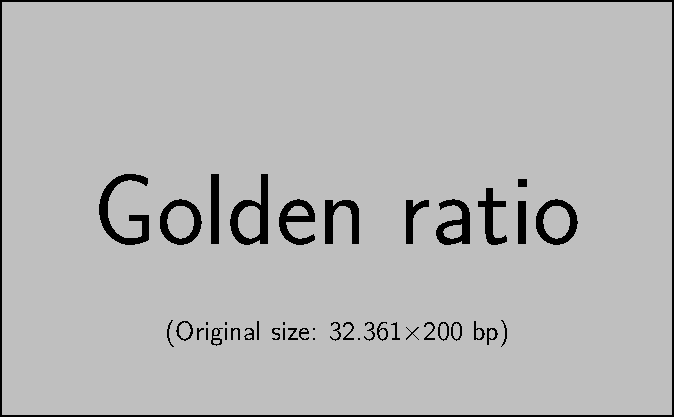
\includegraphics{placeholder_images/example-image-golden.pdf}
    \caption[Charge-transer and basic working mechanism of a Li-ion cell]{Simplified representation of charge-transfer
    process and illustration of basic working mechanism of a Li-ion cell.}
    \label{fig:chargetransferprocess}
\end{figure}

At fully  charged condition,  the majority  of Lithium in  the system  is stored
within  the  negative  electrode  microstructure.  During  discharge,  \ch{Li^0}
atoms  diffuse  out of  deep  interstitial  sites  towards  the surface  of  the
particles  in  the negative  electrode.  At  the surface  (electrode-electrolyte
interface),  a charge-transfer  process takes  place according  to Butler-Volmer
kinetics~\cref{eq:butlervolmer}, leading to the  formation of \ch{Li^+} ions and
electrons.  The electrons  are passed  to the  external circuit  through \ch{Cu}
current collectors  onto which  the conductive matrix  composed of  the negative
electrode material and binders is coated.  The \ch{Li^+} ions travel through the
electrolyte phase,  crossing the  separator membrane  to the  positive electrode
where they  encounter an  electron influx  from the  external circuit.  A charge
transfer  reaction  takes  place  at  the  surface  of  the  positive  electrode
particles, leading to the formation of neutral \ch{Li^0} atoms that diffuse into
the positive electrode microstructure.

During  the   charging  process,  the   reverse  phenomena  occur.   Lithium  is
de-intercalated  from  the  positive  electrode and  a  similar  charge-transfer
happens  at the  surface,  leading  to the  formation  of  \ch{Li^+} ions  which
reach  the  negative  electrode  by   passing  through  the  separator.  At  the
surface  of  the  negative  electrode particles,  these  ions  absorb  electrons
from  the  external circuit,  leading  to  the  formation of  neutral  \ch{Li^0}
that   diffuses  into   interior   vacant  spaces   in   the  layered   graphite
electrode. The  charge-transfer mechanism  and sequence  of events  are depicted
in~\cref{fig:chargetransferprocess}.
\Cref{eq:NegElectrodeRxn,eq:PosElectrodeRxn} summarise the reactions during the
charging and discharging process at the surfaces of both electrode materials.
\begin{align}
    \ch{Li_{$x$} C                            &<=>[\tiny{discharge}][\tiny{charge}] C + $x$ Li^+ + $x$ e^-}\label{eq:NegElectrodeRxn}\\
    \ch{Li_{1-$x$} M O2 + $x$ Li^+  + $x$ e^- &<=>[\tiny{discharge}][\tiny{charge}] LiMO2}\label{eq:PosElectrodeRxn}
\end{align}
where    \ch{M}   represents    a    transition   metal    compound   such    as
\ch{Ni_{1/3}Co_{1/3}Mn_{1/3}}   (NMC),   \ch{Ni_{0.8}Co_{0.15}Al_{0.05}}   (NCA)
amongst other  choices~\cite{Reddy2011}. Assuming  no loss of  cycleable Lithium
due to  parasitic side  reactions or  through other  mechanisms, the  process is
fully reversible.


The electrochemical potential at each electrode  is dependent upon the extent of
its  lithiation. An  empirical  relationship of  each  electrode's potential  as
a  function  of  its  stoichiometry  can be  obtained,  and  is  dependent  upon
the  specific design  and  material  properties of  each  active material  under
consideration. Finally, the \gls{ocv} of the cell is obtained by subtracting the
negative electrode potential from its positive electrode counterpart.


\section{Battery Modelling}

Through accurate model representations  of the electrochemical-thermal behaviour
of  the cell,  advanced monitoring  and control  strategies can  be deployed  to
tackle  the current  research  topics  in Li-ion  batteries  such as  increasing
cycle-life, improving operational  safety and performance~\cite{Plett2015}. Over
the past  two decades, efforts  have been made  to construct accurate  models to
describe  the physical,  electrical, thermal,  electrochemical and  system-level
performance  of  Li-ion  cells,  leading  to  modelling  strategies  of  various
level  of  sophistication.  For  the  interested  reader,  large  in-roads  into
understanding  the breadth  and  depth  of modelling  of  lithium ion  batteries
can  be  made   from  perusing  comprehensive  books  on  this   topic  such  as
those  by Plett~\cite{Plett2015},  Hariharan~\cite{Hariharan2017}, and  Rahn and
Wang~\cite{Rahn2013}.

The  need  to  address  the  operational challenges  of  lithium  ion  batteries
in   an   embedded   environment   such  as   on-board   an   electric   vehicle
has   led   to  an   increased   impetus   on   the  development   of   advanced
\glspl{bms}~\cite{Bergveld2002}. In vehicular  applications, the only measurable
quantities  of  a  lithium  ion  cell are  its  terminal  voltage,  current  and
temperature. This implies  that several internal states of the  cell such as its
\gls{soc}, whose  real-time computation is  vital to the optimal  performance of
the cell, need to be estimated from these available measurements. Therefore, the
performance  of  a \gls{bms}  for  tasks  such  as  online state  estimation  is
dependent upon  the fidelity  of the underlying  cell model  used. Sophisticated
models of the  cell enable these quantities to be  estimated more accurately and
facilitate the implementation  of advanced control algorithms.  Therefore, it is
imperative  that  the cell  model  used  is suitable  for  being  embedded in  a
real-time \gls{bms}.

Most battery  models have the primary  goal of accurately predicting  the cell's
terminal  voltage  at each  time-step.  This  is so  that  the  output from  the
predictor routine  can be compared  to the  measured voltage and  the difference
between them  may be used in  a suitable corrector-subroutine to  improve future
prediction.  The combined  information from  the model  and measurement  is then
blended in a suitable way to estimate the cell's \gls{soc}.

More   advanced  models   strive   to  provide   insight   into  various   other
physico-chemical quantities  that could  affect the health  of the  battery. The
field of  Li-ion battery modelling can  be classified into two  broad categories
---
\begin{enumerate*}[label=\roman*)]
    \item empirical/ad-hoc \glspl{ecm}, and
    \item detailed  \glspl{pbm} that are based  upon first principles.
\end{enumerate*}
However, these  two approaches are typically  at loggerheads with each  other in
the aspect of their computational complexity.

\subsection{\glsfmtlong{ecm}s}

\glspl{ecm}  employ circuit  elements  such as  voltage  sources, resistors  and
capacitors to  model the behaviour  of batteries at their  electrical terminals.
The cell's  thermal subsystem may  also be  modelled by an  analogous electrical
circuit. The  parameters of the  circuit are  typically functions of  the cell's
current, \gls{soc} and  temperature and can be implemented as  a lookup table by
curve-fitting  the model  to experimental  data. Using  such equivalent  circuit
models, two simple methods are available to compute the cell's \gls{soc} ---
\begin{enumerate*}[label=\itshape\alph*\upshape)]
    \item manufacturer-supplied  lookup table or graph of \gls{ocv} versus \gls{soc}, and
    \item numerically integrating the charge passed in and out of the cell over time, commonly referred to as coulomb counting.
\end{enumerate*}
Both methods are computationally  amenable for small-scale embedded applications
like  consumer  electronics;  however,  neither  one is  robust  to  handle  the
stringent demands in performance imposed  by modern vehicular applications.

Advanced state estimation algorithms such  as nonlinear Kalman filters may still
be able to use \glspl{ecm} as the plant model and obtain reasonable estimates of
the  cell's  \gls{soc}~\cite{Plett2006,  Sun2011}. However,  the  usefulness  of
\glspl{ecm} is limited by the fact that their parameters are derived essentially
by a  curve-fitting process using a  standard set of training  data. Since these
models are  not based on  any physical phenomena,  their ability to  predict the
cell's general behaviour  is extremely poor especially when  subjects to current
profiles well  outside their training  realm. Another important  disadvantage of
equivalent circuit  models is that they  do not allow insights  into the various
internal states of the cell.

\glspl{ecm}  of  lithium  ion  batteries   have  been  extensively  studied  and
are  widely  applied.  However,  the aforementioned  difficulties  render  their
reliability and  accuracy questionable,  especially under highly  demanding load
profiles  experienced by  the battery  packs in  \glspl{xeV}. The  boundaries of
their  performance have  been well-quantified  (see~\cite{Plett2015,Plett2016}).
Although  various estimation  and control  algorithms continue  to be  developed
around them, the  \glspl{ecm} themselves are no longer the  subject of extensive
research. Hence, this thesis does not discuss them further.

\subsection{\glsfmtlong{pbm}s}

\glsreset{pbm}

\glspl{pbm} consist of  governing equations that construct a  realization of the
behaviour of the cell based  upon electrochemical principles such as equilibrium
thermodynamics,  material  diffusion  and  reaction  kinetics.  The  fundamental
advantage  to this  modelling approach  is that  it is  possible to  compute the
evolution of  internal states of  the cell  for arbitrary current  profiles. The
difficulty with  the physics-based  modelling approach  lies with  obtaining the
values  of all  the physical,  geometric, electrochemical,  thermal and  kinetic
parameters  of the  cell. Usually,  these parameters  are closely  guarded trade
secrets by cell cell manufacturers.

In  some  cases, it  may  be  possible to  obtain  a  subset of  these  physical
parameters  can be  obtained  by dissection  of cells  in  an inert  environment
followed  by further  characterisation  through specialised  lab equipment.  For
instance, Ecker~\etal~\cite{Ecker2015} demonstrate  the reverse-engineering of a
\SI{7.5}{\amphour} pouch cell by Kokam  Ltd.\ to obtain its physical parameters.
Nevertheless, this is a tedious process and is feasible only with access to such
specialised lab  equipment. Furthermore, the  results from these  experiments is
susceptible to characterisation errors as well as cell-to-cell variations due to
production spread. Therefore, some form of system identification method needs to
be employed  for estimating the rest  of the physical parameters  required for a
\gls{pbm}.  Furthermore, it  is  a common  practice to  rely  on published  data
for  the values  of  certain cell  parameters  that do  not  depend on  physical
construction, especially for those that remain universally true for a particular
li-ion chemistry.

The challenges involved  in model parametrisation is a research  exercise of its
own merit and  is not addressed in  this thesis. A redeeming factor  is that the
task of  parametrisation is a  one-off problem that  appears early in  the model
deployment  stage,  after which  the  rewards  of  superior performance  of  the
\glspl{pbm} can be reaped. Once  the model parameters are available, \glspl{pbm}
can be used in  aiding a deeper understanding of the working of  the cell and in
answering research  questions that could  otherwise not be answered  with simple
\glspl{ecm}. One area  of focus of this  thesis is to broach  a less-probed area
--- exploring  the possibility  of using  a \gls{pbm}  for the  \emph{design} of
pouch cells used in automotive applications. The author's findings on this topic
shall be presented in~\cref{ch:modelbaseddesign}.

A major disadvantage of \glspl{pbm} from an implementation point of view is that
solving for  the model's field  variables is time-consuming. In  particular, the
more  sophisticated  \glspl{pbm}  require  the use  of  multi-physics  \gls{pde}
solvers  and  hence  are  not  typically  suitable  for  embedded  applications.
Nevertheless,  for   high  performance   applications  such  as   in  automotive
\glspl{bms}  wherein   state-of-health  monitoring  is  crucial,   there  is  an
overwhelming  demand for  obtaining insight  into internal  cell variables.  For
instance, the real-time computation of surface concentration of \ch{Li^0} in the
solid particles enable  the \gls{bms} to avoid regulate power  flow into and out
of the cell to proactively avoid plating and degradation of the cell.

In view of this consideration, model  order reduction techniques are seen as key
enablers that facilitate in porting the  predictive powers of \glspl{pbm} into a
real-time microprocessor. This thesis shall therefore have a strong focus on



Doyle,  Fuller,  and  Newman~\cite{Doyle1993}  developed  an  isothermal  porous
electrode model of the cell capable of describing its internal variables such as
\begin{enumerate*}[label=\itshape\alph*\upshape)]
    \item potential on the solid particles,
    \item potential in the electrolyte solution,
    \item concentration of \ch{Li^0} in the solid particles,
    \item ionic concentration in the electrolyte solution, and
    \item molar flux density of lithium at the solid-electrolyte boundary.
\end{enumerate*}
The most popular computational implementation  of the \gls{dfn} equations is the
\gls{p2d} model.  In the  \gls{p2d} implementation, all  field variables  of the
\gls{dfn} model are  computed at each spatial location location  along the axial
thickness of the cell. The solid  concentration is computed within each particle
in a radial co-ordinate system that is  normal to the axial direction. The axial
and radial dimensions  are coupled at each particle's surface  through the molar
flux density describing the rate of  pore-wall flux that crosses from solid into
electrolyte or vice-versa. The \gls{p2d} implementation of the equations of the
\gls{dfn} model is shown in~\cref{tbl:dfneqns}.

Ragone plot

Different type of cells - Prismatic,  pouch and cylindrical. How pouch cells are
used in automotive industry acknowledge Tesla, but cite counter citations. Layer
photos etc

This  thesis  strives to  represent  all  physical  quantities in  the  standard
International  System  of Units  (SI-Units).  However,  there are  some  notable
exceptions \eg{} for the capacity of a  Li-ion cell, which is represented in the
practical units  of Ampere  hours (\SI{}Ah),  rather than the  base SI  Units of
Coulombs (\SI{}{\coulomb}).  Such exceptions  are made  taking into  account the
prevalent conventions in standard literature.

\fxnote{make a note in the introduction  chapter that the terms cell and battery
    are  used  interchangeably deviating  from  their  precise meaning,  \eg{}  cell
modelling and battery modelling}

% \cite{Grazioli2016a} goes crazy in reviewing the models out there.

% \cite{Seaman2014} provide a comprehensive survey  of the wide range of battery
% models out there.

Based on an isothermal description
Mention  that stuff  is  applicable for  both Lithium  ion  and Lithium  polymer
chemistries.


% -*- root: ../main.tex -*-
%!TEX root = ../main.tex
% this file is called up by main.tex
% content in this file will be fed into the main document
% vim:nospell textwidth=180 foldlevelstart=3 foldlevel=3

% \begin{table}[!htbp]
    \begin{table}[p]
        \centering
        \caption[]{}
        % \label{tbl:charSimspmp2d}
        \begin{threeparttable}
            \begingroup
            \makeatletter\def\f@size{10.0625}\check@mathfonts
            % \addtolength{\jot}{0.75em}
            \addtolength{\jot}{0.875em}
            \begin{tabular*}{\textwidth}{@{} l c r l r @{}}
                \toprule
                Region & Governing equations & \multicolumn{3}{c}{Boundary conditions} \\
                \midrule
                \multicolumn{1}{l |}{\rotatebox[origin=c]{+90}{\makecell{\small Electrodes \\ \small \linnegpos}}} &
                $\begin{aligned} % placement: default is "center", options are "top" and "bottom"
                    \vphantom{\diffp{c_\slsub}{r}{\mathrlap{r = R_\pl}}}
                    \diffp{c_\slsub}{t} &= \frac{D_\slsub}{r^2}\diffp{}{r}\left(r^2 \diffp{c_\slsub}{r} \right) \\
                    \vphantom{\diffp{c_\text{e}}{x}{\mathrlap{x = l_\text{tot}}}}
                    \varepsilon_l \diffp{c_\text{e}}{t} &= \diffp{}{x}\left(D_\effl
                    \diffp{c_\text{e}}{x} \right) + (1 - t^0_\text{+}) a_\slsub j_l \\
                    \vphantom{\diffp{\phi_\text{e}}{x}{\mathrlap{x = 0}}} 0 &= \diffp{}{x}\left(\kappa_\effl \diffp{\phi_\text{e}}{x}\right) + \diffp{}{x}\left(\kappa_\effl \frac{2 R T(t)}{F} (t^0_{+}-1)\diffp{ \ln c_\text{e}}{x}\right) \\
                    \vphantom{\sigma_\effl\!\diffp{\phi_\slsub}{x}{\mathrlap{\substack{\vphantom{\displaystyle M}x = x_\text{pos/sep}\\x = x_\text{neg/sep}}}}} a_\slsub F j_l &= \diffp{}{x}\left(\sigma_\effl \diffp{\phi_\slsub}{x}\right) \\
                    % j_l &= k_\lr c^\alpha_\text{e}\left(c_\slmax - c_\slsurf\right)^\alpha c^\alpha_\slsurf\left( \exp\left(\frac{\left(1-\alpha\right)F}{R T}\eta\right) - \exp\left(-\frac{\alpha F}{R T}\eta\right) \right)
                    j_l &= 2 k_\lr \sqrt{c_\text{e}\left(c_\slmax - c_\slsurf\right) c_\slsurf} \sinh \left(\frac{0.5 F}{R T(t)} \eta_l \right)
                \end{aligned}$ &
                $\begin{aligned}
                    \vphantom{\diffp{c_\slsub}{r}{\mathrlap{r = R_\pl}}} \diffp{c_\slsub}{r}{\mathrlap{r = 0}}\hspace{1mm} &= 0, \\
                    \vphantom{\diffp{c_\text{e}}{x}{\mathrlap{x = l_\text{tot}}}} \diffp{c_\text{e}}{x}{\mathrlap{x = 0}}\hspace{1mm} &= 0, \\
                    \diffp{\phi_\text{e}}{x}{\mathrlap{x = 0}}\hspace{1mm} &= 0, \\
                    \sigma_\effl\!\diffp{\phi_\slsub}{x}{\mathrlap{\substack{\vphantom{\displaystyle M}x = x_\text{pos/sep}\\x = x_\text{neg/sep}}}}\hspace{1mm} &= 0, \\
                    % {}&\textemdash{}{}
                    {}&\xdash[1.25em]{}
                \end{aligned}$ &
                $\begin{aligned}
                    \diffp{c_\slsub}{r}{\mathrlap{r = R_\pl}}\hspace{1mm} &= \frac{-j_l}{D_\slsub} \\
                    \diffp{c_\text{e}}{x}{\mathrlap{x = l_\text{tot}}}\hspace{1mm} &= 0 \\
                \vphantom{\diffp{\phi_\text{e}}{x}{\mathrlap{x = 0}}} \phi_\text{e}\Bigr\rvert_{\mathrlap{x=l_\text{tot}}} \hspace{1mm}&= 0 \\
                % \sigma_\effl\!\diffp{\phi_\slsub}{x}{\mathrlap{\subalign{x&=0\\x&=x_\text{tot}}}} &= \frac{-I}{A} \\
                \vphantom{\sigma_\effl\!\diffp{\phi_\slsub}{x}{\mathrlap{\substack{\vphantom{\displaystyle M}x = x_\text{pos/sep}\\x = x_\text{neg/sep}}}}} \sigma_\effl\!\diffp{\phi_\slsub}{x}{\mathrlap{\substack{\!\!\!\!\!x=0\\x=x_\text{tot}}}}\hspace{1mm} &= \frac{-I}{A} \\
                % \sigma_\effl\!\diffp{\phi_\slsub}{x}{\mathrlap{\substack{\begin{mysubarray} x &=0 \\ x &=x_\text{tot}\end{mysubarray}}}} &= \frac{-I}{A} \\
                % {}&\textemdash{}{}
                {}&\xdash[1.25em]{}
            \end{aligned}$ &
            $\begin{aligned}
                \vphantom{\diffp{c_\slsub}{r}{\mathrlap{r = R_\pl}}}\refstepcounter{equation}(\theequation)\label{eq:dfnsoliddiff} \\
                \vphantom{\diffp{c_\text{e}}{x}{\mathrlap{x = l_\text{tot}}}} \refstepcounter{equation}(\theequation)\label{eq:dfnliquiddiff} \\
                \vphantom{\diffp{\phi_\text{e}}{x}{\mathrlap{x = 0}}} \refstepcounter{equation}(\theequation) \\
                \vphantom{\sigma_\effl\!\diffp{\phi_\slsub}{x}{\mathrlap{\substack{\vphantom{\displaystyle M}x = x_\text{pos/sep}\\x = x_\text{neg/sep}}}}} \refstepcounter{equation}(\theequation) \\
                \vphantom{\left(\frac{0.5 F}{R T(t)} \eta \right)} \refstepcounter{equation}(\theequation)
            \end{aligned}$ \\
            \bottomrule
        \end{tabular*}
        \endgroup
        \begin{minipage}{\textwidth}
            \bigskip
            \begin{flushleft}
                \raggedright
                \makeatletter\def\f@size{14}\check@mathfonts
                $\begin{alignedat}{2}
                    & \text{\textbullet{} } c_\text{e} &  & \coloneqq c_\text{e}(x,t), \quad  \{x \in [0,l_\text{tot}],\, (x=0)\symbol{"2259} \text{\footnotesize pos/Alcc},\, (x=l_\text{tot})\symbol{"2259} \text{\footnotesize neg/Cucc}\}  \tnote{\dagger}                                                                                                                                                                  \\
                    & \text{\textbullet{} } \phi_\text{e} &  & \coloneqq \phi_\text{e}(x,t)\\
                \end{alignedat}$
                \\[0.5em]
                \fbox{\raggedright \small  \linnegpos}
                $\begin{alignedat}{2}
                    % & \mathbf{\textbf \linnegpos} & {} \\
                    & \text{\textbullet{} } c_\slsub   &  & \coloneqq c_\slsub(r,t), \quad  \{r \in [0,R_\pl],\, (r=0)\symbol{"2259} \text{\footnotesize  particle center},\, (r=R_\pl)\symbol{"2259} \text{\footnotesize particle surface}\}              \\
                    & \text{\textbullet{} } c_\slsurf &  & \coloneqq c_\slsub(r=R_\pl,t)\\
                    & \text{\textbullet{} } \phi_\slsub &  & \coloneqq \phi_\slsub(x,t)\\
                    & \text{\textbullet{} } j_l          &  & \coloneqq j_l(x,t) \\
                    & \text{\textbullet{} } \sigma_\effl &  & = \sigma_l \cdot \varepsilon_l \\
                    & \text{\textbullet{} } \eta_l        &  & \coloneqq \eta_l(x,t) = \phi_\slsub(x,t) - \phi_\text{e}(x,t) - \mathcal{U}_l(c_\slsurf) \\[0.5em]
                \end{alignedat}$
                % \medskip
                \fbox{\raggedright \small  \linnegseppos}\\[0.5ex]
                $\begin{alignedat}{2}
                    & \text{\textbullet{} } D_\effl    &  & = D \cdot \varepsilon_l^{\text{brugg}_l}                                                                                                                                                  \\
                    & \text{\textbullet{} } \kappa_\effl &  & = \kappa \cdot \varepsilon_l^{\text{brugg}_l} \\
                    & \text{\textbullet{} } D        &  & \coloneqq D(c_\text{e},T) = 10^{-4} \times 10^{-4.43 - \frac{54}{T(t) - 229 - 5\times10^{-3} c_\text{e}(x,t)} - 0.22\times10^{-3} c_\text{e}(x,t)}               \\
                \end{alignedat}$
                \\
                \makeatletter\def\f@size{14}\check@mathfonts
                $\begin{alignedat}{2}
                    & \text{\textbullet{} }  \kappa   \: \quad&  & \coloneqq \kappa(c_\text{e},T)\, = \parbox[t]{11.60cm}{\raggedright $\scriptstyle 10^{-4} \times c_\text{e}(x,t)\Big(-10.5 + 0.668\times10^{-3} c_\text{e}(x,t) + 0.494\times10^{-6} c_\text{e}^2(x,t) + \big(0.074 - 1.78\times10^{-5}c_\text{e}(x,t) - 8.86\times10^{-10}c_\text{e}^2(x,t)\big)T(t) + \big(-6.96\times10^{-5} + 2.8\times10^{-8} c_\text{e}(x,t)\big)T^2(t)\Big)^2$}\\
                \end{alignedat}$
            \end{flushleft}
        \end{minipage}
        \bigskip
        \footnoterule{}
        \begin{tablenotes}
        \item[\dagger] \footnotesize{This definition of the global axial domain $x$, spanning the cell thickness applies for all variables dependent on axial spatial position. Hence the domain definition for $x$ is not repeated elsewhere for the sake of brevity.}
        \end{tablenotes}
    \end{threeparttable}
\end{table}


% write about lumped thermal model equations here. Point out to relevant
% parameters


% \fxnote{Where does  this paragraph go? End  of this section/end of  chapter or
% even  last  chapter?}  The  identification of  individual  parameters  of  the
% \gls{dfn} model  remains a  key area  in battery  modelling that  remains only
% partially  explored. Nevertheless,  this effort  is critical  to ensure  rapid
% adoption  of any  physics-based  model and  sophisticated control  algorithms.
% The  state of  the  art in  this  area, the  challenges  involved and  current
% efforts  in  this  direction are  explored  in~\cref{ch:futurework}.  Although
% sensitivity  analysis  of  the  \gls{dfn} parameters  has  been  performed  in
% literature, \fxnote{citation here} the extent to which parameter uncertainties
% influence  the   numerical  values  in  the   $A,  B,  C$  and   $D$  matrices
% of~\Cref{eq:LTIstatespace} has not yet been attempted. In continuation of this
% research aspect, the order of magnitude  shift in eigen/singular values of the
% relevant system matrix also need to be quantified to enable an informed choice
% about stability of such models for real-time implementations.


\setcounter{chapter}{3}
% % -*- root: ../main.tex -*-
%!TEX root = ../main.tex
% this file is called up by main.tex
% content in this file will be fed into the main document
% vim:textwidth=80 fo=cqt

%level followed %by section, subsection


% ----------------------- paths to graphics ------------------------

% change according to folder and file names
\graphicspath{{4/figures/}}
% ----------------------- contents from here ------------------------

\todo{uncomment and edit the intro in the source code later on}

% Battery modellers face the classic  conundrum of conjuring physics-based battery
% models that remain  amenable for control applications.  Firstly, the contrasting
% nature of this modelling objective is presented. Secondly, prior attempts by the
% research community to  tackle this issue is briefly examined.  A suitable family
% of models  from the broad  category of reduced-order  models is identified  as a
% promising  candidate  for implementation  in  controls  applications. Next,  the
% drawbacks of this family of models is  discussed in detail. The state of the art
% implementation for tackling these drawbacks  is presented and their inadequacies
% are discussed.


\todo{Write the chapter. Finally come back to summarize this}


% The following efforts/trials were done (failures)
% \begin{itemize}
%     \item first attempt
%     \item second attempt
% \end{itemize}
% The following successes were achieved.
% \begin{itemize}
%     \item first attempt
%     \item second attempt
% \end{itemize}


% At the  end of this  chapter, we have a  control oriented reduced  order battery
% model amenable for use in real-time applications for SOC, SOH etc.\ estimations.


Control-Oriented  models can  be considered  synonymous with  the term  `Reduced
Order Models'. This is because the complexity of physics-based models inherently
necessitates the  use of a low  order model. In  this thesis, the two  terms are
used interchangeably.


\section{Reduced Order Models: A New Classification Scheme}\label{sec:classificationscheme}

Jokar~\etal~\cite{Jokar2016}  provide  a  comprehensive review  of  the  various
categories  of  reduced  order  physics  based  battery  models.  However,  this
work  does  not aim  to  classify  models  based on  time-vs-frequency  domains.
Fan~\etal{}~\cite{Fan2015}  conducted  a  review   of  reduced  order  modelling
methods, but  only provide an  overview of  deriving and implementing  models in
these  dual domains  without expository  analysis  of the  implications of  this
modelling choice. Unlike~\cite{Jokar2016}, this review  did not aim to provide a
classification  of various  reduced order  models, but  instead emphasises  on a
broad survey of relevant methodologies  and tools towards obtaining such models.
Hence,  neither~\cite{Jokar2016}  nor~\cite{Fan2015}  provide insight  into  the
rubrics and  implications of  the choice  of modelling in  either of  these dual
domains. Although in principle, the transformation between them follows standard
mathematical  practices,\todo{citation(s)  needed?}availability  of  models  for
final implementation  in the time domain  aids immediate uptake by  industry for
adoption  in online  \gls{bms}s. Treatment  of  reduced order  models from  this
aspect  is so  germane to  the central  hypothesis of  this chapter,\todo{can  a
simple time  domain model  do the  job?} that  the author  of this  thesis feels
compelled to undertake  a simpler classification exercise within  the context of
suitability for online implementation.


In this discussion,  various modelling methodologies and  their resultant models
are viewed  as a single  continuum and  consequently this thesis  discusses them
from such a unified perspective. Furthermore,  there is also a need to highlight
the  salient  works among  the  more  recent  advances  and extensions  to  then
prevailing  models published  since~\cite{Jokar2016} and~\cite{Fan2015}.  Hence,
the specialised  review of  reduced order modelling  literature covered  in this
section intends to supplement --- not  supplant --- the breadth of modelling art
covered between them. In particular, care  has been taken to minimize repetition
of  background art  already analysed  in these  aforementioned review  articles,
thereby striving  to report the  subset of prior  research that is  pertinent to
illustrate the  new classification scheme  introduced here. The author  does not
aim to adhere  to a chronological presentation of such  background art. Instead,
the salient  model families are  introduced in  the context of  discussing their
significance within a particular modelling technique.



Physics-based control-oriented models  can be classified as belonging  to one of
the following categories.\todo{just enumerate my classification in-line here} It
is important to distinguish between models that are derived directly in the time
domain versus  those that are  derived first in  the frequency domain  and later
converted to time domain.
\todo{enumerate all the desirable characteristics and criterion upon which
models are to be evaluated}


In  principle,  any modelling  method  that  yields a  time domain  mathematical
description of physical  phenomena that is lower in  computational complexity by
an arbitrary magnitude  than the original \gls{dfn} model can  be considered for
further investigation. In the absence of a canonical, quantitative definition of
what  constitutes a  reduced  order model,  the number  of  candidate family  of
models  to  consider  is  overwhelmingly large\todo{is  it  appropriate  to  use
such  language?}.  In  practice,  the  constraints  and  challenges  imposed  by
the  scope  of  this  work, \viz{}  suitability  for  real-time  implementation,
limits  the  choice  of  candidate  modelling  families.  For  instance,  models
relying  primarily on  classical finite  difference~\cite{Smith2006}, Galerkin's
approximation~\cite{Dao2012} or Galerkin's projection~\cite{Fan2018} methods for
transformation  and order  reduction  of  one or  more  field  variables of  the
\gls{dfn} model  are excluded. This is  done in view of  the impracticability of
implementing  such  models in  a  resource-constrained  environment such  as  an
embedded \gls{bms} controller.


Owing to  the low entry-barrier for  adoption in a real-time  controller logging
data samples  at specific time intervals,  this chapter focusses on  models that
are cast  in a  form for final  implementation in the  time domain.  This choice
implies the exclusion of those models  that are derived and implemented entirely
in the frequency domain. For the  sake of readers interested in frequency domain
methods, the discussion here briefly introduces salient literature employing the
Padé  approximation method  that serves  as  a backbone  of a  wide variety  of
frequency domain models.


\todo{can  mention  that  most  frequency domain  models  are  impedance  models
suitable for offline simulation eg An electrochemistry-based impedance model for
lithium-ion batteries}


The     transfer     function     oriented    Padé     approximation     method
for    low    order    physics-based     battery    modelling    pioneered    by
Forman~\etal{}~\cite{Forman2011a}    has   gained    widespread   adoption    in
the    areas     of    cell     design~\cite{Marcicki2013},    charge-trajectory
optimisation~\cite{Bashash2010},    controller    design~\cite{Perez2015}    and
state    estimation~\cite{Marcicki2013,Moura2012}.     Although    Prasad    and
Rahn~\cite{Prasad2013} present  an online identification  of a subset  of ageing
parameters using a Padé model and a recursive least squares algorithm, specific
implementation details such as the transformation of the Padé reduced impedance
to  discrete-time  difference  equations  was not  provided.  Padé  models  are
typically limited  to offline  applications owing  to the  aggressive trade-offs
required in the approximation order to maintain accuracy. Those models truncated
to  very low  Padé  order exhibit  poor  fidelity and  perform  no better  than
classical  equivalent circuit  models,  although recent  research attempts  have
focussed  to  mitigate  this  drawback~\cite{Yuan2017a,Yuan2017}.\todo{Should  I
discuss how they mitigated this?}


Smith~\etal{}~\cite{Smith2007}  pioneered   a  semi-hybrid   modelling  approach
to  reduced  order  modelling  and  obtained closed  form  expressions  for  all
electrochemical field variables  in the frequency domain  except for electrolyte
concentration and  potential (which were  solved separately using  the classical
finite difference discretization method). To the author's knowledge, this is the
earliest  published  instance  wherein  all  the  dynamics  of  the  full  order
model were  completely retained  in the frequency  domain. This  was facilitated
through  the use  of  transcendental  transfer functions  that  helped to  avoid
the  accuracy  degradation  brought  about  by  truncation  techniques  such  as
Padé  approximation. A  composite impedance  model was  obtained that  was then
converted  to  a  \engordnumber{12}  order state  space  model  through  residue
grouping  and truncation  techniques.  To  the knowledge  of  this author,  this
represents the first  instance in published literature  demonstrating a complete
hybrid  modelling workflow.  This model  was  capable of  predicting the  cell's
terminal voltage  within \SI{1}{\percent} of  a full-order \gls{dfn}  model. The
lumped impedance  model was  derived for  the frequency  range of  interest from
\SIrange{0}{10}{\hertz}.

This modelling effort  by Smith~\etal{} was the  first of its kind  to provide a
physics-based  battery model  for  implementation in  the classical  state-space
formulation
\begin{equation}\label{eq:statespace}
    \begin{aligned}
        \dot{x} &= Ax + Bu \\
        y &= Cx + Du
    \end{aligned}
\end{equation}
that is amenable for controller  design and  further system-level simulation
studies \eg{}  as a component in a (hybrid) electric vehicle drivetrain.


The requirement of a relatively large number of state variables (12) to describe
the system dynamics dilutes the effectiveness of state estimation algorithms. In
the classical isothermal implementation of  this model, with the cell's terminal
voltage being the only measured quantity, the observablity of the model degrades
significantly. Although Smith~\etal{} performed  an observablity analysis of the
model in  a noise-free context,  the presence  of process noise  (via unmodelled
electrochemical phenomena  and parameter uncertainties) coupled  with corruption
of measurement  values through  sensor noise in  a harsh  electrical environment
such as  in an  vehicle's drivetrain,  makes this  model unattractive  for state
estimation tasks in an online embedded application.


Several attempts have been undertaken to  improve and extend the ideas pioneered
in  Smith~\etal{}~\cite{Smith2007}.  Lee~\etal{}~addressed  a  critical  missing
aspect  of~\cite{Smith2007}, \viz{}  the derivation  of transcendental  transfer
functions  for  both the  electrolyte  concentration  and its  potential.  These
transfer  functions  were  obtained  by  using  a  Sturm-Liouville  approach  by
retaining  the first  five modes  of  the eigenfunction  expansion, as  detailed
in~\cite{Lee2012}. To the  author's best knowledge, this is  the first published
work wherein  all electrochemical  field variables of  the \gls{dfn}  model were
considered  for inclusion  in a  deterministic model  order reduction  procedure
whilst retaining the derivation entirely in the frequency domain.


Obtaining  closed form  expressions for  the electrolyte  variables achieved  in
Lee~\etal{} also has an important computational implication. With these capstone
derivations serving to completing the model description in the frequency domain,
all  electrochemical  variables of  the  \gls{dfn}  model  could now  be  solved
independently at any  desired spatial location, \eg{} at  the current collectors
and separator  interfaces. Until  this point,  the state of  the art  in reduced
order  modelling invariably  necessitated  the solution  of all  electrochemical
quantities at  multiple node locations along  the thickness of each  cell layer,
adding  to the  computational burden.  This is  a significant  deterrent to  the
adoption  of such  models if  the intended  purpose of  the model  is to  simply
predict the cell's terminal voltage.


Furthermore,  Lee~\etal{}~\cite{Lee2012a} also  devised the  \gls{dra}, a  novel
algorithm  to systematically  transform  all  transcendental transfer  functions
to  the  time domain   to  obtain  the  standard  state-space   model  given  by
\cref{eq:statespace}. The  author of  this thesis  considers the  formulation of
the  \gls{dra}  as a  breakthrough  contribution  that  has helped  in  bringing
physics-informed  time domain  models a  step  closer  to online  implementation
without   having  to   resort   to   forming  a   lumped   impedance  and   then
truncating  it  suitably.  Lee~\etal{}~\cite{Lee2014} then  extended  this  work
for  a  wider range  of  operation  across  various \gls{soc},  temperature  and
C-rates.  Although the  final  state space  model is  simple  to implement,  the
classical  \gls{dra} scheme  proposed  by Lee~\etal{}  suffers from  significant
computational bottlenecks  in forming the required  block-Hankel matrices during
the  model-derivation  phase.  A   memory-efficient  version  of  the  \gls{dra}
exploiting the  skew-symmetric structure of  these Hankel matrices  was proposed
in  Gopalakrishnan~\etal{}~\cite{Gopalakrishnan2017}  resulting  in  drastically
reduced requirements for physical memory and processing power.


In both the original  as well as the improved \gls{dra},  the computation of the
eigenfunction modal expansion of electrolyte concentration transfer function was
computationally intensive.  A less  severe disadvantage with  the transcendental
transfer  functions  associated  with  the electrolyte  concentration  was  that
their  derivation  entailed  mathematically  cumbersome  symbolic  manipulations
that  dictated  the   need  of  a  capable  \gls{cas}   package.  Although  from
a  stand-alone  viewpoint  this  requirement  does  not  seem  to  be  critical,
the  Ho-Kalman  algorithm   that  forms  a  core  component   of  the  \gls{dra}
schemes  is  steeped in  numerical  linear  algebra routines.  Furthermore,  for
facilitating  state  estimator  and  controller designs,  it  is  convenient  to
implement the resultant  state-space model in a  classical numerical computation
environment   such  as   \textsc{MATLAB}.  Taking   these  into   consideration,
Rodriguez~\etal{}~\cite{Rodriguez2017}  introduced a  simplified computation  of
the electrolyte  concentration transfer  function by  applying the  variation of
parameters  (VOP)  scheme.  With  this  final  improvement,  the  hybrid  scheme
envisaged originally by Lee~\etal{} can  be considered feature-complete with low
computational  requirements  during  both model  derivation  and  implementation
phase.


A  key  drawback  of  the  transcendental  transfer  function  approach  is  the
requirement for  linearisation at  a specific \gls{soc}.  This implies  that the
entries in  the matrices of the  state space model depends  on the linearisation
point.  In all  the  published  works employing  this  approach, these  transfer
functions were obtained  by linearising the \gls{p2d} equations  at an operating
point of  \SI{50}{\percent} \gls{soc}. The requirement  of linearisation renders
the  model usable  only  in  a narrow  range  of  \gls{soc}s. Furthermore,  this
adversely affects the usability of the model for state estimation tasks, wherein
the \gls{soc} is in fact an unknown quantity and is to be estimated.


In order  to extend  the model's  range of  validity, Lee~\etal{}~\cite{Lee2014}
proposed  a  simple model-blending  approach  by  interpolating between  several
linear models pre-computed at  different \gls{soc} and temperature combinations.
To guarantee robustness during cross-over, a  naive approach is to incorporate a
large  number  of  break-points  in  the  look-up  table.  Since  the  model  is
intended  for  online  operation,  this would  entail  significant  requirements
of  both operating  memory  and non-volatile  storage.  An alternative  approach
is  to  implement  a  fairly  coarse  break-point  table  with  a  sophisticated
changeover  mechanism. However,  this  demands careful  tuning  of the  blending
parameters  and  gain values,  an  in-depth  treatment  of  which has  not  been
detailed in Lee~\etal~\cite{Lee2014}.  Furthermore, employing these interpolated
matrices---whose  entries are  obtained  from pre-computed  matrices at  various
\gls{soc}s and temperature---for state-estimation  creates a subtle cyclic loop.
The stability  of this feedback loop  hence introduced has not  been analysed in
literature.  This  renders the  idea  of  state-estimation using  such  run-time
interpolated models  questionable.


The author  of this thesis hypothesises  that any perceivable drawbacks  such as
non-smooth changes  in \gls{soc} estimates  arising from using  blended matrices
could  be potentially  mitigated by  using  smoothing filters  and other  ad-hoc
apparatus.  However,  there  exists  no  published  work  that  discusses  these
engineering aspects. Coupled with the absence  of a theoretical analysis of loop
stability,  these  models  are  deemed  as  not  being  suitable  for  immediate
adoption  by  industry, at  least  until  these  aforementioned gaps  have  been
addressed  satisfactorily.  The non-linear  state  variable  model presented  by
Guo~\etal{}~\cite{Guo2017} aims to  address this issue by  formulating a reduced
order model in  the frequency domain by eliminating  linearisation. However, the
online solution of the model entails an complex prediction-refinement procedure,
loosely defined as implicit and explicit solution methods, for each subsystem of
the  \gls{dfn}  model.  The  formulation  of the  final  model  is  not  clearly
illustrated and  in the views of  this author, is not  easily comprehensible. In
the absence  of actual source  code, a numerical  example or pseudo-code  of the
model reduction workflow could have immensely helped with the reproducibility of
the results claimed in the work.


Physics-inspired                        equivalent                       circuit
models~\cite{Prasad2012,Prasad2014,Zhang2017,Cheng2017,Merla2018} are a class of
hybrid  models  that  have  rapidly  gained  prominence  since  the  publication
of~\cite{Jokar2016}  and~\cite{Fan2015}. The  derivation of  the relevant  model
equations  is  performed   in  the  frequency  domain.   This  frequency  domain
representation is  then converted to  a form  suitable for implementation  as an
equivalent circuit. Prasad and Rahn~\cite{Prasad2014} extended their Padé order
reduced  model first  presented  in~\cite{Prasad2013} to  convert the  impedance
model into standard  equivalent circuits. A key point to  be highlighted is that
these family of models do not necessarily strive to retain the classical Randles
structure~\cite{Randles1947}  for   their  equivalent   circuit  representation.
Instead,  the  values  of  the  electrical circuit  components  such  as  series
resistance and  equivalent capacitance  are obtained through  various mechanisms
such as \gls{eis} measurements under load.  The biggest advantage of such models
is that  they serve  as drop-in replacements  to traditional  equivalent circuit
models whilst still  retaining their origins in physical  principles rather than
on empirical curve-fitting.


\todo{can perhaps  talk about SPM converted  to equivalent circuit by  Prasad in
the IEEE conference paper}


\Cref{ch:chapter6}  briefly presents  the author's  latest work  and preliminary
results towards  obtaining a similar physics-informed  equivalent circuit model.
This  modelling  effort is  a  direct  application  of  the gains  in  computing
efficiency  through  the  application  of the  improved  \gls{dra}  reported  in
Gopalakrishnan~\etal{}~\cite{Gopalakrishnan2017},   the  detailed   coverage  of
which  is performed  in~\cref{ch:chapter3}.  This work  intends  to address  the
hitherto  unexplored  gap  in  impedance  modelling, \ie{}  the  absence  of  an
equivalent impedance  model that  accounts for  the impedance  contribution from
all  electrochemical quantities  in the  \gls{p2d} model.  This physics-informed
impedance  model can  be  extended  to fit  parameter  values  of components  in
an  equivalent circuit  model,  \eg{} by  using  a standard  Levenberg-Marquardt
non-linear least squares fitting algorithm~\cite{Levenberg1944, Marquardt1963}.


A common characteristic of  all hybrid models is the lack  of a physical meaning
to their  model parameters. This  severely limits  the insights offered  by such
models  into  electrochemical  phenomena  internal  to  the  cell.  The  biggest
attraction  of  using physics-based  models  is  the possibility  of  predicting
phenomena such as cell degradation, \eg{} through computation of the solid phase
surface concentration  and potentials  in a  vehicular application,  since their
exact  load profile  cannot be  simulated a-priori.  In this  scenario, a  model
capable of implying a direct and causal relationship between a group of physical
parameters and internal  overpotentials at various spatial  locations within the
cell serves  as a powerful  tool for  in-situ lifetime estimation  of batteries.
Although the  circuit components  of physics-informed equivalent  circuit models
and the  state-space models discussed here  trace their origins to  the original
parameters of  the \gls{dfn}  model, their  final numerical  values do  not bear
even a  semblance of this relationship.


With  goal   of  translating   physical  parameters  into   circuit  components,
Zhang~\etal{}~\cite{Zhang2017} presented a lumped equivalent circuit model based
on Padé  approximation and  model truncation. However,  the sensitivity  of the
final model  values owing to perturbation  in the original model  parameters was
not  evaluated.  Consequently, there  is  a  lack  of  clarity in  the  relative
importance  of physical  parameters  and their  influence  on circuit  component
values.


Merla~\etal{}~\cite{Merla2018} introduced  an equivalent circuit model  that can
be  parameterised by  attempting a  systematic  decoupling of  the kinetics  and
diffusion at  both electrodes  and the  electrolyte. Although  these interacting
phenomena can be complex to resolve  over all length and time-scales, acceptable
trade-offs in  accuracy was  demonstrated to be  achievable from  a system-level
simulation perspective. A  drawback of such models is that  key model parameters
such  as  solid  and  electrolyte   diffusion  coefficients  are  attributed  to
the  two electrodes  through  ad-hoc,  non-verifiable assumptions.  Furthermore,
in~\cite{Merla2018},  notable discrepancies  exist in  the values  of parameters
such as  electrolyte conductivity (obtained through  calculations from \gls{eis}
measurements) to  that typically reported  in literature. \todo{have  not talked
about SPM  inspired eq circuit model.  Is it necessary  to do so?. How  to frame
this. There are a few references that belongs to this kind}


It must be acknowledged that presently  there exists no modelling candidate that
provides  all desirable  characteristics  of  a reduced  order  model for  final
implementation in  the time domain. However,  it is strongly desirable  that the
majority  of the  final model  values  retain their  physical meaning,  yielding
system engineers and cell designers alike  with a direct and causal relationship
between  groups of  parameters and  their  influence on  the cell's  operational
performance. Since  this chapter seeks  to provide  a readily usable  model that
satisfies  all \todo{give  a number  here} criterion  for online  implementation
from,\todo{cite  figure} the  author  concludes that  at  present, the  benefits
offered by hybrid models do not decisively outweigh this drawback.


The working rubric of all time  domain reduced order models typically consist of
attempts to reformulate the original \gls{p2d}  model equations with the goal of
simplifying them.  In contrast to the  hybrid models, both the  model derivation
and  final  implementation  tasks  are  carried out  entirely  within  the  time
domain.  Whilst a  subset of  prior research  has focussed  only on  simplifying
certain aspects  of the  cell dynamics, \eg{}  solid diffusion,  other published
works  have aimed  at  providing a  simplified description  of  the time  domain
evolution of all  physical quantities of the cell. An  evaluation of the salient
literature  from both  these  approaches is  performed here.


In this discussion,  those models that entail computations with  medium or large
dense  matrices~\cite{Li2016,Xu2016,Corno2015}  or  involving concepts  such  as
fractional  order  derivatives~\cite{Sabatier2014,Sabatier2015, Li2017,  Mu2017,
Wang2017} shall not  be discussed. To this author, it  appears that the academic
community has  implicitly considered these models  to be so abstruse  that there
has not yet been a comparative  study pitting these models against the prevalent
art. Based  on published work,  it is not clear  on how such  models distinguish
themselves uniquely in the larger realm of reduced order battery.


A  few  \gls{pde}  simplification  techniques   in  the  time  domain,  such  as
Hilbert-Space  representation  and  singular   perturbation  were  presented  in
Manzie~\eta{}~\cite{Manzie2015}.  However, their  presentation lacks  expository
visual information  such as plots of  time domain evolution of the  internal and
terminal variables for dynamic load profiles. Furthermore, the authors failed to
provide a tabulated set of physical  parameters of the cell being simulated that
adversely affects the reproducibility of this  work. These methods have not seen
uptake  in academia  or  industry.  The author  of  this  thesis considers  this
presentation  to be  of a  cursory nature  and consequently,  they shall  not be
discussed here.


The  rest of  this section  discusses  several popular  families of  time domain
models. In  this section, a high-level  evaluation of their relative  merits and
weaknesses is  presented. The next section  presents a detailed analysis  of the
most promising  candidate among  these models with  the potential  to facilitate
faster adoption of physics based models in online applications. Further sections
discuss methodologies and  solutions that aim to address the  gaps identified in
this family of models. \todo{does this fit better at the end of this section}


In the \gls{dfn} model, the diffusion of Lithium in the solid phase is described
by the classical  Fick's second law~\cite{Fick1995}. In order to  solve for this
concentration  profile,  it  is  required to  discretise  every  spherical  node
(represented by the placement of a node in the axial direction) along its radial
direction (pseudo dimension). This dramatically  increases the overall number of
discretisation  nodes, adversely  impacting  the  computational efficiency.  The
impact of high node densities on  the computational requirements of the original
\gls{p2d}  model have  led researchers  to adopt  various mitigation  strategies
to  tackle  this  issue. In  contrast  to  the  pure  frequency domain  and  the
semi-hybrid/hybrid approaches discussed thus far, these attempts aim to provided
a simpler computational mesh, whilst retaining high fidelity. It should be noted
that high node  densities are mainly required near the  surface of the spherical
particles for the pseudo  \engordnumber{2} dimension. Similarly, such clustering
of nodes is desirable near the  separator and current collector interfaces along
the axial  dimension.\todo{need to define  `axial' at  the start of  the thesis}
Thus, a number  of model order reduction  strategies in the time  domain seek to
adopt  non-uniform node  spacing  towards lowering  the aforesaid  computational
issues\todo{citations needed}.


Computationally    efficient     pseudo-spectral    schemes     for    numerical
solution   of   \gls{pde}s   can be employed    by   choosing   discretisation
nodes    at    orthogonal    collocation     points    obtained    by    solving
for     the    zeros     of    certain     classes    of     polynomial    basis
functions~\cite{Ferguson1971,Trefethen2000,Boyd2001,Shizgal2015,Dutykh2016}.
Their accuracy extend beyond  the  algebraic  orders of that achievable with
classical  Finite  Difference,  Finite Element  or Finite Volume Schemes.
Northrop~\etal{}~\cite{Northrop2011} pioneered their application in battery
modelling by employing the Jacobi polynomials as underlying basis functions.
Suthar~\etal{}~\cite{Suthar2014} replaced the Jacobi polynomials with Chebyshev
polynomials to extend the applicability of the model to higher C-rates.
Bizeray~\etal{}~\cite{Bizeray2015}    provided   a detailed treatment of the
usage of Chebyshev discretisation  for   the  full   \gls{p2d} model   on  a
global  scale,  \ie{}  along  both   the  axial  and  radial directions.


The  reduced  number of  nodes  as  well as  their  clustered  placement at  the
desired  spatial  locations  enabled  by  these  discretisation  schemes  lowers
the   computational  burdens   of   simulating  a   physics-based  cell   model.
Gopalakrishnan~\etal{}~\cite{Gopalakrishnan2018} undertook a  hybrid approach by
retaining a  standard finite volume  discretisation in the axial  domain, whilst
adopting  the  Chebyshev  discretisation  only  for  the  critical  solid  phase
diffusion component in the radial direction. Albeit in time domain, the standard
\gls{p2d} equations, their boundary conditions and corresponding field variables
are  mathematically transformed  to the  Chebyshev space  within which  they are
solved.  The details  of this  transformation is  presented in  \cref{sec:hybrid
fv-spectral}  in  \cref{ch:chapter2}  for the  solid-phase  diffusion  equation.
Finally,  these solved  quantities  are  converted back  to  the physical  space
through  a corresponding  inverse transformation.  Although this  bi-directional
transformation is  algebraic in nature,  the requirement of running  a spatially
resolved model coupled with  such variable-transformation overheads render these
class  of  models unsuitable  for  online  implementation. The  contribution  of
Lee~\etal{}, \ie{} the  ability to solve for any electrochemical  variable at an
arbitrary  spatial  location by  completely  eliminating  the need  for  spatial
discretisation assumes particular significance in this context.


In all  non-uniform discretisation schemes  discussed here, the  implications of
using  a non-adaptive  support mesh  obtained by  the placement  of nodes  whose
locations are optimised a-priori, must be considered carefully. For instance, in
the long-term  usage of the cell  \eg{} in an electric  vehicle application, the
reaction front drifts  from separator back towards the  current collectors. This
is  due to  the exhaustion  of  Lithium at  the  surface of  particles near  the
separator  interfaces.  In  this  scenario,  the  solutions  produced  by  these
models could  be worse than  simpler models with uniform  mesh-density. Although
adaptive meshing strategies can be  employed for desktop simulation with minimal
effort,  it remains  to  be seen  if  this  can be  deployed  successfully in  a
resource-constrained environment  such as an embedded  \gls{bms} controller, and
hence warrants  further research.\todo{does  this fit  better in  the conclusion
chapter?}


The  computational  bottlenecks arising  due  to  discretisation in  the  radial
direction  have  motivated  researchers   to  explore  mesh-free  approaches  to
solve for  solid phase  concentrations. Subramanian~\etal~\cite{Subramanian2004}
pioneered  the concept  of employing  polynomial approximations  of the  Fickian
diffusion equation to solve for Lithium concentrations in the porous electrodes.
Here,  the solid-phase  surface  concentrations was  expressed  as a  correction
term  applied  to their  average  concentrations  which  was described  using  a
second degree polynomial. In  a follow-on study~\cite{Subramanian2005}, the same
authors  presented a  solution using  higher order  polynomials and  performed a
dimensionless analysis of their  proposed reformulation. In the \engordnumber{2}
and  \engordnumber{3}  order  solutions,  the polynomial  equation  for  surface
concentration was  accompanied by a  corresponding \gls{ode} for  describing the
temporal  evolution of  average concentration,  thereby leading  to a  system of
\gls{dae}s. Furthermore, Subramanian~\etal{}~\cite{Subramanian2007} demonstrated
the  application  of  polynomial  approximation  of  solid  phase  diffusion  by
simulating a complete \gls{dfn} model.


Using polynomial  approximation for the  solid phase concentration results  in a
drastic reduction  in the number  of \gls{dae}s needed  to solve the  full model
since now discretisation  needs to be performed only along  the axial direction.
The  polynomial  approximation  solution  applied   to  solve  for  the  surface
concentration in  the solid phase can  hence be viewed as  a dimension reduction
approach, as  it removes  the model's  dependence in  the radial  direction. The
textbook by  Carslaw and  Jaeger~\cite{Carslaw1947} details the  derivations for
obtaining the  standard analytical solution  to Fick's  law of diffusion  in the
context of heat conduction in solids. Liu~\cite{Liu2006} derived this analytical
solution for the  Lithium intercalation process in the solid  phase, taking into
account  the  idiosyncrasies  of porous  electrodes\todo{explain  about  Olcer's
pseudo-steady state  stuff}. However, this  expression involves an  infinite sum
expansion of eigen  modes. Guo and White~\cite{Guo2012}  formulate an expression
for  truncated approximation  of this  solution  to arbitrary  number of  terms.
Furthermore, they  demonstrated the validity  of this solution by  comparing the
analytical solution  truncated to the  first 5 terms  with that obtained  from a
classical finite  element solution. However, this  truncated analytical solution
involves exponential and trigonometric terms  and is non-trivial to implement on
\gls{bms} chips lacking support for floating point computations. Moreover, there
has been no extensive study comparing  the analytical solution to the polynomial
approach. Consequently, this  approach has not yet  gained widespread popularity
in the inherent elimination of the radial dimension embedded as a core aspect of
the  cell-level model  order reduction  approaches discussed  here.\todo{another
method of solving  this diffusion is the integral method  analysis used by Tanim
etal. Should  I mention that?.  There is also  a comprehensive review  by Romero
etal. Furthermore, there is a specific review by Zhang and White}

\todo{In the words of  Zhang and White, ``The usage of the  PSS method is mainly
affected by the num- ber of summation  terms included. If no summation terms are
used, the  method degrades to  the low  order polynomial method.  Increasing the
number of summation terms improves the accu- racy of the method, mostly at short
times. Our simulation shows that PSS method with two or three summation terms is
able to  provide accurate results  under a  wide range of  operating conditions.
More summation  terms require solving  more differ- ential equations  (Eq. (9b))
and could pose numerical difficulties because of the exponential terms.''}

\todo{There are way too many models that use the proper orthogonal decomposition
technique. Should I review these?}


The computational  speed-up facilitated  by using polynomial  approximations for
the  solid  phase diffusion  has  motivated  other  researchers to  extend  this
approach for representing  all other electrochemical variables  of the \gls{dfn}
model. Deng~\etal{}~\cite{Deng2018} presented a  polynomial approximation of the
full \gls{p2d}  model, whose notable  contribution is in providing  a polynomial
approximation for  the molar flux  density along the  thickness of the  cell.
% To the  author's knowledge,  this  is  the first  attempt  to  provide a  spatially dependent  simplified  approximation  of  the  interfacial  flux  density.
This presents a well-balanced choice between the  need to use the strongly
non-linear Butler-Volmer kinetics or having to resort to a lumped representation
of average kinetic behaviour.  Hence, this  model is particularly  suited to
reduced order modelling  of  cells  with  medium  electrode  thicknesses wherein
the  lumped representation of flux density is not applicable.

% In this work, the issue of equation deficiency in polynomial representation of
% the  electrolyte  concentration  was  avoided by  using  a  simpler  quadratic
% polynomial within the porous electrode regions.


One  serious  drawback in  Deng~\etal{}~\cite{Deng2018}  is  the use  of  Finite
Difference approximation  for computing the  spatial gradient of  the \gls{ocp}.
This  adversely  affects  computational  performance and  is  not  suitable  for
online implementation.  The author's efforts  to replace this  finite difference
calculation of  the gradient  with an  analytical framework  based on  the chain
rule  of calculus  is  currently in  preliminary stages  of  development and  is
presented in~\cref{ch:chapter6}. Unless a proven solution for such computational
challenges is  made available,  it is  worthwhile to  continue to  explore other
available physics-based models to identify  the most apropos first candidate for
adoption in real-time \gls{bms} environments.


Farag~\etal{}~\cite{Farag2017}  proposed  a  piecewise linear  approximation  of
all  governing  equations  of  the  electrochemical  model.  Given  that  linear
approximations are simplistic  in nature, the authors acknowledged  that a naive
implementation shall  result in a  crude approximation of the  model's dynamics.
Hence,  an optimal  knot-placement  scheme  was proposed  and  solved through  a
genetic  algorithm. Since  this Computationally  intensive step  occurs offline,
this does not adversely affect the real-time performance of the model. The final
model is  implemented using standard  state-space matrices. However,  this model
also suffers  from the  drawbacks of  the hybrid  modelling approaches,  \ie{} a
complete lack  of physical interpretation of  its parameters. As with  any other
model involving \gls{soc} based linearisation points, the stability of the model
to uncertainties in physical parameters  is questionable. A detailed sensitivity
analysis of the  knot placement scheme's output to such  parametric variation is
to  be performed,  establishing  confidence in  the  model's robustness,  before
such  piecewise  linear approaches  can  gain  widespread acceptance  in  online
applications.


\todo{Tikz  picture  here, showing  a  nice  layout of  various  models
according to the new classification scheme.}

\todo{spider drawing on 5 counts. simplicity, parametrisation, online
implementation, state estimation, physical insight}


Referring  to   \todo{spider  figure   reference},  it   is  evident   that  all
physics-based  reduced  order  models   presented  thus  far  entails  extensive
parametrisation efforts  \todo{at the  end, count  and substitute  the canonical
number of  parameters here} to render  them useful for a  practical application.
The  difficulties associated  with such  parametrisation, coupled  with inherent
uncertainties  in  the obtained  parameter  values  act  as a  strong  deterrent
to  stakeholders  outside academia  to  adopt  physics-based models  for  online
implementation  in  a   \gls{bms}.  This  motivates  the  need   for  a  simpler
physics-based models and a family of such models is introduced next.


Haran~\etal{}~\cite{Haran1998}  proposed a  highly simplified  representation of
porous  electrodes for  the metal  hydride cell  chemistry. In  this work,  each
porous electrode  was represented as  a single spherical particle.  This concept
was adopted for Lithium ion batteries  by Ning and Popov~\cite{Ning2004} and has
since  become highly  popular. Models  employing this  lumped representation  of
electrodes  are referred  to as  \gls{spm}s. These  models have  three advantages.
Since  they involve  only  a  subset of  parameters  of  the original  \gls{dfn}
model, most  of them being  geometric quantities  that can be  directly measured
without  extensive chemical  or  electrical testing,  \gls{spm}s  are easier  to
parameterise than other physics-based reduced order model. Furthermore, they are
computationally cheap, especially when coupled with the polynomial approximation
for solving the solid diffusion equation for each electrode. Finally, all model
parameters in the \gls{spm} retain their physical character, aiding in a direct
and intuitive understanding of physical parameters on the cell's operation.


Prima Facie, based  on a preliminary comparison of the  strengths and weaknesses
of  the  modelling  families  in  the  literature  considered,  the  overarching
simplicity of  \gls{spm}s and their  immediate potential  to bring the  power of
physics-based prediction  to an embedded  environment is a strong  motivation to
pursue their in-depth exploration. The  equations describing the single particle
model  is introduced  in  \ldots. An  in-depth analysis  of  their drawbacks  is
presented in \ldots. Various attempts to  fix this issue is presented in \ldots.
The  electrolyte  concentration and  potential  fixes  is presented  in  \ldots.
Finally, results and discussion. \todo{REWRITE after finishing up everything}


% \todo{Where does this  paragraph go? End of this section/end  of chapter or even
% last  chapter?} The  identification of  individual parameters  of the  \gls{dfn}
% model  remains a  key  area in  battery modelling  that  remains only  partially
% explored. Nevertheless, this effort is critical  to ensure rapid adoption of any
% physics-based model and  sophisticated control algorithms. The state  of the art
% in this area, the challenges involved  and current efforts in this direction are
% explored in~\cref{ch:chapter6}.  Although sensitivity analysis of  the \gls{dfn}
% parameters has been performed in  literature, \todo{citation here} the extent to
% which  parameter uncertainties  influence the  numerical  values in  the $A,  B,
% C$  and  $D$  matrices  of~\Cref{eq:statespace} has  not  yet  been  attempted.
% In  continuation of  this  research  aspect, the  order  of  magnitude shift  in
% eigen/singular values of  the relevant system matrix also need  to be quantified
% to  enable an  informed  choice about  stability of  such  models for  real-time
% implementations.


\section{The Single Particle Model}

% As  discussed in  \cref{sec:classificationscheme},\todo{may need  to cross-ref
% the relevant subsection}


Reducing  the   number  of   computational  dimensions   in  a   physical  model
helps  in  formulating  their  low order  approximations,  thereby  facilitating
fast   computations.   The  \gls{spm},   originally   used   in  modelling   the
Metal-Hydride    chemistry~\cite{Haran1998}   and    later   on    adapted   for
Li-ion   cells~\cite{Ning2004},  represents   the  canonical   apogee  of   such
dimension-reduction strategies.


During the initial  years following its inception, the formulation  of the basic
\gls{spm} has  been discussed  extensively within  application-specific contexts
such  as  \gls{soc}  estimation~\cite{Santhanagopalan2006a,Santhanagopalan2008},
parameter   estimation~\cite{Santhanagopalan2007},   life   cycle   and   ageing
predictions~\cite{Santhanagopalan2008a,Safari2009}.   There   have   also   been
detailed    stand-alone    presentations    of    various    facets    of    the
basic   \gls{spm},   such   as    its   inherent   assumptions   and   governing
equations~\cite{Santhanagopalan2006,Chaturvedi2010}.    The   basic    \gls{spm}
suffers    from    certain    major     limitations    which    are    discussed
in~\cref{subsec:basicspmlimitations}. Since the turn  of the decade, researchers
have attempted to tackle many of these  issues and such efforts are discussed in
\cref{sec:electrolyteinclusion}.


A  survey of  the  most recent  literature  in all  \gls{spm}  family of  models
reveals a  diminishing rate of  advancement in quantifiable improvements  to the
underlying  plant model.  This  nearly-static  trend can  be  attributed to  the
general consensus  within the research  community that  these models may  be too
simplistic and not  of suitable accuracy to warrant further  studies. Other than
a  small  minority  of  papers  that  propose  core  modelling  improvements  to
tackle  their modelling  inaccuracies  or  add new  enhancements~\cite{Li2017a},
latest  work in  this  family of  models predominantly  pertains  to the  topics
of    state   estimation~\cite{Chaochun2018,Lin2017,Tran2017,Moura2017,Zou2016},
optimal    charging~\cite{Perez2015},    cycling    performance~\cite{Maia2017},
conversion           to            equivalent           circuits~\cite{Li2017b},
parametrisation~\cite{Li2018,Rajabloo2017,Bizeray2017,Namor2017}   and  observer
design for joint  state--parameter estimation~\cite{Ascencio2016}. The \gls{spm}
approach was  also extended to  the case of  composite electrodes, leading  to a
state  estimator design  after basic  observablity analysis~\cite{Bartlett2015}.
Owing to their simplicity, this author believes that \gls{spm}s hold the highest
potential to bring a physics based  model to embedded \gls{bms}s. With this goal
in view,  this thesis seeks  to resurrect interest  in this field  by addressing
this paucity  in fundamental model  improvements. A proposed enhancement  to the
basic \gls{spm} is the main contribution  of this chapter and shall be discussed
in~\cref{sec:newelectrolytemodel}.


In  order  to establish  a  context  for discussing  the  author's  work, it  is
imperative to provide  a holistic presentation of the  basic \gls{spm} modelling
art. The conventional \gls{spm} is the simplest of all time domain physics-based
models and  the rest  of this  section provides an  expository treatment  of its
rubrics.


\subsection{Model Geometry}

\begin{figure}[h]
    \centering
    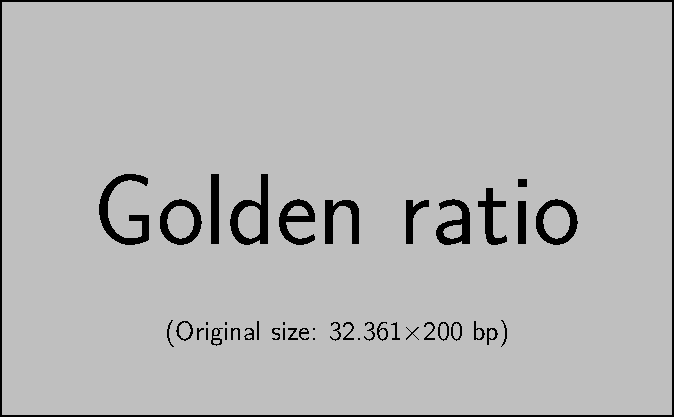
\includegraphics[width=\textwidth]{placeholder_images/example-image-golden.pdf}
    \caption[Schematic illustration depicting geometrical origins of the \gls{spm}]
    {Schematic illustration depicting the geometrical origins of the \gls{spm}. The \gls{spm} is obtained through a degenerate spatial discretisation of one electrochemical layer within a typical Li-ion pouch cell. The axial direction along the cell's thickness is denoted by $x(t)$, whilst the pseudo-dimension along the radial depth of each electrode particle is denoted by $r(t)$. In the basic \gls{spm}, the active material of each porous electrode is represented by one representative spherical particle, thus entirely eliminating the spatial dimension along the axial direction.}
    \label{fig:sandwichtospm}
\end{figure}


Figure~\cref{fig:sandwichtospm}  shows the  arrangement  of one  electrochemical
layer within a typical Li-ion pouch cell. A description of the working principle
of the  cell was presented in~\cref{ch:chapter1}  and is not repeated  here. The
\gls{spm}, as the name suggests,  models the electrochemical phenomena along the
thickness  $l_j$, \jinnegpos{}  of  each porous  electrode  by a  representative
spherical particle.  Thus the two  distinct solid-phase porous materials  of the
cell, \ie{} the  negative and positive electrodes, are idealised  as two spheres
of radii $r_\text{neg}$ and $r_\text{pos}$ respectively.


In  this  reformulated  arrangement,  the  spatial  dimension  along  the  axial
thickness  of  each  electrode  degenerates   to  a  single  point.  Hence,  the
concentration of Lithium within each electrode $c_{\text{s}_j}$, \jinnegpos{} is
only a  function of the radial  position $r_j$, \jinnegpos{} along  the depth of
their  representative  spherical  particle,  and time,  $t$.  The  surface  area
of  each representative  sphere  is  scaled appropriately,  such  that they  are
equivalent  to the  active area  of  the corresponding  porous electrodes.  Thus
the  \gls{spm} accounts  for  the  reduced volume-fraction  arising  due to  the
microporous  structure of  the solid-phase.  The overarching  assumption of  the
\gls{spm} modelling philosophy is that  the electrochemical performance of these
representative electrodes are  sufficient to model the behaviour of  the cell at
its  terminals.  The  \gls{spm}  thus  employs  the  coarsest  possible  spatial
discretisation of the cell's thickness with the goal of minimising computational
burden.


\subsection{Model Development --- Scope and Assumptions}

Having established the geometrical representation of the model, it is imperative
to establish its  aims and scope. This section discusses  the subset of physical
phenomena that can captured by the model and enumerates the inherent assumptions
in  model derivation.The  validity of  these  assumptions and  their effects  is
discussed  in~\cref{subsec:basicspmlimitations}.  As  a  broad  outline  of  the
\gls{spm}s scope,  the model  attributes the cell  polarisation to  two dominant
physics,  \viz{} reaction  kinetics and  solid-phase transport  phenomena, \ie{}
diffusion dynamics.


The gls{spm} assumes that charge transfer happens throughout the surface of each
representative  spherical particle  where intercalation  occurs. The  electronic
conductivity  of the  solid-phase is  assumed to  be high  enough to  ignore the
spatial distribution  of charge, \ie{}  the local volumetric current  density is
assumed  to be  uniform  along  the thickness  of  each  porous electrode.  This
assumption  is motivated  by  the  early calculations  performed  by Newman  and
Tobias~\cite{Newman1962} in their stand-alone  analysis of current distributions
in porous electrodes, wherein a volume-averaged molar flux is deemed sufficient.
This uniform current density assumption implies that all of the particles in the
electrode active material are in parallel.


In the  \gls{spm}, solid-phase  diffusion dynamics are  solved by  assuming this
averaged electrochemical  reaction rate.  In the simulation  study by  Smith and
Wang~\cite{Smith2006b},  it  is  reported  that, soon  after  the  beginning  of
discharge, solid-phase concentration and ionic flux become nearly independent of
spatial position, and  Lithium diffusion in solid particles may  be driven by an
averaged molar flux at the surface.


\subsection{Limitations and Drawbacks}\label{subsec:basicspmlimitations}

The modelling foundations of the \gls{spm} have been






\section{Electrolyte Inclusion}\label{sec:electrolyteinclusion}

Rahimian~\etal{}~\cite{KhaleghiRahimian2013} discuss  the usage of  a polynomial
approximation  for   electrolyte  concentration  and  potentials.   However,  no
restriction was imposed on the order  of the polynomials chosen to represent the
electrolyte concentration within  each porous electrode region.  In the standard
\gls{dfn} model, the  number of equations and  corresponding boundary conditions
describing electrolyte charge and mass transport within the cell is insufficient
to uniquely solve for all  unknown coefficients of the polynomial approximation.
The  challenges  posed  due  to  this equation  deficiency  shall  be  discussed
in~\cref{temp:eqndeficiency}. Although  the original  \gls{spm} did  not involve
solving  for  the  electrolyte  concentrations  or  potentials,  The  polynomial
approximation of the single


Rahimian~\etal{} adopted  a cubic  polynomial for approximating  the electrolyte
concentration within  the porous electrodes.  To overcome the issue  of equation
deficiency, they adapted a scheme wherein one additional spatial location in the
interior  of  each  electrode  was  used. The  coefficients  of  the  polynomial
approximation  were then  obtained  by iteratively  solving  a relatively  large
coupled  system of  algebraic equations,  embedding within  them the  additional
equations evaluated at  the interior point. An additional  complicating issue is
the specific positioning of this  additional interior point. An online numerical
optimisation  was performed  to obtain  the optimal  placement of  this interior
node. Although it serves as a proof of concept towards implementing higher order
polynomial approximations,  the author of this  thesis deems this method  as too
complex for online implementations.

\section{New Electrolyte Model}\label{sec:newelectrolytemodel}



\subsection{equation deficiency \dots}\label{temp:eqndeficiency}

% \begin{figure}[htb]
% \begin{algorithmic}[1]

% \Procedure{SUM}{ $\{x\}$}

% \State $y\gets0$
% \For{$i \gets 1 : N^{x}$} \Comment{Time series $\{x\}$ has length $N^{x}$}
%    \State $y\gets y+x(i)$ \Comment{Summing up.}
% \EndFor

% \State \textbf{return}  $y$
% \EndProcedure
% \end{algorithmic}
% \caption[Implementation of a algorithm for calculating a sum.]{Implementation of a algorithm for calculating a sum.}
% \label{fig:algorithm1}
% \end{figure}




% ---------------------------------------------------------------------------
%: ----------------------- end of thesis sub-document ------------------------
% ---------------------------------------------------------------------------



% % -*- root: ../main.tex -*-
%!TEX root = ../main.tex
% this file is called up by main.tex
% content in this file will be fed into the main document
% vim:textwidth=80 fo=cqt

In this  section, the performance  of the  basic \gls{spm} is  discussed through
desktop  simulation and  by comparison  against a  standard \gls{dfn}  benchmark
model incorporating the full \gls{p2d} dynamics.

\subsection{Cell Parametrisation}\label{subsec:spmp2dparametrisation}
% -*- root: ../main.tex -*-
%!TEX root = ../main.tex
% this file is called up by main.tex
% content in this file will be fed into the main document
% vim:nospell

\begin{table}[!htbp]
    \small
    \caption[Simulation parameters of  an \protect{\gls{lco}} cell]{Complete set
        of  parameters for  simulating the  \protect{\gls{p2d}} and  \protect{\gls{spm}}
        implementations  of an  \protect{\gls{lco}} cell  (with \ch{LiCoO_2}--\ch{LiC_6}
        electrode   pair  and   \ch{LiPF_6}   electrolyte).   The  highlighted   entries
        represent the  parameters exclusive  to \gls{p2d} model.\quad  \protect{$j \in
    \{\text{pos},\text{sep},\text{neg}\}$}}
    \label{tbl:lcoSimParamsSPMp2d}
    \vspace{-2.6229525pt}
    \begin{threeparttable}
        \centering
        \begin{varwidth}[t]{0.48\linewidth}
            \begin{tabular*}{\textwidth}{@{} l @{\extracolsep{\fill}} r @{}}
                \multicolumn{2}{c}{\textbf{System Conditions}} \\
                \toprule
                \multicolumn{1}{@{}l}{Parameter} \\
                \midrule

                Lower cutoff cell voltage, $V_\text{min}$ (\si{\volt}) & \tnote{a}2.50   \\
                Upper cutoff cell voltage, $V_\text{max}$ (\si{\volt}) & \tnote{b}4.30   \\
                Cell temperature, $T_\text{cell}$ (\si{\kelvin})       & \tnote{c}298.15 \\

                \bottomrule
            \end{tabular*}
        \end{varwidth}
        \hfill
        \begin{varwidth}[t]{0.48\linewidth}
            \begin{tabular*}{\textwidth}{@{} l @{\extracolsep{\fill}} r @{}}
                \multicolumn{2}{c}{\textbf{Other Constants}} \\
                \toprule
                \multicolumn{1}{@{}l}{Parameter} \\
                \midrule

                Faraday constant, $F$ (\si{\coulomb\per\meter})                                                        & 96487         \\
                Universal gas constant, $R$ (\si{\joule\per\mole\per\kelvin})                                          & 8.314         \\
                \textcolor{imperialblue}{\emph{Init.}}\ electrolyte conc., $c_\text{e,0}$ (\si{\mole\per\meter\cubed}) & \tnote{c}1000 \\

                \bottomrule
            \end{tabular*}
        \end{varwidth}

        \bigskip
        \vspace{-2.6229525pt}
        % \vfill

        \begin{tabular*}{\textwidth}{@{} =P{7.5cm} @{\extracolsep{\fill}} +l +c +r @{}}
            \multicolumn{4}{c}{\textbf{Thermodynamic, Kinetic, Geometric and Transport Parameters}} \\
            \toprule
            \multicolumn{1}{@{}l}{Parameter} & \multicolumn{1}{l}{Pos} & \multicolumn{1}{c}{Sep} & \multicolumn{1}{r@{}}{Neg}\\
            \midrule

            \rowstyle{\color{imperialblue}} Bruggeman coefficient, $\text{brugg}_j$                                                 & \tnote{c}\num{4}        & \tnote{c}\num{4}                               & \tnote{c}\num{4}        \\
            \rowstyle{\color{imperialblue}} Intrinsic electrolyte diffusivity, $D$ (\si{\meter\squared\per\second})               & \tnote{d}\num{3.22e-10} & \tnote{d}\num{3.22e-10}                        & \tnote{d}\num{3.22e-10} \\
            \rowstyle{\color{imperialblue}} Intrinsic electrolyte conductivity, $\kappa$ (\si{\siemens\per\meter})                &
            \multicolumn{3}{c}{\textcolor{imperialblue}{\Vhrulefill{} see table note \emph{e} \&~\cref{subsec:basicspmsimsetup} \Vhrulefill{}}}\\
            \rowstyle{\color{imperialblue}} \ch{Li^+} transference number, $t^0_\text{+}$                                           & \tnote{c}\num{0.363}    & \tnote{c}\num{0.363}                           & \tnote{c}\num{0.363}    \\
            \rowstyle{\color{imperialblue}} Intrinsic electronic conductivity, $\sigma_j$ (\si{\siemens\per\meter})                 & \tnote{c}\num{100.00}   & ---                                            & \tnote{c}\num{100.00}   \\
            Thickness, $l_j$ (\si{\meter})                                                          & \tnote{c}\num{88e-6}    & \textcolor{imperialblue}{\tnote{c}\num{25e-6}} & \tnote{f}\num{72e-6}    \\
            Electrolyte porosity, ${\varepsilon}_j$                                                 & \tnote{c}\num{0.385}    & \tnote{c}\num{0.724}                           & \tnote{c}\num{0.485}    \\
            Filler vol.\ fraction, ${\varepsilon}_{\text{fi}_j}$                                    & \tnote{c}\num{0.025}    & ---                                            & \tnote{c}\num{0.033}    \\
            Particle radius, $R_\pj$ (\si{\meter})                                                  & \tnote{c}\num{2e-6}     & ---                                            & \tnote{c}\num{2e-6}     \\
            Specific interfacial surface area, $a_\sj$ (\si{\meter\squared\per\meter\cubed})        & \tnote{g}\num{885e3}    & ---                                            & \tnote{g}\num{723.6e3}  \\
            Electrode diffusivity, $D_{\text{s}_j}$ (\si{\meter\squared\per\second})                & \tnote{c}\num{1e-14}    & ---                                            & \tnote{c}\num{3.9e-14}  \\
            Stoichiometry, 0\% SOC, ${\theta}_{\text{min}_j}$                                       & \tnote{h}\num{0.9917}   & ---                                            & \tnote{h}\num{0.0143}   \\
            Stoichiometry, 100\% SOC, ${\theta}_{\text{max}_j}$                                     & \tnote{c}\num{0.4955}   & ---                                            & \tnote{c}\num{0.8551}   \\
            Max concentration, ${c_\text{s,max}}_j$ (\si{\mole\per\meter\cubed})                    & \tnote{c}\num{51554}    & ---                                            & \tnote{c}\num{30555}    \\
            Reaction rate coefficient, $k_\jr$ (\si{\meter\tothe{2.5}\mole\tothe{-0.5}\per\second}) & \tnote{c}\num{2.33e-11} & ---                                            & \tnote{c}\num{5.03e-11} \\
            Overall active surface area, $A$ (\si{\meter\squared})                                  & \tnote{i}\num{2.053}    & ---                                            & \tnote{i}\num{2.053}    \\
            Open circuit potential, $U_j$ (\si{\volt})                                              & \tnote{k}see table note & ---                                            & \tnote{m}see table note \\
            \bottomrule
        \end{tabular*}

        \bigskip
        \vspace{-2.6229525pt}
        % \vfill
        %%%%%%%%%%%%%%%%%%%%%%%%%%%% SIMULATION PARAMS TABLE %%%%%%%%%%%%%%%%%%%%%%%%%%%%%
        \begin{tabular*}{\textwidth}{@{} =P{7.5cm}  +l@{\extracolsep{\fill}}+c +r @{}}
            \multicolumn{4}{c}{\textbf{Spatial Discretisation}} \\
            \toprule
            \multicolumn{1}{@{}l}{Parameter} & \multicolumn{1}{l}{Pos} & \multicolumn{1}{c}{Sep} & \multicolumn{1}{r@{}}{Neg}\\
            \midrule

            \rowstyle{\color{imperialblue}} Nodes, through-thickness (axial), $N_{\text{a}_j}$          & \num{15} & \num{15} & \num{15} \\
            \rowstyle{\color{imperialblue}} Nodes, within spherical particle (radial), $N_{\text{r}_j}$ & \num{10} & ---      & \num{10} \\

            \bottomrule
        \end{tabular*}

        \medskip
        \vspace{-2.6229525pt}
        % \vfill
        \begin{tablenotes}[para,flushleft]
            \begin{scriptsize}
            \item[a] Ref.~\cite{Northrop2011}
            \item[b] Set to $\approx $\SI{100}{\milli\volt} above the cell's \gls{ocp} at \SI{100}{\percent} cell \gls{soc}
            \item[c] Ref.~\cite{Subramanian2009}
            \item[d] Computed at $T_\text{cell} = \SI{298.15}{\kelvin}$ using coefficients from table \rom{2} in Ref.~\cite{Valoen2005}\\%\fxnote{cross-ref to actual equation}
            \item[e] Computed at $T_\text{cell} = \SI{298.15}{\kelvin}$ using coefficients from table \rom{3} in Ref.~\cite{Valoen2005} at $c_\text{e,0}= \SI{1000}{\mole\per\meter\cubed}$\\
            \item[f] Set up for capacity balance of electrodes such that $l_\text{neg} = 1.22 \times l_\text{pos}$ here.
            \item[g] Computed as per~\cref{eq:specificsurfarea}\\
            \item[h] Obtained as residual stoichiometries after a C/\num{500} simulated discharge from \SI{100}{\percent} cell \gls{soc} to \SI{2.7}{V}
            \item[i] Chosen so that current density for the electrochemical layer is \SI{29.23}{\ampere\per\meter\squared} for \SI{60}{\ampere} applied current
            \end{scriptsize}
            \vspace{1ex}
            \item[k] $ \mathcal{U(\theta_\text{pos})} = \textstyle \frac{-4.656 + 88.669\theta_\text{pos}^2 - 401.119\theta_\text{pos}^4 + 342.909\theta_\text{pos}^6 - 462.471\theta_\text{pos}^8 + 433.434\theta_\text{pos}^{10}}{-1 + 18.933\theta_\text{pos}^2 - 79.532\theta_\text{pos}^4 + 37.311\theta_\text{pos}^6 - 73.083\theta_\text{pos}^8 + 95.96\theta_\text{pos}^{10}}$ \\[0.25em]
            \begin{footnotesize}
            \item[m] $\mathcal{U(\theta_\text{neg})} = 0.7222 + 0.1387\theta_\text{neg} + 0.029\theta_\text{neg}^{0.5} - \frac{0.0172}{\theta_\text{neg}} + \frac{0.0019}{\theta_\text{neg}^{1.5}} + 0.2808 e^{(0.9 - 15\theta_\text{neg})} - 0.7984 e^{(0.4465\theta_\text{neg} - 0.4108)}$\vfill
            \end{footnotesize}
        \end{tablenotes}
    \end{threeparttable}
\end{table}

% Electrolyte diffusivity, $D_j$ \si{(m^2.s^{-1})}                         & \multicolumn{3}{c} {\Vhrulefill{} refer to equation in \tnote{g} \Vhrulefill{}} \\
% \item[g] $ D_j = 10^{-4} \times 10^{-4.43 - \frac{54}{T_\text{cell} - 229 - 5\times10^{-3} c_\text{e}(x,t)} - 0.22\times10^{-3} c_\text{e}(x,t)}, \quad \jinpossepneg $\\

% $\scriptstyle 10^{-4} c_\text{e} \left(-10.5 + \num{0.668e-3} c_\text{e} + \num{0.494e-6} c_\text{e}^2 + (0.074 - \num{1.78e-5}) c_\text{e} - \num{8.86e-10} c_\text{e}^2\right)T_\text{cell} + \left(\num{-6.96e-5} + \num{2.8e-8} c_\text{e})T_\text{cell}^2\right)^2$
% \tnote{e}\num{26.24e-3} & \tnote{e}\num{328.15e-3}                       & \tnote{e}\num{66.08e-3} \\


\Cref{tbl:lcoSimParamsSPMp2d} lists  the simulation  parameters of  an \gls{lco}
cell  whose positive  and negative  electrodes are  \ch{LiCoO_2} and  \ch{LiC_6}
respectively.  The  electrolyte in  this  system  consists of  \ch{LiPF_6}  salt
in  a   solution  of   \gls{ec}/\gls{dmc}/\gls{emc}  in   a  1:1:1   ratio.  The
standard  set  of  \gls{dfn}  parameters have  been  extensively  described  and
documented  in  literature.  The   detailed  characterisation  of  the  physical
properties  of  lithium-ion  cells  falls  outside the  scope  of  this  thesis.
Here, the  vast majority  of electrochemical  parameters, \viz{}  the geometric,
thermodynamic, kinetic  and transport properties  of the cell have  been sourced
from  Subramanian~\etal{}~\cite{Subramanian2009}.   The  significance   of  each
of  the  parameters  in  the  context of  the  modelling  assumptions  discussed
in~\cref{subsec:basicspmassumptions} is examined.


The simulation parameters that are applicable exclusively to the \gls{p2d} model
are shown as  highlighted text in~\cref{tbl:lcoSimParamsSPMp2d}. It  can be seen
that only a  subset of the isothermal \gls{dfn} model's  parameters are required
for the the \gls{spm}. In particular, there is no requirement to estimate any of
the electrolyte-related  parameters in  each electrode region.  Furthermore, the
properties of the separator material which  are necessary in the \gls{dfn} model
are also  not considered in the  \gls{spm} computations. A brief  enumeration of
the additional  \gls{p2d}-specific parameters in the  context of parametrisation
requirements is provided here.

\begin{enumdescriptnum}[leftmargin=!,itemsep=1ex,labelwidth=\widthof{$\symbf{\text{brugg}_j}\ \scriptstyle (\times 3)$abc}
    ,partopsep=0pt
    ,topsep=0pt
    ]

    \customenum{\text{brugg}_j}{3}  The  empirical Bruggeman  coefficient  helps
    to   define   the  effective   values   of   conductivity  and   diffusivity
    of   the  electrolyte.   Although  an   identical   value  of   4  is   used
    in~\cref{tbl:lcoSimParamsSPMp2d}, in  principle all  three regions  can have
    different values of brugg and need to be parametrised separately.

    \customenum{D}{1}  The  intrinsic  electrolyte   diffusivity  of  a  typical
    electrolyte  consisting  of  \ch{LiPF_6}  salt in  an  organic  solvent  was
    experimentally  characterised   and  provided  as  a   table  of  polynomial
    coefficients  by  Valøen  and  Reimers~\cite{Valoen2005}.  Evaluating  this
    polynomial  at a  cell  temperature of  \SI{298.15}{\kelvin}  results in  an
    intrinsic diffusivity of \SI{3.22e-10}{\meter\squared\per\second}. Since the
    intrinsic  diffusivity is  a material  property  and is  independent of  the
    region within the cell, it needs to be parametrised only once.

    \customenum{\scalebox{1.35}{$\kappa$}}{1}   Like    the   diffusivity,   the
    intrinsic electrolyte conductivity is also a material property and its value
    is independent  of the region within  the cell. Unlike the  diffusivity, the
    electrolyte conductivity  is a strong  function of its  ionic concentration.
    Thus, the polynomial proposed by Valøen and Reimers~\cite{Valoen2005} needs
    to  be evaluated  at  $T_\text{cell}= \SI{298.15}{\kelvin}$  and  has to  be
    updated during the  simulation as salt concentration  within the electrolyte
    changes over time. A discussion on the choice of initial concentration is
    provided in~\cref{subsec:basicspmsimsetup}.

    \customenum{\scalebox{1.25}{$t$}_+^0}{1}  The  cationic transference  number
    measures the relative  mobility of the \ch{Li^+} ion in  the organic solvent
    and is  independent of  the region  within the  cell. Hence,  this intrinsic
    property is to be parametrised only once (per solvent).

    \customenum{\scalebox{1.25}{$\sigma$}_j}{2} The intrinsic conductivity of the solid
    phase depends on the material used in the porous electrodes. Although a
    simplified assumption of equal conductivity is used for the two electrodes,
    in practice, this property needs to be characterised for each of the two
    electrodes.

\end{enumdescriptnum}

\sisetup{detect-weight=true}   Thus,   neglecting   Arrhenius-type   temperature
dependence of  physical properties and their  corresponding activation energies,
the basic  \gls{spm} facilitates the  ability to afford  physics-based modelling
capabilities with  \emph{eight} fewer parameters than  the equivalent isothermal
\gls{p2d} model. With  the naive assumption of equal  parametrisation effort per
physical property, this  implies a \textbf{\SI{20}{\textbf{\percent}}} reduction
in  parametrisation  requirements  for  the basic  \gls{spm}  when  compared  to
its  \gls{dfn} counterpart.  However,  considering the  fact that  parametrising
the  electrolyte's transport  properties requires  apparatus and  infrastructure
typically available  only in specialised chemical/materials  labs, the reduction
in parametrisation  overhead for  system-level engineering stakeholders  is more
pronounced.

Prima facie, it may seem that electrolyte porosities and filler volume fractions
do  not  influence the  \gls{spm}  model.  However,  they  do have  an  indirect
bearing  on arriving  at a  critical parameter,  \viz{} the  solid phase  volume
fraction, $\varepsilon_\sj$. This parameter is  required to compute the specific
interfacial  surface  area  of  the  electrodes  $a_\sj$,  \ie{}  the  effective
electrode area exposed  to reaction and is an important  entity in the \gls{spm}
model  equations  presented  in~\cref{subsec:basicspmgoverningeqns}.  The  solid
phase volume fractions are also required in simulating the \gls{p2d} model owing
to  the  need for  computing  the  effective  electronic conductivities  of  the
electrodes.\fxnote{cross-reference to  specifc newman equations here}.  They are
calculated as
\begin{equation}
    \varepsilon_\sj = 1 - \varepsilon_j - \varepsilon_{\text{fi}_j}
\end{equation}
where $\varepsilon_j$  and $\varepsilon_{\text{fi}_j}$  are the  electrolyte and
filler  volume-fraction  within  the  respective electrode  regions.  Using  the
values from~\cref{tbl:lcoSimParamsSPMp2d} results in $\varepsilon_\spos = 0.590$
and  $\varepsilon_\sneg  =  0.482$  for the  positive  and  negative  electrodes
respectively. The specific interfacial surface areas are then calculated as
\begin{equation}\label{eq:specificsurfarea}
    a_\sj = \varepsilon_\sj \frac{4 \pi R_\pj^2}{\frac{4}{3} \pi R_\pj^3} = \frac{3\varepsilon_\sj}{R_\pj}
\end{equation}

As    discussed   in    the   assumptions    made   during    model   derivation
(see~\cref{subsec:basicspmassumptions})  and consistent  with the  assumed model
geometry,  the  parameters  not  covered  by  the  \gls{spm}  pertain  to  those
describing electrolyte dynamics and distribution  of electronic charge along the
axial  thickness  direction  of  the  cell. Properties  such  as  the  intrinsic
diffusivities  and conductivities  of  the electrolyte,  transference number  of
\ch{Li^+} in  the organic  solvent are thus  completely redundant  for \gls{spm}
simulation. The assumption of uniform charge density along the through-thickness
length of each electrode implies that the intrinsic electronic conductivities of
the two electrodes  do not play any  role in the model  dynamics. The porosities
and Bruggeman  coefficients in~\cref{tbl:lcoSimParamsSPMp2d} serve  as modifying
factors  of  the  intrinsic  conductivities  and  diffusivities  leading  to  an
effective value  within each  region of the  electrochemical layer.  Thus, their
relevance is also  rendered void in the case of  the basic \gls{spm} simulation.
The  thickness of  the  separator  material only  plays  a  role in  electrolyte
behaviour.  By the  model geometry  presented in~\cref{subsec:basicspmgeometry},
this parameter also falls outside the scope of the basic \gls{spm}.

The  thicknesses  of the  electrodes  are  optimised  for equal  loading,  \ie{}
to  achieve  a   balance  in  their  individual  capacities   to  store  \ch{Li}
atoms.  The thickness  of the  positive  electrode is  the chosen  as the  value
from~Subramanian~\etal{}~\cite{Subramanian2009}. The  thickness of  the negative
electrode region  is then  computed with  the goal of  equalising the  volume of
active material  in each electrode  for every  electrochemical layer in  a pouch
cell.
\begin{equation}\label{eq:basiccapacitybalance}
    A_{\text{elec}_\text{pos}}\varepsilon_\spos l_\text{pos} = A_{\text{elec}_\text{neg}}\varepsilon_\sneg l_\text{neg}
\end{equation}

In a  lithium-ion pouch cell, the  electrodes are designed such  that the layers
can be  overlaid on  top of  one another  and finally  encapsulated in  a pouch.
Geometrical considerations  then imply  that the  cross-sectional area  (or face
area) of the two electrodes must be  the same. However, due to the consideration
of  avoiding  plating  at  the  edges  due  to  microscopic  malformations,  the
design  is done  such as  to have  a small  overhang of  the negative  electrode
layer,  \approx\SI{2}{\milli\meter}  with  respect  to  the  positive  electrode
layer\fxnote{citation  needed}  as  shown  in~\cref{fig:anodeoverhangpouchcell}.
However, the  active surface area, is  just the common overlap  area between the
two electrodes, and  thus, $A_\text{elec}$ is equal to  the cross-sectional area
of the positive electrode.

\begin{figure}[!htb]
    \centering
    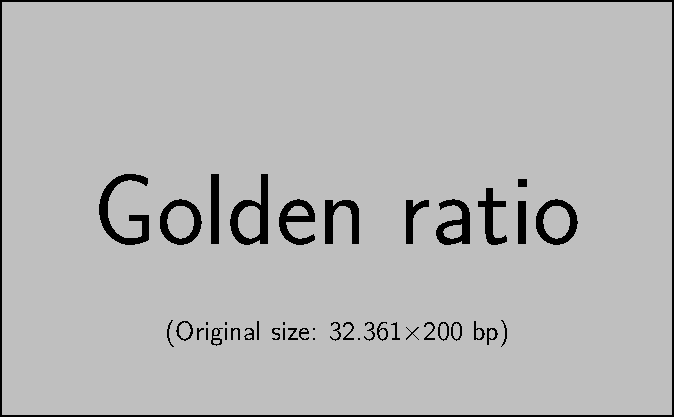
\includegraphics{placeholder_images/example-image-golden.pdf}
    \caption[Stacking of layers within a pouch cell]
    {Image showing the stacking of layers within a pouch cell. For the negative
        electrodes, there is a small overhang (\approx\SI{2}{mm}) at the
        edges with respect to the positive electrodes. This design choice
    helps to avoid plating of lithium at the edges.}
    \label{fig:anodeoverhangpouchcell}
\end{figure}

Thus,~\cref{eq:basiccapacitybalance} reduces to
\begin{equation}
    \frac{l_\text{neg}}{l_\text{pos}} = \frac{\varepsilon_\text{pos}}{\varepsilon_\text{neg}} = 1.22
\end{equation}
yielding $l_\text{neg} = \SI{72}{\micro\meter}$.

At first, it  may be surprising to  note that the values of  the particle radius
$R_\pj$ used in  both the \gls{p2d} and \gls{spm} remain  identical. However, it
is important  to note that  the \gls{p2d} equations  of the \gls{dfn}  model are
cast in  a normalised  form, \ie{}  already set  up to  account for  the overall
capacity of the  cell under consideration implicitly through usage  of a current
density  (per unit  area) for  its  simulation. Furthermore,  this explains  why
increasing the  number of  discretisation nodes does  not increase  the modelled
capacity, but  instead serves to improves  the simulation accuracy owing  to the
enhanced spatial resolution.

The  overall  active  surface  area  $A  =  n  A_\text{elec}$  is  the  combined
cross-sectional  area  of all  layers  ($n$  is  the number  of  electrochemical
(pos,sep,neg)  triplets) stacked  into the  pouch  cell. In  both the  \gls{p2d}
and  \gls{spm}  models,  this  parameter  serves  to  scale  the  external  load
current  down  to  the  current  density  experienced  by  each  electrochemical
layer. A value of  \approx\SI{30}{\ampere\per\meter\squared} was reported in the
results section of  Subramanian~\etal{}~\cite{Subramanian2009}. When considering
a \SI{60}{\ampere\hour} pouch cell with \SI{10}{\milli\meter} exterior thickness
and  using  the  parameters  reported  in~\cite{Subramanian2009},  this  results
in  a cross-sectional  area of  \SI{2.053}{\meter\squared}\fxnote{to add:  refer
to  layer  optimisation  chapter   for  detailed  derivation}.  Considering  the
equalisation of capacity  loading, with the newly chosen thickness  value of the
negative  electrode, the  1C-rate  capacity  of the  cell  has  been revised  to
\SI{29.23}{\ampere\per\meter\squared}.

On  simulating  the \gls{p2d}  model  with  a  trickle bleeding  type  discharge
corresponding   to   a  current   of   C/500   and   logging  the   data   every
\SI{1}{\milli\second}, after reaching \SI{2.7}{\volt}\footnote{From manufacturer
    datasheets  for \protect{\gls{lco}}  chemistries,  this value  is considered  to
correspond to \SI{0}{\percent} \protect{\gls{soc}}.}, the remnant concentrations
in  the two  electrodes  were noted.  The  corresponding residual  stoichiometry
values  are reported  in~\cref{tbl:lcoSimParamsSPMp2d}  and  is consistent  with
typical values reported in literature for \gls{lco} chemistries.\fxnote{citation
needed here.}  This validation is  important, since below  certain stoichiometry
thresholds, the spinel/olivine  structure of the electrodes  can become unstable
and  collapse\fxnote{citation needed?}.

Since   the   cell   behaviour   is   considered   isothermal,   the   parameter
table     in~\cref{tbl:lcoSimParamsSPMp2d}     omits     activation     energies
for    the   various    diffusivities    and    conductivities   of    materials
(see~\cref{subsec:basicspmsimsetup}  for  further thermal  considerations).  For
this  reason,~\cref{tbl:lcoSimParamsSPMp2d}  does  not  include  other  material
properties such  as specific  heats, and  thermal conductivities.  No properties
of  the  current  collectors  appear  in  the  isothermal  model  equations  for
both  the \gls{p2d}  and  \gls{spm}  models and  hence  are  omitted. All  other
electrochemical  properties,   \viz{}  stoichiometries   at  \SI{100}{\percent},
maximum concentrations, diffusivities, reaction  rate coefficients and \gls{ocp}
of  the two  electrodes remain  invariant  between the  \gls{p2d} and  \gls{spm}
models.

\subsection{Simulation Setup}\label{subsec:basicspmsimsetup}

For  reproducibility of  results, it  is important  to discuss  the system-level
parameters influencing simulation setup.

The  lower cutoff  voltage of  the cell  is chosen  to be  \SI{2.5}{\volt}. This
is  deliberately  kept  lower  than  the voltage  corresponding  to  the  cell's
\SI{0}{\percent},  \ie{}  \SI{2.7}{\volt}.  If set  above  \SI{2.7}{\volt}  even
at  infinitesimally small  discharge  currents, the  cell  would cut-off  before
achieving complete discharge. Choosing a value lower than \SI{2.7}{V} means that
the cell gets a chance to recover its terminal voltage, despite spikes in highly
dynamic  load  currents  that  might  bring the  voltage  below  this  threshold
momentarily. If a low-enough value is  not chosen, a system-level shutdown shall
be  initiated  despite possessing  the  ability  to  continue to  operate  after
recovery  of terminal  voltage.  In  this case,  choosing  a  cutoff voltage  of
\SI{2.5}{\volt}  does  not  damage  the  cell  since  checks  are  in  place  to
monitor  the \gls{soc}  and  trigger cutoff  in the  event  of charge  depletion
(see~\cref{alg:ctstimespm,alg:disctimespm}).  Northrop~\etal~\cite{Northrop2011}
use this value, although no explanation is given for the choice.

The  upper  cutoff voltage  of  the  cell  is  chosen at  \SI{4.3}{\volt}  \ie{}
\approx\SI{100}{\milli\volt}   higher   than   the  equilibrium   \gls{ocp}   at
\SI{100}{\percent} \gls{soc}. There are several  reasons for this smaller margin
at the upper end of the voltage spectrum
\begin{description}[leftmargin=!,labelwidth=\widthof{\bfseries low
    probabilities},itemsep=1ex]

\item[safety] li-ion  cells are less  tolerant to overcharging and  can pose
    fire hazards.

\item[degradation]  overcharging  li-ion  cells  can  lead  to  plating  and
    accelerate other degradation mechanisms.

\item[low  C-rates]  charging C-rates  are  typically  lower than  discharge
    C-rates.

\item[CCCV charging]  For on-board  chargers, taper charging  (such as  in a
    \gls{cccv} profile) is activated, which  ensures that charging current drops
    off  rapidly, leading  to a  lower overvoltage  towards the  upper \gls{soc}
    range.

\item[low probabilities] The only charging event when an electrified vehicle
    is in motion is during regenerative braking. The vehicular \gls{bms} manages
    the operating window such that the starting \gls{soc} is much lower than the
    overvoltage  that  could  be  caused due  to  braking.  Furthermore,  during
    operation, the net discharge events  occur more frequently than regenerative
    braking events.

\end{description}

For  both the  \gls{p2d} model  and the  \gls{spm} model,  the cell  temperature
is   kept   constant   at   its   initial   value   of   \SI{25}{\degreeCelsius}
(\SI{298.15}{\kelvin}). This implies that the  operation of the lithium ion cell
is assumed  to be isothermal.  While this  is not true  in general, it  is worth
noting that thermal gradients in  the through-thickness direction is negligible.
\fxnote{citation needed} Furthermore, for  the C-rates considered (<5C), typical
in a \gls{bev} application and  for short-duration transient loads studied, this
is a reasonable assumption. Detailed modelling of thermal dynamics is not within
the scope of this thesis, as the primary goal is to obtain a physics based model
incorporating  electrochemical  principles  amenable for  embedded  application.
Thus, thermal dependence of parameters through an Arrhenius-type relationship is
not  considered.    Future   work  could   include  performing   thermally  coupled
simulations, incorporating  thermally relevant  parameters and use  a simplified
heat generation expression,  \eg{} a lumped thermal model in  both the \gls{spm}
and \gls{p2d} and compare their performances.

To  understand  the parametrisation  of  initial  concentration, the  expression
for   electrolyte   conductivity   needs    to   be   examined.   As   discussed
in~\cref{subsec:spmp2dparametrisation}, the intrinsic conductivity of a specific
type  of  electrolyte  is  a  material   property  that  depends  on  the  local
concentration of \ch{Li^+} ions and  temperature. In the characterisation of the
electrolyte in Valøen and  Reimers~\cite{Valoen2005}, the polynomial expression
in~\cref{eq:kappavsCeandT} was obtained for the electrolyte conductivity.
\begin{multline}\label{eq:kappavsCeandT}
    \kappa_j(c_\text{e},T)(x,t) =  10^{-4} c_\text{e}(x,t) \bigl(-10.5 + \num{0.668e-3} c_\text{e}(x,t) + \num{0.494e-6}  c_\text{e}{(x,t)}^2\\
    + (0.074 - \num{1.78e-5}) c_\text{e}(x,t) - \num{8.86e-10} c_\text{e}{(x,t)}^2 \bigr)T(t)\\
	+ \left(\num{-6.96e-5} + \num{2.8e-8} c_\text{e}{(x,t)})T(t)^2\right)^2
\end{multline}

\begin{figure}[!htb]
    \centering
    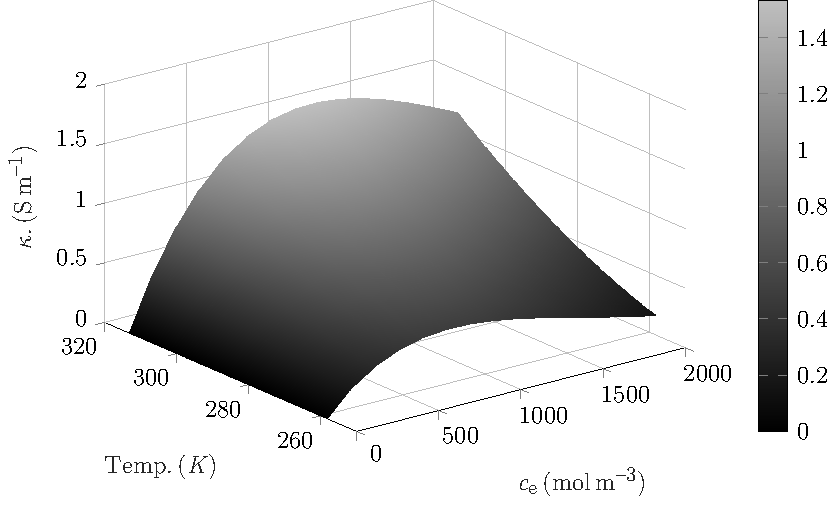
\includegraphics{4/figures/m2t_kappa_ce_T.pdf}
    \caption[Surface plot of electrolyte conductivity]
    {Electrolyte conductivity as a function of cell temperature and initial
        concentration. The variation of conductivity versus these factors is a
    smooth function.}
    \label{fig:kappavsCeandT}
\end{figure}

\Cref{fig:kappavsCeandT} shows  a surface  plot of the  electrolyte conductivity
as  a function  of  initial concentration  $c_\text{e,0}$  and cell  temperature
$T_\text{cell}$.\fxnote{comment on how the variation in the direction of temp is
less significant to that around conc} In particular,
\begin{enumerate}%[label=\emph{\alph*})]
    \item At  equilibrium  initial condition ($t=0$), $c_\text{e}$ is uniform over the axial space $x$ and
    \item only isothermal cell behaviour is considered, \ie{} $T(t) = T_\text{cell}$.
\end{enumerate}
Hence,~\cref{eq:kappavsCeandT} reduces to
\begin{multline}\label{eq:kappavsCeinitandTcell}
    \kappa_j =  10^{-4} c_\text{e,0} \bigl(-10.5 + \num{0.668e-3} c_\text{e,0} + \num{0.494e-6}  c_\text{e,0}^2\\
        + (0.074 - \num{1.78e-5}) c_\text{e,0} - \num{8.86e-10}
    c_\text{e,0}^2 \bigr)T_\text{cell}\\
	+ \left(\num{-6.96e-5} + \num{2.8e-8} c_\text{e,0})T_\text{cell}^2\right)^2
\end{multline}
As   inferred   from~\cref{fig:kappavsCeandT},  the   electrolyte   conductivity
$\kappa$   is   a  smooth   function   of   $c_\text{e}$  and   $T_\text{cell}$.
Thus~\cref{eq:kappavsCeinitandTcell}  can be  effectively  visualised through  a
parametric plot of $\kappa$ vs  $c_\text{e}$ with $T_\text{cell}$ as the varying
parameter as seen in~\cref{fig:kappavsce}.

\begin{figure}[!htb]
    \centering
    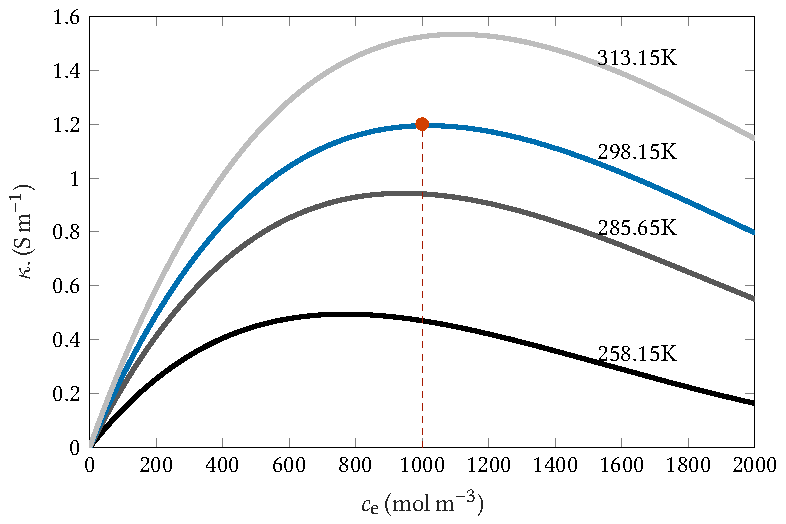
\includegraphics{4/figures/m2t_kappa_ce_parametric_T.pdf}
    \caption[]
    {Electrolyte conductivity versus equilibrium concentration at various cell
        temperatures. At ${T_\text{cell} = \SI{298.15}{\kelvin}}$, the maximum
        value of electrolyte conductivity corresponds to a salt concentration of
    \SI{1000}{\mol\per\meter\cubed}.}
    \label{fig:kappavsce}
\end{figure}

From~\cref{fig:kappavsce},       it        is       evident        that       at
$T_\text{cell}=\SI{298.15}{\kelvin}$,   the   maximum   value   of   electrolyte
conductivity is attained at  $c_\text{e} = \SI{1000}{\mole\per\meter\cubed}$. It
is advantageous  to operate  the cell  around this salt  concentration so  as to
minimise  the  cell's  overall  resistance.  Hence,  the  initial  concentration
$c_\text{e,0}$ is  chosen to  be \SI{1000}{\mole\per\meter\cubed}. It  should be
noted that while  the electrolyte concentration in the  \gls{p2d} model exhibits
both spatial  and temporal  variations during the  simulation, in  the \gls{spm}
model, it remains constant throughout.

The      reduction      in      parametrisation      requirements      discussed
in~\cref{subsec:spmp2dparametrisation}    is   only    one   of    the   factors
contributing  to   the  simplicity   and  ease   of  simulation.   As  discussed
in~\cref{subsec:basicspmgeometry},   an   important  computational   requirement
that   is  present   in   the  \gls{p2d}   model,   but  completely   eliminated
from  the   \gls{spm}  is  the   requirement  of  discretisation.   As  reported
in~\cref{tbl:lcoSimParamsSPMp2d},  with  15 nodes  per  region  along the  axial
direction  and  with 10  shells  per  electrode  in  the radial  direction,  the
\gls{p2d}  model under  simulation  achieves mesh  independence  to a  tolerance
of  \approx   \SI{2}{\percent}  for  the   range  of  C-rates   considered.  For
higher  C-rates,  coupling  a  thermal   model  is  of  higher  importance  than
incorporating further meshing refinements. The discretisation-related parameters
are  specific to  the  \gls{p2d}  model and  is  hence, highlighted  accordingly
in~\cref{tbl:lcoSimParamsSPMp2d}.

With  the cell  parametrisation discussed  and the  simulation setup  presented,
the  simulation   results  are  fully   reproducible  and  are   presented  next
in~\cref{subsec:simresultsbasicspm}.

\subsection{Simulation Results}\label{subsec:simresultsbasicspm}

\subsubsection*{Capacity Characterisation}\label{subsubsec:capcharspmp2d}

First,  it  must be  established  that  incorporating the  parameters  presented
in~\cref{tbl:lcoSimParamsSPMp2d} into the \gls{spm} model equations results in a
cell with  \emph{identical} capacity as the  \gls{dfn} model. This is  to ensure
the  validity  of  comparisons  in  further simulations.  Using  the  values  of
per-layer  C-rate as  discussed  in~\cref{subsec:spmp2dparametrisation} and  the
overall active  surface area from~\cref{tbl:lcoSimParamsSPMp2d}, the  cell under
simulation has a capacity of \SI{60}{\amphour}.

Present literature  in battery modelling, both  for the \gls{dfn} model  and for
the  \gls{spm}  do not  discuss  any  aspect  of capacity  characterisation.  In
particular, parameters such  as as the geometric surface area  of cells and even
their  1C-rate are  often  not  listed in  publications.  This  practice can  be
attributed  to the  fact that  all one-dimensional  and \glsfmtlong{p2d}  models
operate on  a per-layer basis, using  an applied current \emph{density}.  Many a
time,  researchers assume  a  unit  surface area  for  the  cell. This  implicit
normalisation  is amenable  to  those  studies which  strive  to make  numerical
comparisons between  models through simulation. However,  it leads to a  lack of
clarity on  the actual capacity of  the cells being modelled.  Furthermore, when
comparing with experimental  data from a real cell, such  works resort to ad-hoc
techniques such as empirical curve-fitting for obtaining the surface area. Often
the source  of such parametrisation  is not made  clear. Chapter~\cref{ch:layer}
documents  the details  of  obtaining  the overall  surface  area  of cells  and
arriving  at the  C-rate per  layer of  the specific  cell under  consideration.
Since  the \gls{dfn}  model does  not explicitly  model the  cell capacity,  the
author  is  compelled  to  provide  an exposition  on  how  a  simple  numerical
characterisation for determining cell capacity given a \emph{complete} parameter
list. \fxnote{citations needed for each accusation.}

For experimental capacity characterisation of cells, the standard practice is to
apply a very small discharge  current beginning at \SI{100}{\percent} \gls{soc},
logging the charge passed using a  high-precision coulomb counter until the cell
hits the voltage corresponding to \SI{0}{\percent} \gls{soc} as specified in the
manufacturer datasheet. In  order to decouple the effect of  the cell's dynamics
from its  capacity, it is  required to  apply an infinitesimal  bleeding current
(tending towards, but should not reach \SI{0}{\ampere}).

Current sensors in battery cycler equipment use high-precision (typically 15--18
bit) \glspl{adc}  and are  able to  offer high  \glspl{snr} except  at ultra-low
currents. The main difficulty with using very low C-rates is that it drastically
slows down the  characterisation procedure. Using a discharge  current of C/100,
\ie{}  \SI{0.6}{\ampere} in  this case,  results in  a characterisation  time of
\SI{100}{\hour} or \approx $4\sfrac{1}{4}$  days (excluding soak-times and other
set-up related  activities). Furthermore, for accurate  coloumb-counting, a high
data logging  rate is needed,  resulting in  large file sizes  and corresponding
difficulties in post-processing them.  Considering moderate buffer-sizes used in
data logging modules of typical  cell-cycler software (shared between channels),
and  to  avoid  excessively  large wait-times  for  characterisation,  discharge
currents of C/20--C/25 are usually deemed sufficient.

In order to validate  that the choice of model parameters  result in an intended
capacity  of  \SI{60}{\amphour},  an  analogous  procedure  is  carried  out  by
means  of  computer  simulation.  A  characterisation  simulation  beginning  at
\SI{100}{\percent} \gls{soc}  with a discharge current  of \SI{0.6}{\ampere} was
performed\footnote{All simulations  were performed  on a  64-bit Hewlett-Packard
Z840  workstation with  a 16-core  \text{Intel}\textsuperscript{\textregistered}
Xeon\textsuperscript{\textregistered} E5-2640 v3  (Haswell) processor clocked at
a base frequency of \SI{2.60}{\giga\hertz} with \SI{128}{\giga\byte} DDR4 RAM at
1866 MT/sec.}. If the assumed cell  capacity is indeed consistent with the model
parameters, then  this corresponds  to a  C-rate of  1/100. Therefore,  both the
\gls{p2d} and \gls{spm}  should run for exactly 100 hours  before cut-off due to
charge depletion.

% -*- root: ../main.tex -*-
%!TEX root = ../main.tex
% this file is called up by main.tex
% content in this file will be fed into the main document

\begin{table}[!htb]
    \centering
    \caption[Simulation data --- capacity characterisation of \glsfmtshort{p2d} and \glsfmtshort{spm} models]{Simulation data --- capacity characterisation of \glsfmtshort{p2d} and \glsfmtshort{spm} models. The \glsfmtshort{p2d} model is taken as the benchmark. Hence, modelling error is defined as \protect{$\varepsilon = V_\text{cell,p2d} - V_\text{cell,spm}$}.}
    \label{tbl:charSimspmp2d}
    \begin{tabular}{@{} l r r @{}}
        \toprule
        Parameter                                                       & Value  & Units              \\
        \midrule
        Data-logging interval                                           & 50.00  & \si{\milli\second} \\
        Total RAM used                                                  & 603.90 & \si{\mega\byte}    \\
        \glsfmtshort{p2d} run-time                                      & 99.94  & \si{\hour}         \\
        \glsfmtshort{spm} run-time                                      & 99.90  & \si{\hour}         \\
        \glsfmtshort{p2d} discharge capacity                            & 59.96  & \si{\amphour}      \\
        \glsfmtshort{spm} discharge capacity                            & 59.94  & \si{\amphour}      \\
        Max error, $\varepsilon_\text{max}$                             & -94.30 & \si{\milli\volt}   \\
        \glsfmtshort{rms} error, $\varepsilon_\text{\glsfmtshort{rms}}$ & 8.20   & \si{\milli\volt}   \\
        \glsfmtshort{mae} error, $\varepsilon_\text{\glsfmtshort{mae}}$ & 3.20   & \si{\milli\volt}   \\
        \bottomrule
    \end{tabular}
\end{table}


Capacity validation through computer simulation  is not bound by the limitations
of the experimental approach discussed earlier. Using 64-bit IEEE floating point
arithmetic, quantities as low as $\mathcal{O}(10^{-16})$ can be safely computed,
nullifying  any \gls{snr}  issues. \Cref{tbl:charSimspmp2d}  summarises the  key
data  from  this  simulation  run.  For  accurate  coulomb  counting,  the  data
logging  interval  is set  to  \SI{50}{\milli\second}.  Both the  \gls{p2d}  and
\gls{spm} model ran close to 100~hours.  The small deviations from this expected
termination  time  can  be attributed  to  the  fact  that  the current  is  not
arbitrarily small with  the pragmatic goal of obtaining results  in a reasonable
time. As seen in~\cref{tbl:charSimspmp2d}, even  the \emph{combined} CPU time to
simulate both  the \gls{p2d}  and \gls{spm}  models is  two orders  of magnitude
lower than  real-time. The only  issue that remains to  be addressed is  that of
considerable memory and  storage requirements due to  high-rate data-logging for
accurate coulomb counting. For a standard computer workstation, this places only
a minor  demand on  its CPU.  For comparable volume  of data  to be  logged, the
reliability  and ruggedness  of  a  dedicated workstation  far  exceeds that  of
real-time cell cyclers, thereby establishing numerical simulation as an amenable
method for characterisation of cell capacity. A major disadvantage of simulation
based capacity validation  is its extreme sensitivity to parameters  such as the
maximum concentration  of the  electrodes and  their stoichiometries,  which are
generally difficult to characterise. In this context, the experimental procedure
of  high-precision  coulomb counting  assumes  a  practical significance  as  it
requires no  knowledge of  the cell's parameters  other than  the manufacturer's
datasheet.

\begin{figure}[!htb]
    \centering
    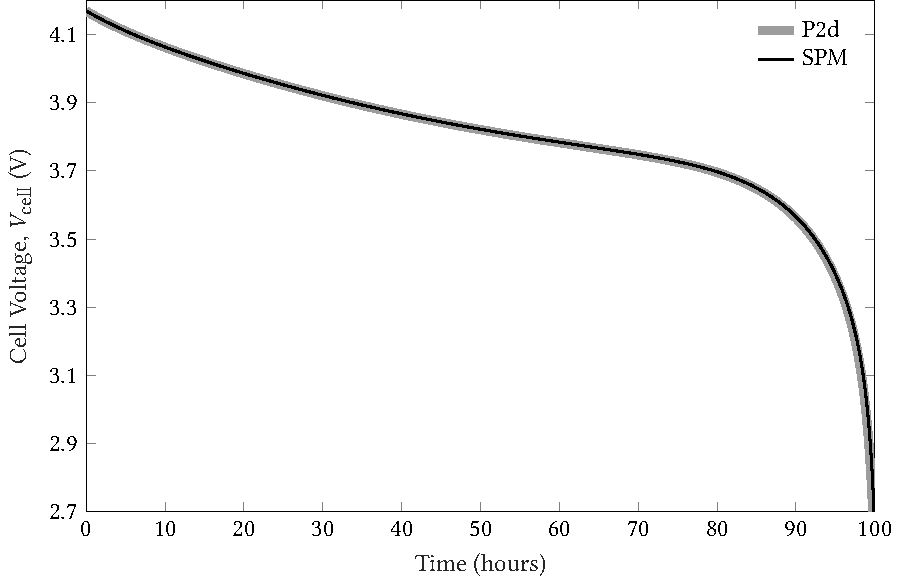
\includegraphics{4/figures/capacity_match_spm_p2d.pdf}
    \caption[Voltage response of \glsfmtshort{spm} \& \glsfmtshort{p2d} models
    for capacity validation]{Voltage response of \gls{p2d} and \gls{spm} models
        to a discharge current input of \SI{0.6}{A}. Both models achieve their
        charge depletion point after \approx\SI{100}{\hour} confirming that
        their modelled capacities match. Key simulation data for this
    characterisation run is shown in~\cref{tbl:charSimspmp2d}.}
    \label{fig:capcharspmp2d}
\end{figure}

\Cref{fig:capcharspmp2d}  shows  the  voltage  response  of  the  \gls{spm}  and
\gls{p2d}  models,  which   overlap.  It  is  clear  that   both  the  \gls{p2d}
and  \gls{spm}  models   achieve  a  run-time  of   100~hours.  This  represents
the   first  visualisation   of  results   produced  by   the  \gls{spm}   model
equations  discussed  in~\cref{subsec:basicspmgoverningeqns} and  its  numerical
implementation  from~\cref{sec:numericalimplementation}.  The voltage  error  is
defined as
\begin{equation}
    \varepsilon_v = V_{\text{cell}_\text{p2d}} - V_{\text{cell}_\text{spm}}
\end{equation}
The absolute maximum  error is of $\mathcal{O}\left(100\right)\si{\milli\volt}$,
which occurs  towards the end of  discharge. Although this represents  the worst
case  upper  bound  on  the  error,  this  is  not  strictly  representative  of
the  overall error  behaviour  as evidenced  by the  standard  deviation of  the
error  vector. The  mean  and \gls{rms}  error values  indicate  an accuracy  of
$\mathcal{O}\left(10\right)\si{\milli\volt}$. It should be noted that throughout
the simulation,  the voltage  response of  the \gls{spm}  remains above  that of
\gls{p2d}, thereby leading  to a negative value for the  mean voltage error. For
continuous  and  pseudo-continuous  quantities such  as  time-domain  simulation
outputs of physical  variables, the \gls{mae} is a suitable  error metric and is
defined as
\begin{equation}
    \varepsilon_\text{\scriptsize \glsfmtshort{mae}} = \frac{\Sigma_{i=1}^{n}\abs{\varepsilon_i}}{n}
\end{equation}
and is consistent  with the order of  magnitude of the \gls{rms}  and mean error
metrics as well as with the standard deviation of the error vector.

Thus,  a common  foundation  for  further simulations  has  been established  by
confirming  that the  two  models indeed  simulate  a cell  with  a capacity  of
\SI{60}{\amphour}.

% Include the output from the timeit script in the table

\subsubsection*{Constant current discharge}\label{subsubsec:cnstcurrdischgsim}

\begin{figure}[!htb]
    \centering
    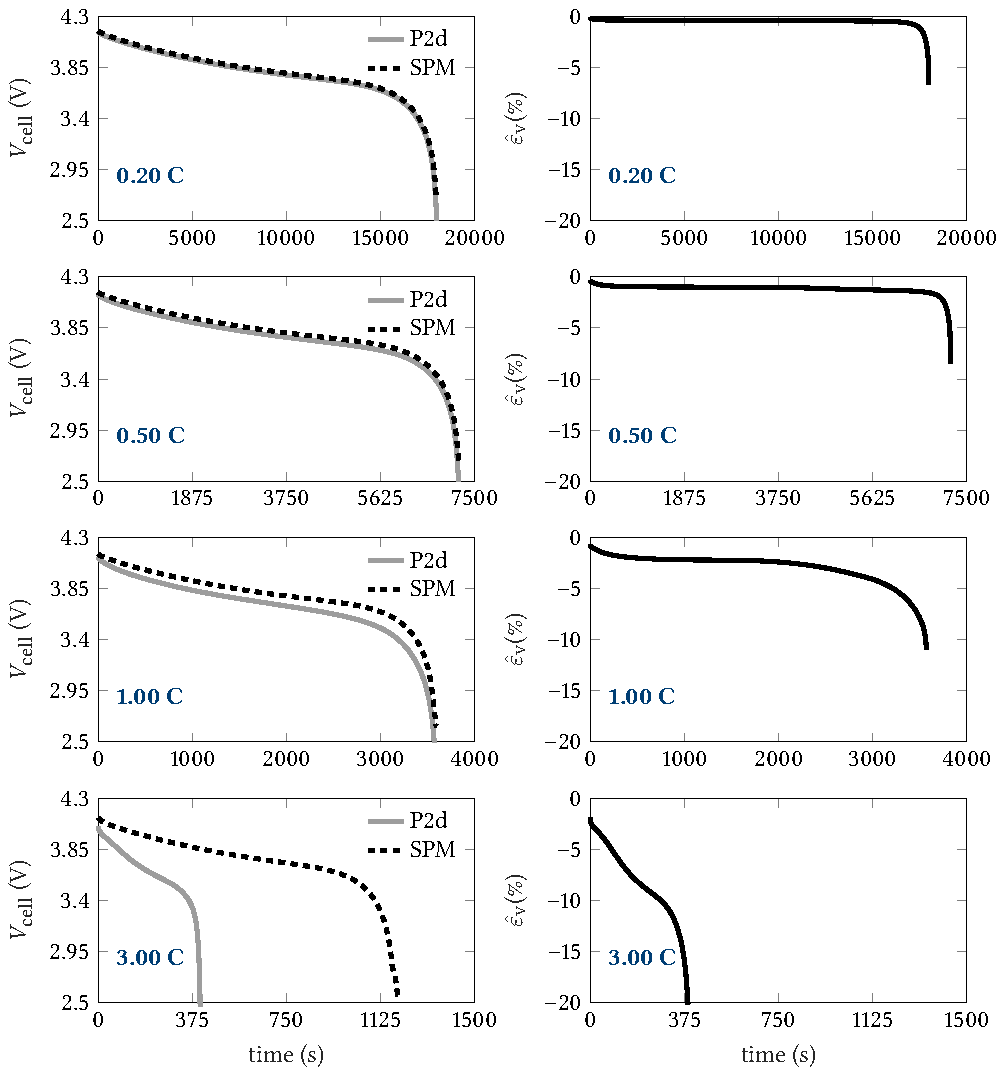
\includegraphics[width=\textwidth]{4/figures/const_curr_dischg_voltage.pdf}
    \caption[Voltage responses of \glsfmtshort{p2d} and \glsfmtshort{spm} to
    constant current discharge]{Voltage responses of the \glsfmtshort{p2d} and
        \glsfmtshort{spm} models to various constant discharge rates. The left
        column column shows the time-domain voltage response of the \gls{spm}
        plotted against the benchmark \gls{p2d} response. The column on the
        right shows the percentage voltage error of the \glsfmtshort{spm} with
        respect to the \glsfmtshort{p2d} model. The performance of the
        \glsfmtshort{spm} degrades considerably at discharge currents above
    0.5C.}
    \label{fig:cnstdischgspmp2dvoltage}
\end{figure}

The  left  column  of~\cref{fig:cnstdischgspmp2dvoltage} shows  the  time-domain
voltage response of the basic \gls{spm} for various constant discharge currents.
The voltage response of the \gls{p2d} model  is also overlaid on these plots and
is used  as a  reference benchmark  for comparisons.  It is  difficult to  use a
common  time-scale for  the horizontal  axes of  the plots  since the  run-times
differ by two orders of magnitude for the C-rates considered.

Since  these comparisons have
to  be done  across  multiple  C-rates, each  yielding  different magnitudes  in
voltage responses,  it is  helpful to use  a relative error  metric such  as the
percentage error, defined as
\begin{equation}
    \hat{\varepsilon}_v\,(\si{\percent}) = 100\frac{V_{\text{cell}_\text{p2d}} - V_{\text{cell}_\text{spm}}}{V_{\text{cell}_\text{p2d}}}
\end{equation}

It is to be noted that, in all cases, the \gls{p2d} model terminates faster than
the \gls{spm} either due to hitting lower cut-offs of either terminal voltage or
\gls{soc} (see~\cref{fig:cnstdischgspmp2dsoc}).  Consequently, the  error vector
is defined only the common time-region before cut-off.

In~\cref{fig:cnstdischgspmp2dvoltage},  the  column  on   the  right  shows  the
percentage error  in the voltage response  of the \gls{spm} with  respect to the
\gls{p2d} model.  At very  low C-rates  below \approx0.5C,  the voltage-response
performance of the \gls{spm} is acceptable. However, the performance degradation
is rapid above this C-rate. It is clear that the error in the \gls{spm} response
is monotonic and unidirectional. This indicates  that the source of the error is
due  to  unmodelled dynamics.  In  particular,  as  discussed in  the  modelling
assumptions  of~\cref{subsec:basicspmassumptions},  the  \gls{spm}  ignores  the
electrolyte dynamics.  Thus, the  overpotential (internal  voltage drop)  in the
electrolyte  is not  modelled,  which results  in the  terminal  voltage of  the
\gls{spm} being always higher than its \gls{p2d} counterpart.

\begin{figure}[!htb]
    \centering
    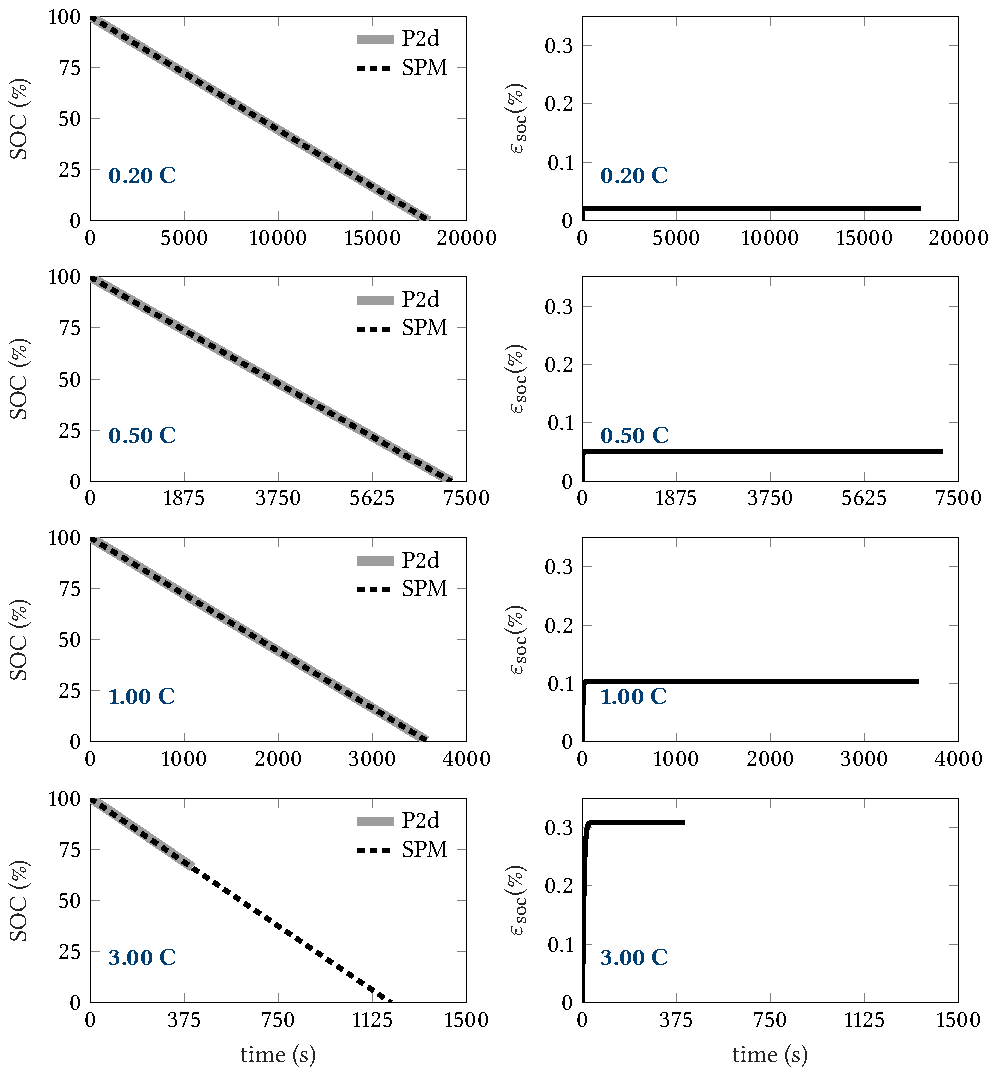
\includegraphics[width=\textwidth]{4/figures/const_curr_dischg_soc.pdf}
    \caption[\glsfmtshort{soc} computed by \glsfmtshort{p2d} and
    \glsfmtshort{spm} models for constant current discharge]{Plots in the left
        column depict the time evolution of \glsfmtshort{soc} computed by the
        \glsfmtshort{p2d} and \glsfmtshort{spm} models for various constant
        discharge rates. The column on the right shows the error of the
        \glsfmtshort{soc} computed by the \glsfmtshort{spm} with respect to that
        computed by the \glsfmtshort{p2d} model, \ie{} $ \varepsilon_\text{soc}
        = {z_\text{p2d}} - z_\text{spm} $. The \glsfmtshort{spm} remains quite
    accurate even at moderate currents such as 3C.}
    \label{fig:cnstdischgspmp2dsoc}
\end{figure}

\Cref{fig:cnstdischgspmp2dsoc}  shows  the  time-evolution  of~\glsfmtshort{soc}
computed by the  \glsfmtshort{p2d} and the \glsfmtshort{spm}  models for various
discharge  currents. Since  the  \gls{soc} of  a cell  is  already a  normalised
quantity by  definition, the difference between  the two models can  be directly
used for comparison across C-rates. The \gls{soc} error is defined as
\begin{equation}
    \varepsilon_\text{soc} = {z_\text{p2d}} - z_\text{spm}
\end{equation}
and like the  error in the  terminal voltage, remains unidirectional  over time,
and defined only until one of the models hits cut-off.

After  perusing the  \gls{spm}'s poor  performance demonstrated  in its  voltage
response,  it  may   be  surprising  to  note  that   its  \gls{soc}  prediction
capabilities remain quite accurate even  at moderate discharge currents of about
3C and warrants a brief explanation.

Referring to~\cref{eq:soccomputation}, it is  seen that the \glsfmtshort{soc} of
the cell  is directly proportional  to the  bulk (average) concentration  in the
negative  electrode.  Hence  the  plots  of~\cref{fig:cnstdischgspmp2dsoc}  also
represent the solid  phase concentration with a constant scaling  factor. As per
the assumptions listed  in~\cref{subsec:basicspmassumptions}, the only transport
phenomena  modelled in  the \gls{spm}  is  solid phase  diffusion. However,  for
computation of the terminal  voltage, the electrolyte overpotential contribution
has  been   omitted  (see~\cref{eq:posoverpotential,eq:negoverpotential}).  This
explains  why  the  voltage  accuracy  suffers  while  the  open-loop  \gls{soc}
computation  remains  accurate.  The  high accuracy  of  \gls{soc}  (and  hence,
solid-phase  concentration)   computation  also  validates  the   usage  of  the
\engordnumber{4}  order  polynomial  approximation  instead of  Fick's  law  for
modelling solid-phase diffusion.

However,  the  discrepancy  in  accuracies of  terminal  voltage  and  \gls{soc}
computed  by the  basic \gls{spm}  leads to  an important  implication. Even  at
moderate C-rates, the  basic \gls{spm} \emph{cannot} be effectively  used in the
design of \gls{soc}  observers. This is because, the measured  voltage maps to a
vastly different  operating point when using  the \gls{spm} as the  plant model,
leading to strong deviations of the estimated \gls{soc}.

\subsubsection*{Constant current charge}\label{subsubsec:cnstcurrchgsim}

The \gls{cccv} charging  profile is a widely adopted  standard charging strategy
for charging lithium  ion cells. In the constant current  phase, a charging rate
of 1C is  used as an accepted baseline, although  faster charging strategies are
being actively sought  after both in academia and in  particular, the automotive
industry. For establishing the charging performance of the basic \gls{spm}, the
standard rate of 1C is used.

\begin{figure}[!htb]
    \centering
    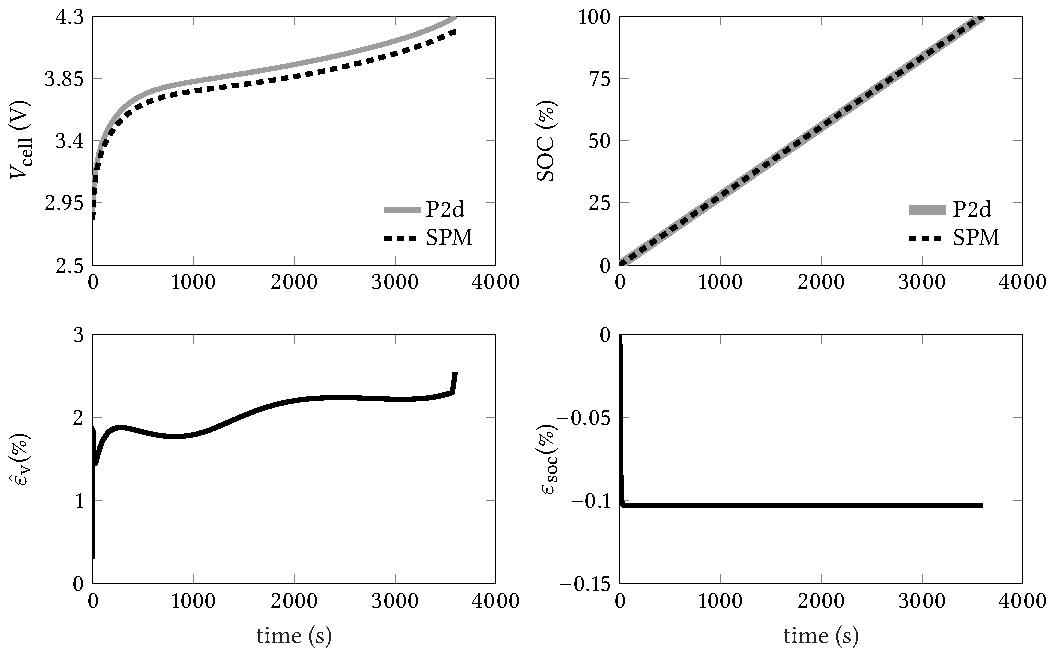
\includegraphics[width=\textwidth]{4/figures/const_curr_chg.pdf}
    \caption[Voltage and \glsfmtshort{soc} evolution of \glsfmtshort{p2d} and
    \glsfmtshort{spm} for 1C constant current charging]{Time evolution of
        voltage and \glsfmtshort{soc} (top row) of the \glsfmtshort{p2d} and
        \glsfmtshort{spm} models upon charging with a constant current of 1C,
        \ie{} \SI{60}{\ampere} starting at \SI{0}{\percent} \glsfmtshort{soc}.
        The bottom row shows the percentage in terminal voltage and
        \glsfmtshort{soc} respectively of the \glsfmtshort{spm} with respect to
    the \glsfmtshort{p2d} model.}
    \label{fig:cnstchgspmp2d}
\end{figure}

The top row of~\cref{fig:cnstchgspmp2d} shows  the evolution of terminal voltage
and \gls{soc}  of the \gls{p2d} and  \gls{spm} models under an  applied charging
current of  1C, \ie{} \SI{60}{\ampere}.  The constant-voltage charging  phase is
not shown. The bottom row shows  the corresponding errors of the \gls{spm} model
with respect  to the reference  \gls{p2d} benchmark. The corollary  behaviour of
the constant current discharge behaviour  is observed here. The terminal voltage
of the \gls{spm} remains below the  \gls{p2d} model throughout. This is expected
since, to  account for the electrolyte  voltage drop in the  \gls{p2d}, a higher
terminal voltage needs  to be applied. The voltage error  is thus unidirectional
and remains positive (opposite to  that observed for the corresponding discharge
case).  Similarly,  the \gls{soc}  plots  overlap  very closely  validating  the
underlying polynomial approximation of solid  phase diffusion. It is striking to
note  that the  error in  \gls{soc} remains  exactly around  the same  magnitude
(\approx\SI{0.1}{\percent}) in both the charging and discharging cases.

The high accuracy of the \gls{soc} in  the basic \gls{spm} leads to the author's
hypothesis that if the electrolyte concentration can be solved as an independent
subsystem and  incorporated into the  terminal voltage, this  can lead to  an improved
\gls{spm}  with electrolyte  dynamics. Such  a decoupled  electrolyte inclusion
into the basic \gls{spm}\fxnote{fix this sentence}

% textwidth in cm: \printinunitsof{cm}\prntlen{\textwidth} % 15.74776 cm
% textwidth in cm: \printinunitsof{cm}\prntlen{\textheight} % 22.27184 cm
% electrolyte resistance
% github toolbox

% % -*- root: ../main.tex -*-
%!TEX root = ../main.tex
% this file is called up by main.tex
% content in this file will be fed into the main document
% vim:textwidth=80 fo=cqt

As  evidenced by  the  results of  the constant  current  charge, discharge  and
dynamic  simulation runs,  the basic  \gls{spm} suffers  from a  \emph{critical}
drawback. The lack of electrolyte dynamics in the conventional \gls{spm} results
in poor  voltage accuracy  even at  moderate {C-rates}.  This renders  the model
unsuitable for  observer design in  \gls{soc} estimation applications  since the
output voltage from the model maps  to a radically different \gls{soc} operating
point. A number of candidate solutions have been proposed in literature in order
to mitigate this drawback. Their salient aspects are briefly evaluated here.

Even  the earliest  works which  attempt  to include  electrolyte dynamics  into
the  conventional  \gls{spm} were  published  only  within the  present  decade.
Schmidt~\etal~\cite{Schmidt2010c} proposed  an infinite-sum  eigenfunction modal
expansion paradigm for solving for the electrolyte concentration. It was claimed
that by  accounting for contribution from  only the first two  terms, sufficient
accuracy may be achieved. Furthermore, an \gls{ode} was proposed for the rate of
evolution of  the first temporal  mode. The solved electrolyte  concentration is
then  substituted into  an  approximate analytical  solution  for the  \gls{dfn}
model's  charge conservation  \gls{pde}\fxnote{cross-reference  to Newman  model
equation here}  to obtain the  electrolyte potential. However,  the presentation
lacks the  sufficient depth  of explanation  which hinders  reproducibility. For
instance,  the  origin  and  explanation  of  the  approximation  terms  in  the
electrolyte  potential solution  is omitted.  Derivations are  performed from  a
rigorous mathematical perspective without providing contextual reference to cell
parameters or  electrochemical quantities. Introducing numerical  examples would
have been a redeeming factor to help keeping the mathematical aspects tractable.
This method has not seen further uptake for \gls{spm} modelling.

Guo~\etal~\cite{Guo2011a}  presented an  empirical approach  to account  for the
solution-phase dynamics.  Using standard curve-fitting techniques,  a non-linear
resistance as  a function of current  and temperature was introduced.  Thus, the
equation for cell terminal voltage presented
in~\cref{eq:cellterminalvoltagebasic} is modified as
\begin{equation}
    V_\text{cell} = η_\text{pos} - η_\text{neg} + U_\text{pos} - U_\text{neg} - I R_\text{eq}
\end{equation}
where  $R_\text{eq}$  is the  equivalent  resistance  newly introduced.  In  the
opinion of  this thesis  author, this  approach is too  simplistic and  does not
generalise well. Even if giving up  physics-based model origins can be tolerated
for one  or two subsystems  within the model,  the equivalent resistance  is not
just a minor correction term since it  needs to account for a large polarization
voltage of  the order  of tens of  millivolts. Secondly,  the current-dependence
introduced  to account  for the  complex mass  and charge  transport within  the
electrolyte  places a  disproportionately large  weight on  the accuracy  of the
curve-fitting process. Non-linear fits as proposed in Guo~\etal{} are inherently
problematic  in nature  as  the optimisation  routine may  converge  to a  local
minimum.  The specific  form and  nature, \eg{}  the convexity  of the  proposed
hypothesis function is  not discussed. Also, it is also  not guaranteed that the
same fitting  function is  applicable to  a different cell  with another  set of
parameters. Finally,  the correction  term being resistive  in nature  is zeroth
order,  \ie{}  cannot account  for  the  frequency  dependent behaviour  of  the
electrolyte's  dynamics. This  approach is  more suited  for small-scale  static
corrections that do not depend on the current,\eg{} to account for a few tens of
microvolts  due to  a constant  contact  resistance of  the current  collectors.
\fxnote{later on, as a capstone work, mention how I was inspired}

Di   Domenico~\etal{}~\cite{DiDomenico2010}  were   the  first   to  present   a
step-by-step  derivation   of  the   approximate  analytical  solution   to  the
electrolyte overpotential. The potential drop in the electrolyte is given by
\begin{equation}\label{eq:electrolytepd}
    \phi_\epos - \phi_\eneg = -\frac{I}{2 A}\left(\frac{l_\text{neg}}{\kappa_\text{eff}} + 2 \frac{l_\text{sep}}{\kappa_\text{eff}} + \frac{l_\text{pos}}{\kappa_\text{eff}}\right)
\end{equation}
and     can     be     substituted    into     the     subtraction     operation
involving~\cref{eq:posoverpotential} and~\cref{eq:negoverpotential} in computing
the   overall  overpotential   of~\cref{eq:overpotentialdifference}  and   hence
the  terminal  voltage.  The  effective   conductivity  of  the  electrolyte  in
a   given   region   \jinpossepneg{},   within   the   cell,   is   defined   as
$\kappa_\effj(c_e) = \kappa(c_e)\, \varepsilon_j^{\text{brugg}_j}$. As discussed
in~\cref{subsec:basicspmsimsetup},  the   intrinsic  and  hence   the  effective
electrolyte conductivity is a function of the concentration of \ch{Li^+} ions in
the  electrolyte.  Di  Domenico~\etal{}  did  not  discuss  the  spatio-temporal
calculation  of  electrolyte  concentration.  It   is  likely  that  a  constant
electrolyte concentration  at its  initial equilibrium value  was used.  As seen
in~\cref{fig:ce1cdischgwithzoom}\fxnote{do not  forget to  show the  gradient in
$c_e$}, significant spatial gradients in the electrolyte are established at even
low to moderate {C-rates} during  the cell's operation. Sustained application of
a unidirectional  current even leads to  starvation of ions in  the electrolyte,
particularly  near  the  current   collectors.  This  phenomenon  is  visualised
in~\cref{fig:ce1cdischgwithzoom} wherein the electrolyte at the positive current
collector  is  virtually  depleted  of  ions  at  the  end  of  discharge.  This
ion-starvation process occurs earlier at higher {C-rates} and spreads throughout
the  thickness  of  the  electrode.  Thus,  the  assumption  of  constant  ionic
concentration  in the  electrolyte is  not true.  Neglecting mass  transport due
to  diffusion  implies  that  the  terms  in~\cref{eq:electrolytepd}  constitute
only  a part  of the  expression  for computing  the electrolyte  overpotential.
Furthermore, Di Domenico~\etal{} do not  present any results of applying dynamic
current profiles.  Since the critical  aspect of mass transport  contribution to
electrolyte  overpotential  is  omitted,  this  model  cannot  be  viewed  as  a
\emph{sufficient} enhancement to the basic \gls{spm}.

\begin{figure}[!htp]
    \centering
    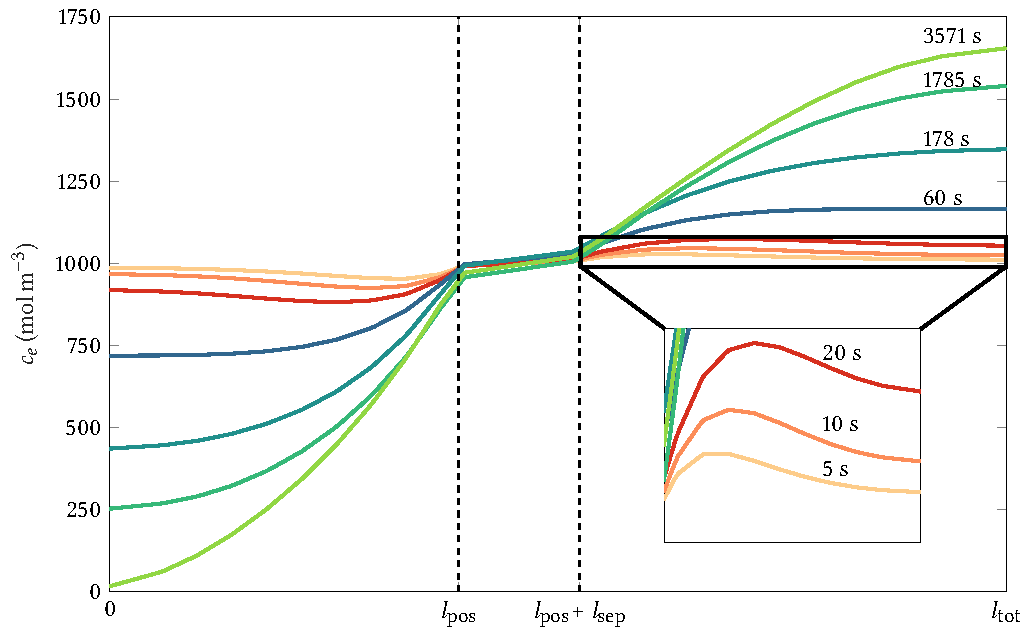
\includegraphics{4/figures/ce_1C_at_various_times.pdf}
    \caption[Electrolyte conc.\ (time-snapshots) along cell thickness for 1C
    discharge]{\ch{Li^+} ion concentration in electrolyte along cell thickness
        at various time-snapshots during a 1C discharge simulation of the
        \glsfmtshort{p2d} model. A \glsfmtlong{qss} (\glsfmtshort{qss}) spatial
        profile  with inflection point at each separator interface begins to
        form at \approx \SI{60}{\second} after discharge begins. However, the
        ionic concentration in electrolyte exhibits a significantly different
        transient behaviour (zoomed inset) possessing another inflection point
        that disrupts the monotonic trend. Depletion of ionic concentration at
        positive current collector  towards end of discharge is also seen
    (bottom left).}
    \label{fig:ce1cdischgwithzoom}
\end{figure}

Although  not presented  in the  context  of incorporating  into the  \gls{spm},
Guduru~\etal~\cite{Guduru2012}   derived   an   analytical   solution   of   the
spatio-temporal  evolution  of  electrolyte concentration  using  the  \gls{sov}
method. The \gls{sov} method was first  applied to lithium ion cell modelling by
Subramanian~\etal~\cite{Subramanian2001a}  in order  to  solve  for solid  phase
concentration  profiles in  spherical  electrode particles.  Although the  ionic
concentration  in  the electrolyte  computed  by  the analytical  expression  in
Guduru~\etal{} seems like a feasible choice for inclusion into the \gls{spm}, it
is only applicable for galvanostatic boundary conditions, \ie{} when the applied
current  is held  constant over  time. By  natural extension,  researchers could
hypothesise  that this  restriction  may  be removed  by  considering the  input
current as  piecewise constant  over small sample  intervals. Such  a hypothesis
could  be  reinforced  by  the  fact that  standard  drivecycles  are  specified
as  discrete  samples and  the  discrete-time  \gls{spm} processes  these  input
samples assuming \gls{zoh} behaviour. However, the analytical solution presented
in  Guduru~\etal{}  assumes  a  \gls{qss} concentration  profile.  The  authors'
presentation  considers a  near-instantaneous  establishment  of this  \gls{qss}
and  suggests a  parameter  independent analysis  through  use of  dimensionless
concentrations and time-constants instead of absolute time.

In  the  studies  conducted  by  this  thesis  author,  significantly  different
transient  behaviour  is exhibited  by  the  electrolyte concentration  profile.
Furthermore,  the  time  taken  to   establish  the  \gls{qss}  profile  is  not
negligible. This  difference in behaviour  could be attributed to  the different
parameter  set used.  \Cref{fig:ce1cdischgwithzoom}  shows  the spatial  profile
of  ionic concentration  at  various  snapshots of  time  during  a 1C  constant
current discharge. Starting at \SI{100}{\percent} \gls{soc}, the discharge lasts
\SI{3571}{\sec}. It is  seen that it takes nearly  \SI{60}{\second} to establish
the  approximately parabolic  shape  assumed by  the electrolyte  concentration.
After  the  initial transient  has  elapsed,  the  underlying structure  of  the
mathematical equations  can be assumed  to be static.  This is evidenced  by the
fact that at \SI{1785}{\second}, \ie{} after half of the discharge is completed,
the shape of the curve is nearly  identical to the one towards end of discharge.
These  \gls{qss} curves  have their  sole inflection  points at  their separator
interfaces and remains monotonic within  their respective electrode regions. The
difference in  height for  various times  can be  accounted by  the coefficients
solved using the analytical modal solution proposed in Guduru~\etal{}.

The  axes  in  the  inset  of~\cref{fig:ce1cdischgwithzoom}  shows  a  zoomed-in
view  of  the electrolyte  concentration  during  the transient  phase,  wherein
the  \gls{qss}  has  not  yet  been  established.  In  particular,  there  exist
additional inflection points,  one within the interior of  each electrode, which
renders the transient concentration profile mathematically incompatible with the
monotonicity  exhibited  by  the  \gls{qss} profile.  Thus,  in  highly  dynamic
operating  conditions with  frequent reversals  in  the direct  of current,  the
\gls{qss} assumption for the galvanostatic analytical solution becomes harder to
uphold without introducing significant  errors. Finally, the analytical solution
profile in Guduru~\etal{}  is not amenable to embedded  implementation, since it
consists of a non-trivial set of trigonometric computations at each time-step.

Prada~\etal~\cite{Prada2012} were  the first to provide  a simplified expression
for potential drop in the electrolyte  by including the terms representing ionic
concentration gradient within the cell thickness. Thus, \cref{eq:electrolytepd}
gets modified as
\begin{equation}\label{eq:electrolytepdwithce}
    \phi_\epos - \phi_\eneg = (1-t_{+}^0) \frac{2RT}{F}\ln
    \frac{c_\text{e,\tiny pos/cc}}{c_\text{e,\tiny neg/cc}}-\frac{I}{2 A}\left(\frac{l_\text{neg}}{\kappa_\text{eff}} + 2 \frac{l_\text{sep}}{\kappa_\text{eff}} + \frac{l_\text{pos}}{\kappa_\text{eff}}\right)
\end{equation}
Although  the complete  expression for  electrolyte overpotential  was provided,
it   was  presented   in  a   cursory  manner,   \ie{}  without   detailing  the
spatio-temporal  computation  of  ionic  concentration  values  at  the  current
collector interfaces.  Nevertheless, it is  important to note  this contribution
as~\cref{eq:electrolytepdwithce} is widely relied  upon by subsequent literature
and shall be used in the original work of electrolyte concentration distribution
presented by this thesis author in~\cref{sec:newelectrolytemodel}.


Rahimian~\etal{}~\cite{KhaleghiRahimian2013}   were   the   first   to   provide
approximate expressions for both charge  transport and mass transport properties
of the electrolyte specifically with the focus on improving the basic \gls{spm}.
The  authors discuss  the usage  of a  polynomial approximation  for electrolyte
concentration and potentials.  In particular, a cubic polynomial  was chosen for
approximating the  electrolyte concentration within the  porous electrodes. This
necessitates the  need to solve  for eight coefficients for  uniquely describing
the electrolyte concentration profile within  the electrode regions. However, in
the standard \gls{dfn} model, the number of electrolyte-specific \glspl{pde} and
their corresponding boundary conditions describing  charge and mass transport is
insufficient to uniquely  solve for all unknown coefficients  of this polynomial
approximation.  A detailed  explanation  of this  equation  deficiency shall  be
discussed in~\cref{temp:eqndeficiency}.

To overcome the issue of  equation deficiency, Rahimian~\etal{} adopted a scheme
wherein one  additional spatial location in  the interior of each  electrode was
also needed. The coefficients of the polynomial approximation were then obtained
by iteratively solving a large  coupled system of algebraic equations, embedding
within  them  the additional  equations  evaluated  at  the interior  points.  A
complicating issue  that arises  is regarding the  optimal positioning  of these
additional interior  points. An online  numerical optimisation was  performed to
obtain  the optimal  placement of  this interior  node. In  the opinion  of this
thesis author, these optimisation results could be sensitive to the thickness of
the electrodes  among other  parameters. A  discussion of  the stability  of the
proposed routine and its robustness to  parameter variance shall help in lending
confidence in the proposed method.  Although sufficient accuracy of the improved
\gls{spm} was  demonstrated for  currents up  to 5C, a  notable omission  is the
discussion of the model's performance  to dynamic input profiles. In conclusion,
the author of this thesis opines that, although this method serves as a proof of
concept towards implementing polynomial approximations for electrolyte dynamics,
until the aforementioned  gaps are addressed with clarity, it  is not convincing
for uptake by relevant stakeholders.

Kemper  and  Kum~\cite{Kemper2013} presented  an  approach  wherein the  spatial
gradients of the electrolyte concentration  are neglected. The time-evolution of
\emph{average}  ionic concentration  in each  of the  three cell  regions \viz{}
positive electrode, separator  and negative electrode are described by  a set of
three \glspl{ode}. As established by  the discussion thus far, the concentration
gradients along the axial thickness of the cell is significant, even at moderate
{C-rates}. Lending strength to doubts on  the model's wider applicability is the
fact that results from constant current inputs (which induce large concentration
gradients  in electrolyte)  have  not been  reported in  this  work. Thus,  this
approach is deemed as not satisfactory enough to warrant further engagement.

Luo~\etal~\cite{Luo2013} derived  a parabolic  approximation of  the electrolyte
concentration  distribution along  the  thickness of  the  cell. The  derivation
is  obtained  for  the case  of  steady-state  wherein  the  rate of  change  of
concentration  is  zero.  However,  the  author  of  this  thesis  is  sceptical
about  this   since  in  the   simulations  performed  there  is   no  situation
other  than  prior  to  application  of current  that  this  exact  steady-state
condition is  satisfied. In  the \gls{qss} profile  concept discussion  based on
on~\cref{fig:ce1cdischgwithzoom},  it  is  clear that  only  the  \emph{spatial}
profile reaches  a shape that can  be potentially described by  a mathematically
invariant   family   of  curves.   The   electrolyte   concentration  is   still
\emph{time-varying} and therefore violates the static time-evolution assumption.
Although  Luo~\etal{}  do  not  explicitly acknowledge  this,  they  provide  an
extension for  general operating  conditions by introducing  exponential scaling
functions  $f_n(t)$ and  $f_p(t)$ while  retaining the  assumption of  parabolic
spatial behaviour.  The computation of  certain time-constants in  these scaling
functions  are  not  elucidated  nor  is  a  summary  of  procedural  steps  for
determination of the aforementioned scaling functions provided.


In a subsequent paper by  the same authors, \ie{} Luo~\etal~\cite{Luo2013a}, the
electrolyte concentration  model together  with a  similarly-derived electrolyte
potential model  was incorporated into  the conventional \gls{spm} to  arrive at
what the authors term as extended \gls{spm}. In this work, the electrolyte
potential is set to account for contribution from two terms ---
\begin{enumerate*}[label=\emph{\alph*})]
    \item ohmic drop due to bulk solution resistance and
    \item polarization potential due to concentration gradients
\end{enumerate*}
Although it  seeks to correctly account  for the two causes  of overpotential in
the  electrolyte,  there  is  no  detailed explanation  on  the  computation  of
quantities such as time-constants involved in the polarization potential term.

A modified version of the electrolyte model proposed in Luo~\etal~\cite{Luo2013}
was  used in  Zhou~\etal~\cite{Zou2016a}  for observer  design  in an  \gls{soc}
estimation application. The modification  essentially consists of truncating the
complex  expression  in~\cite{Luo2013}  consisting of  six  coefficients,  $p_1$
through $p_6$ to just two, and elimination of the aforementioned time-constants.
However, to  the disappointment  of the  author of this  thesis, the  claim that
truncation to  $n=2$ terms is sufficient  to describe the dynamics  proved to be
optimistic for  the parameter set considered.  In my attempts to  reproduce this
work, an  arbitrary scaling  factor was  needed to  correct for  the electrolyte
potential drop  and match  the \gls{p2d} simulations.  The requirement  for such
scaling factors  whose physical  origins are not  clearly identifiable  lends to
scepticism on the model's robustness. Furthermore,  it was found that this value
needed to be  hand-tuned for each parameter-set. Until these  gaps are addressed
clearly, it is worth seeking other  viable alternatives to model the electrolyte
dynamics.

After  completing  the  simulations  with  the  aforementioned  scaling  factors
and  continuing  in  the  quest  for other  alternatives,  the  author  of  this
thesis  made  an observation  that  other  researchers  have  had to  resort  to
similar techniques  for describing the electrolyte  overpotential. For instance,
Han~\etal~\cite{Han2015a}  use   a  similar   scaling  factor,  $p<0$   for  the
entire expression of~\cref{eq:electrolytepdwithce}  representing the electrolyte
overpotential.  In this  case,  these authors  used  a polynomial  approximation
approach proposed in  Rahimian~\etal~\cite{KhaleghiRahimian2013}. However, these
unexplained scaling factors lower the level of confidence in the model's general
applicability.


Tanim~\etal~\cite{Tanim2014}  accounted  for  electrolyte dynamics  by  deriving
reduced   order  transfer   functions  for   ionic  concentration   distribution
and   electrolyte  overpotential   using  the   \gls{ima}  technique.   However,
the  coefficients  of   these  transfer  functions  are   excessively  long  and
comprised  of   chained  algebraic   operations  expressed  in   a  high-entropy
sum-of-products  form  in  the  appendix   of  their  work.  For  instance,  ten
coefficients  are  needed  to  describe  the  concentration  profile  while  six
coefficients  are required  for  the electrolyte  potential.  The median  length
of  each  atomic  sub-expression  of these  coefficients  is  sufficiently  high
to  obfuscate   their  physical  significance.   A  low-entropy  form   for  the
coefficients  of  these   transfer  functions  similar  to   that  pioneered  by
Middlebrook~\cite{Middlebrook} and  exemplified in the  design-oriented analysis
of  electric   circuits~\cite{Middlebrook1998,Vorperian2002}  could   have  been
helpful to aid the readers' understanding.  The author of this thesis recognises
that  mathematical complexity  should  not be  the sole  basis  to evaluate  the
merits of  such proposed improvements.  Although the presentation of  these long
coefficients have been judiciously moved  to the appendix, their derivations ---
essential to prove the model's validity  --- is curiously omitted. The length of
the mathematical  expressions increases  the probabilities of  introducing human
errors during implementation.

It  is worth  noting that  Marcicki~\etal~\cite{Marcicki2013} had  independently
proposed a similar approach, \viz{}  deriving a transcendental transfer function
from  electrolyte  concentration  to  applied  current, albeit  for  a  cell  of
\gls{lfp} chemistry. This transfer function  consisted of a series of hyperbolic
trigonometric functions which  were later truncated by  Padé approximation (see
\cref{subsec:freqdomainroms}  for  a  brief  introduction  to  frequency  domain
\glspl{rom}). However, upon trying this approach for the \gls{lco} parameter set
by this thesis'  author, in order to obtain sufficient  accuracy, the truncation
order had  to be  raised to  at least seven,  similar in  complexity to  that of
Tanim~\etal~\cite{Tanim2014a}.  In  both Marcicki~\etal~\cite{Marcicki2013}  and
Tanim~\etal~\cite{Tanim2014a},  the  electrolyte-specific  enhancements  to  the
\gls{spm} are in  the frequency domain, placing further  burden, particularly on
industry stakeholders to accurately interpret  and transform the coefficients to
a time-domain implementation  for deployment in an embedded  \gls{bms}. Owing to
this,  as  already  stated in~\cref{subsec:freqdomainroms},  these  models  fall
outside the scope of this thesis.
% ignoring prof plett's latest work on electrolyte transfer functions

Fan~\etal~\cite{Fan2016}   proposed   an   Extended  \gls{spm}   that   includes
electrolyte dynamics using  the \gls{gpm} which achieves  an acceptable accuracy
in terminal voltage  performance. Although the authors claim  that the \gls{spm}
is computationally  \emph{cheaper} than  other model order  reduction techniques
such as proper orthogonal decomposition  and balanced truncation, this claim has
not  been substantiated.  The sole  comparison of  CPU times  presented in  this
work  only compares  against  the classical  \gls{fdm}.  Although an  impressive
computational  speed is  achieved, it  is  unclear whether  the model  equations
particularly  those  involving  solutions  of  non-linear  integral  expressions
resulting from  applying the Galerkin's  method can  be solved in  real-time for
embedded implementation.  In the review of  this method conducted by  the author
of  this thesis,  it  appears  that the  Galerkin's  projection  method is  more
suitable  for  desktop  simulations.  In  congruence  with  my  scepticism,  the
authors  of~\cite{Fan2016} have  not claimed  the suitability  of this  work for
online/embedded  application  in a  \gls{bms}.  Therefore,  as per  this  thesis
authors' stance  explained in~\cref{sec:classificationscheme},  models employing
such methods are deemed to be not in alignment with the goals of this thesis.

Moura~\etal~\cite{Moura2017} propose an improved  \gls{spm} by simply augmenting
the  conventional  \gls{spm}  with  a simplified  form  of  electrolyte-specific
equations of  the original  \gls{dfn} model. The  resulting model  therefore has
\glspl{pde} in it and therefore not easily amenable for embedded implementation.
The other main  contribution of this work is its  feasibility analysis of having
convergent  estimators for  this  model  and design  of  such a  \gls{pde}-based
estimator.  In  the  views  of  this  thesis  author,  this  approach  is  on  a
trajectory that  deviates too far  from a  simplified model suitable  for online
implementation.

Lofti~\etal~\cite{Lotfi2017}  presented  an   algebraic  approximation  for  the
spatial  distribution   of  electrolyte  concentration  by   modifying  standard
parabolic expressions with leading exponential  coefficients. There are two main
issues with this approach. It is not explained why this mathematical formulation
was chosen  and its superiority  with respect to other  family of curves  is not
discussed. Secondly, these coefficients are to be determined through solution of
equations obtained by applying continuity  and flux boundary conditions from the
\gls{dfn}  model  for  electrolyte  concentrations  at  the  electrode-separator
interfaces. Since exponential-type expressions are assumed, the resulting set of
equations  are  non-linear, whose  solution,  especially  in  the context  of  a
resource-constrained environment is problematic.

In  the authors'  observations, the  errors  in these  model approximations  can
be  attributed  to  inaccuracies  in  computing  the  spatio-temporal  evolution
of  electrolyte   concentration.  Upon   obtaining  a   good  estimate   of  the
electrolyte concentration profile,~\cref{eq:electrolytepdwithce} is deemed to be
satisfactory for  the electrolyte  overpotential computation. Thus  attention is
focussed on solving for the electrolyte concentration profile.

From the discussion of literature, it is clear that the proposed enhancements to
the  computing the  ionic concentration  in electrolyte  falls into  one of  the
following two categories:
\begin{itemize}
    \item model description through physical principles followed by mathematical
        simplification
    \item fitting of pre-assumed simplified mathematical structures to some
        physical phenomena
\end{itemize}

In the  views of the  author, it appears that  using the former  approach yields
technically  correct, yet  mathematically convoluted  expressions overpotentials
that are fraught with implementation  difficulties. Although the latter approach
looks  promising  in   terms  of  ease  of   implementation,  their  sub-optimal
performance and lack of wider-applicability leaves much to be desired. Among the
latter  class of  models,  the quadratic  (parabolic)  approximation method  for
electrolyte concentration  is the most widely  used\fxnote{citations needed}. It
is therefore  important to understand  the source  of weakness of  this specific
sub-class  of  models  which  have  not been  discussed  in  literature.  Hence,
the  author's analysis  on the  quadratic approximation  method for  electrolyte
concentration is presented next in~\cref{sec:quadraticapprox}.


% May also mention some typographical errors in Lofti etal second paper
% Mention that parabolic profile is a common theme
% perhaps it cannot be done, but we do not give up. Equation deficiency

% But I  did something different. The high accuracy  of the \gls{soc}
% in  the  basic  \gls{spm}  leads  to  the  author's  hypothesis  that  if  the
% electrolyte  concentration  can be  solved  as  an independent  subsystem  and
% incorporated into the terminal voltage, this can lead to an improved \gls{spm}
% with electrolyte  dynamics. Such  a decoupled  electrolyte inclusion  into the
% basic \gls{spm}\fxnote{fix this sentence}


% % -*- root: ../main.tex -*-
%!TEX root = ../main.tex
% this file is called up by main.tex
% content in this file will be fed into the main document
% vim:textwidth=80 fo=cqt

In   this    section,   the    quadratic   approximation   of    ionic   spatial
concentration,   that  underpins   the  electrolyte   model  in   many  improved
\gls{spm}  formulations  is  presented.  The  steps  involved  in  deriving  the
quadratic   approximation   is  detailed   in~\cref{subsec:quadraticmodelderiv}.
In~\cref{subsec:quadraticsimresultsanalysis},  an analysis  of  the weakness  of
this  model is  performed  based  on the  results  from  applying the  quadratic
approximation scheme. Mitigation of this critical drawback lead to this author's
decoupled  spatio-temporal electrolyte  concentration model  structure which  is
presented next in~\cref{sec:newelectrolytemodel}.

\subsection{Model derivation}\label{subsec:quadraticmodelderiv}

\begin{figure}[!htb]
    \captionsetup{singlelinecheck=off}
    \centering
    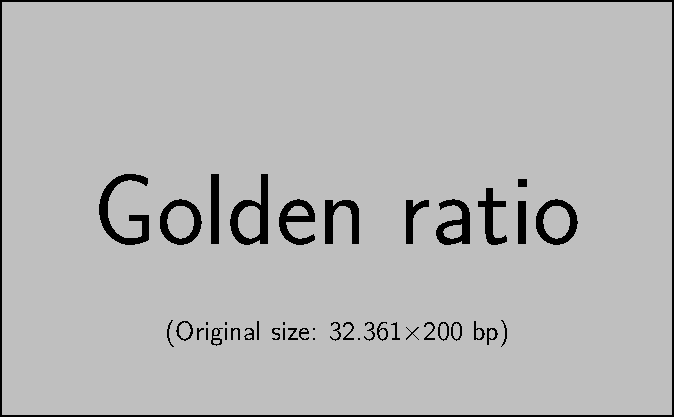
\includegraphics{placeholder_images/example-image-golden.pdf}
    \caption[Co-ordinate systems for quadratic approximation of
    electrolyte concentration]{Schematic diagram of the electrochemical sandwich
        consisting of
        \begin{enumerate*}[label=\itshape\alph*\upshape)]
            \item negative electrode,
            \item separator, and
            \item positive electrode
        \end{enumerate*} depicting the co-ordinate system used in deriving the
        quadratic approximation profile. The global spatial co-ordinate is $x
        \in \{0,l_\text{tot}\}$, where $l_\text{tot} = l_\text{neg} +
        l_\text{sep} + l_\text{pos}$. Local co-ordinate systems specific to each
        region are also defined. It should be noted that the positive
        electrode's local co-ordinate axis direction is reversed.}
    \label{fig:coordsquadapprox}
\end{figure}

The  schematic  in~\cref{fig:coordsquadapprox}  shows   the  definition  of  the
co-ordinate  systems  used  in  deriving the  polynomial  approximation  of  the
electrolyte concentration  profile. The globally defined  $x$ co-ordinate starts
at  the negative  current  collector  interface ($x=0$)  and  terminates at  the
positive  current  collector  interface  ($x =  l_\text{tot},\,  l_\text{tot}  =
l_\text{neg} +  l_\text{sep} +  l_\text{pos}$). Three local  co-ordinate systems
$z_\mu$  valid  only  within  their  respective regions  are  also  defined.  In
particular, it  must be  noted that  the direction  of the  local $z_\text{pos}$
co-ordinate axis is opposite to that of  the other two local co-ordinate axes as
well as the global co-ordinate axis. In subsequent usages, the suffix in $z_\mu$
is dropped and  the reader is advised  to infer the region of  validity from the
usage  context  which are  unambiguous  as  they  occur in  separate  equations.
Furthermore, the  notation of  the three regions  $\{\text{neg, sep,  pos}\}$ is
abbreviated  to $\{n,s,p\}$  respectively in  all mathematical  expressions. The
author  is convinced  that this  notation does  not detract  from following  the
derivations, but rather aids it by keeping the notations compact.

A  standard  quadratic expression  is  chosen  a  priori for  approximating  the
electrolyte concentration profile within each region.
\begin{alignat}{2}
    c_\ensub(z,t) & = a_2(t) z^2 + a_1(t) z + a_0(t) \qquad &  & 0 \le z \le l_\text{n}\label{eq:cenqquadstart}   \\
    c_\essub(z,t) & = a_5(t) z^2 + a_4(t) z + a_3(t) \qquad &  & 0 \le z \le l_\text{s}\label{eq:cesqquadstart}   \\
    c_\epsub(z,t) & = a_8(t) z^2 + a_7(t) z + a_6(t) \qquad &  & 0 \le z \le l_\text{p}\label{eq:cepqquadstart}
    \shortintertext{where     the    coefficient     vector    $\vec{a}(t)     =
    \vect{a_0(t),a_1(t),   \dots  ,a_8(t)}$   is  to   be  determined   at  each
    time-step\footnotemark.  Applying  boundary  conditions of  the  electrolyte
    diffusion equation from  the \gls{dfn} model~(refer~\cref{eq:dfnliquiddiff})
    to~\crefrange{eq:cenqquadstart}{eq:cepqquadstart},  it  is clear  that  $a_1
    =  0$ and  $a_7  = 0$.  Thus,~\crefrange{eq:cenqquadstart}{eq:cepqquadstart}
    become}
    c_\ensub      & = a_2 z^2 + a_0         \qquad          &  & 0 \le z \le l_\text{n}\label{eq:cenquadreduced} \\
    c_\essub      & = a_5 z^2 + a_4 z + a_3 \qquad          &  & 0 \le z \le l_\text{s}\label{eq:cesquadreduced} \\
    c_\epsub      & = a_8 z^2 + a_6         \qquad          &  & 0 \le z \le l_\text{p}\label{eq:cepquadreduced}
\end{alignat}
\footnotetext{In rest of  the equations, time-dependence of  the coefficients is
dropped from  the notation. It is  implicitly noted that they  are time-varying.
Similarly, spatio-temporal dependence of the electrolyte concentration functions
$c_\text{e,j}$ is omitted  in circumstances where such explicit  notation is not
crucial  for  understanding.} with  the  coefficient  vector being  modified  to
$\vec{a} = \vect{a_0,a_2, \dots ,a_6, a_8}$.

% -*- root: ../main.tex -*-
%!TEX root = ../main.tex
% this file is called up by main.tex
% content in this file will be fed into the main document
% vim:nospell textwidth=180 foldlevelstart=3 foldlevel=3 conceallevel=0

\begin{table}[!htb]
    \centering
    \caption[Electrolyte equations \& boundary conditions of \glsfmtshort{dfn} model in separator]{Electrolyte-specific governing equations and boundary conditions of the \glsfmtlong{dfn} model within the separator domain.}
    \label{tbl:dfnelectrolyteeqnsinsep}
    \begingroup
    \makeatletter\def\f@size{9.25}\check@mathfonts
    \addtolength{\jot}{0.875em}
    \begin{tabular*}{\textwidth}{@{} l c r l r @{}}
        \toprule
        \multicolumn{1}{c}{\small Region} & \small Governing equations & \multicolumn{2}{c}{\small Boundary conditions } & {} \\
        {} & {} & \multicolumn{2}{c}{\scriptsize $(l_\text{neg} \coloneqq l_\text{n},\, l_\text{sep} \coloneqq l_\text{s},\, l_\text{pos} \coloneq l_\text{p})$} \\
        \midrule
        \multicolumn{1}{l |}{{\rotatebox[origin=c]{90}{\makecell{\footnotesize Separator\\ \scriptsize $\delta \in \{\text{sep}\}$}}}} &
        $\begin{aligned}
            \vphantom{D_{\text{\tiny eff}_\text{n}}\!\! \! \!\, \diffp{c_\text{e}}{x}{\mathrlap{x = l^{-}_\text{n}}}} \varepsilon_\delta \diffp{c_\text{e}}{t} &=D_\effdelta  \diffp[2]{c_\text{e}}{x} \\[-0.75em]
            \vphantom{D_{\text{\tiny eff}_\text{s}}\!\! \! \!\, \diffp{c_\text{e}}{x}{\mathrlap{x=(l_{\text{n}} + l_\text{s})^{-}}}}\\[1.25em]
            \vphantom{\kappa_{\text{\tiny eff}_\text{n}}\!\! \! \!\, \diffp{c_\text{e}}{x}{\mathrlap{x = l^{-}_\text{n}}}\hspace{5mm} =\kappa_{\text{\tiny eff}_\text{s}}\!\!\!\!\,\diffp{c_\text{e}}{x}{\mathrlap{x = l^{+}_\text{n}}}} \frac{I}{A} &= \overline{\kappa}_\effdelta \left( \diffp[2]{\phi_\text{e}}{x} + \frac{2 R T}{F} (t^0_{+}-1)\diffp[2]{ \ln c_\text{e}}{x}\right) \\[-0.75em]
            \vphantom{\kappa_{\text{\tiny eff}_\text{s}}\!\! \! \!\, \diffp{c_\text{e}}{x}{\mathrlap{x=(l_{\text{n}} + l_\text{s})^{-}}}} \\
        \end{aligned}$ &
        $\begin{aligned}
    \vphantom{D_{\text{\tiny eff}_\text{n}}\!\! \! \!\, \diffp{c_\text{e}}{x}{\mathrlap{x = l^{-}_\text{n}}}} \qquad c_\text{e}\Bigr\rvert_{\mathrlap{x=l^{-}_\text{n}}}\hspace{5mm} &= c_\text{e}\Bigr\rvert_{\mathrlap{x=l^{+}_\text{n}}},\\[-0.75em]
     \vphantom{\kappa_{\text{\tiny eff}_\text{n}}\!\! \! \!\, \diffp{c_\text{e}}{x}{\mathrlap{x = l^{-}_\text{n}}}\hspace{5mm} =\kappa_{\text{\tiny eff}_\text{s}}\!\!\!\!\,\diffp{c_\text{e}}{x}{\mathrlap{x = l^{+}_\text{n}}}} c_\text{e}\Bigr\rvert_{\mathrlap{x=(l_{\text{n}} + l_\text{s})^{-}}}\hspace{5mm} &= c_\text{e}\Bigr\rvert_{\mathrlap{x=(l_{\text{n}} + l_\text{s})^{+}}},\\[1.25em]
 \vphantom{\kappa_{\text{\tiny eff}_\text{n}}\!\! \! \!\, \diffp{c_\text{e}}{x}{\mathrlap{x = l^{-}_\text{n}}}} \vphantom{\left( \diffp[2]{\phi_\text{e}}{x} + \frac{2 R T}{F} (t^0_{+}-1)\diffp[2]{ \ln c_\text{e}}{x}\right)} \phi_\text{e}\Bigr\rvert_{\mathrlap{x=l^{-}_\text{n}}}\hspace{5mm} &= \phi_\text{e}\Bigr\rvert_{\mathrlap{x=l^{+}_\text{n}}},\\[-0.75em]
 \vphantom{\kappa_{\text{\tiny eff}_\text{s}}\!\! \! \!\, \diffp{c_\text{e}}{x}{\mathrlap{x=(l_{\text{n}} + l_\text{s})^{-}}}} \phi_\text{e}\Bigr\rvert_{\mathrlap{x=(l_{\text{n}} + l_\text{s})^{-}}}\hspace{5mm} &= \phi_\text{e}\Bigr\rvert_{\mathrlap{x=(l_{\text{n}} + l_\text{s})^{-}}},\\
    \end{aligned}$ &
    $\begin{aligned}
        \quad D_{\text{\tiny eff}_\text{n}}\!\! \! \!\, \diffp{c_\text{e}}{x}{\mathrlap{x = l^{-}_\text{n}}}\hspace{5mm} &=D_{\text{\tiny eff}_\text{s}}\!\!\!\!\,\diffp{c_\text{e}}{x}{\mathrlap{x = l^{+}_\text{n}}}\\[-0.75em]
        D_{\text{\tiny eff}_\text{s}}\!\! \! \!\, \diffp{c_\text{e}}{x}{\mathrlap{x=(l_{\text{n}} + l_\text{s})^{-}}}\hspace{5mm} &=D_{\text{\tiny eff}_\text{p}}\!\!\!\!\,\diffp{c_\text{e}}{x}{\mathrlap{x=(l_{\text{n}} + l_\text{s})^{+}}}\\[1.25em]
        \vphantom{\left( \diffp[2]{\phi_\text{e}}{x} + \frac{2 R T}{F} (t^0_{+}-1)\diffp[2]{ \ln c_\text{e}}{x}\right)} \kappa_{\text{\tiny eff}_\text{n}}\!\! \! \!\, \diffp{c_\text{e}}{x}{\mathrlap{x = l^{-}_\text{n}}}\hspace{5mm} &=\kappa_{\text{\tiny eff}_\text{s}}\!\!\!\!\,\diffp{c_\text{e}}{x}{\mathrlap{x = l^{+}_\text{n}}}\\[-0.75em]
        \kappa_{\text{\tiny eff}_\text{s}}\!\! \! \!\, \diffp{c_\text{e}}{x}{\mathrlap{x=(l_{\text{n}} + l_\text{s})^{-}}}\hspace{5mm} &=\kappa_{\text{\tiny eff}_\text{p}}\!\!\!\!\,\diffp{c_\text{e}}{x}{\mathrlap{x=(l_{\text{n}} + l_\text{s})^{+}}}\\
    \end{aligned}$ &
    $\begin{aligned}
        \vphantom{D_{\text{\tiny eff}_\text{n}}\!\! \! \!\, \diffp{c_\text{e}}{x}{\mathrlap{x = l^{-}_\text{n}}}} \quad \refstepcounter{equation}(\theequation)\label{eq:liquiddiffnsep} \\[-0.75em]
        \vphantom{D_{\text{\tiny eff}_\text{s}}\!\! \! \!\, \diffp{c_\text{e}}{x}{\mathrlap{x=(l_{\text{n}} + l_\text{s})^{-}}}}\\[1.25em]
        \vphantom{\kappa_{\text{\tiny eff}_\text{n}}\!\! \! \!\, \diffp{c_\text{e}}{x}{\mathrlap{x = l^{-}_\text{n}}}} \vphantom{\left( \diffp[2]{\phi_\text{e}}{x} + \frac{2 R T}{F} (t^0_{+}-1)\diffp[2]{ \ln c_\text{e}}{x}\right)} \refstepcounter{equation}(\theequation) \label{eq:liquidpotentialsep}\\[-0.75em]
        \vphantom{\kappa_{\text{\tiny eff}_\text{s}}\!\! \! \!\, \diffp{c_\text{e}}{x}{\mathrlap{x=(l_{\text{n}} + l_\text{s})^{-}}}}
    \end{aligned}$
    \\
    \bottomrule
\end{tabular*}
\endgroup
\end{table}



\Cref{tbl:dfnelectrolyteeqnsinsep} lists  the equations and  boundary conditions
for  phenomena  describing  electrolyte  diffusion  and  charge  balance  within
the separator  domain. \Cref{eq:liquiddiffnsep} and~\cref{eq:liquidpotentialsep}
are  obtained  by  applying  the  corresponding  electrolyte  equations  of  the
\gls{dfn}  model  (see~\cref{eq:dfnliquiddiff}  and~\cref{eq:dfnliquidpotential}
respectively) to the separator region.

Applying  the  continuity  and  flux  boundary  conditions  of  the  electrolyte
diffusion  equation from~\cref{eq:liquiddiffnsep}  at both  separator
interfaces
\begin{alignat}{2}
    a_2 l^2_\text{n} + a_0                      & = \hphantom{-}a_3 \qquad                    &  & \text{\footnotesize (continuity at neg/sep interface)} \label{eq:cecontinuitynegsep} \\
    a_5 l^2_\text{s} + a_4 l_\text{s} + a_3     & = \hphantom{-}a_8 l^2_\text{p} + a_6 \qquad &  & \text{\footnotesize (continuity at sep/pos interface)}                               \\
    2 a_2 l_\text{n} D_\effn                    & = \hphantom{-}a_4 D_\effs \qquad            &  & \text{\footnotesize (flux b.c.\ at neg/sep interface)}                               \\
    \left(2 a_5 l_\text{s} + a_4\right) D_\effs & = -2 a_8 l_\text{p} D_\effp \qquad          &  & \text{\footnotesize (flux b.c.\ at sep/pos interface)}\label{eq:quadcefluxseppos}
\end{alignat}
Note that the negative sign in~\cref{eq:quadcefluxseppos} is due to the specific
choice of the co-ordinate system used  for the positive electrode region. Due to
this,  fluxes  at  the  separator/positive  electrode  interface  have  opposing
directions.

Let  $Q_\text{e,j}$  denote  the  number  of moles  of  \ch{Li^+}  ions  in  the
electrolyte per  unit cross-sectional  area within each  region $\jinnegseppos$.
This is  computed as  the product  of
\begin{enumerate*}[label=\emph{\alph*})]
    \item the porosity and
    \item spatial integral of the concentration function
\end{enumerate*}
\ie{}  $ Q_\text{e,j}  =  \varepsilon_j \int_0^{l_j}  c_{\text{e},j}(z) \,dz  $.
Applying this to \crefrange{eq:cenquadreduced}{eq:cepquadreduced}
\begin{align}
    Q_\text{e,n} &= \varepsilon_\text{n} \left( \frac{1}{3} a_2 l^3_\text{n} + a_0 l_\text{n}\right)\\
    Q_\text{e,s} &= \varepsilon_\text{s} \left( \frac{1}{3} a_5 l^3_\text{s} + \frac{1}{2} a_4 l^2_\text{s} + a_3 l_\text{s}\right)\\
    Q_\text{e,p} &= \varepsilon_\text{p} \left( \frac{1}{3} a_8 l^3_\text{p} + a_6 l_\text{p}\right) \label{eq:Qepbyintegration}
\end{align}

At this stage,  $Q_{\text{e},j}(t)$ are unknown. Since  these are time-dependent
functions,  the  derivation  naturally  progresses  towards  seeking  a  set  of
\glspl{ode} that describe a relationship  for their time evolution. We transform
the  second   order  \glspl{ode}  of~\cref{eq:dfnliquiddiff}   (for  electrodes)
and~\cref{eq:liquiddiffnsep}   (for  separator)   to   their  respective   local
co-ordinates and integrate  once along the thickness of  each region. Performing
this sequence of steps for the negative electrode region
\mathleft
\begin{equation}
\begin{WithArrows}[b]
    \varepsilon_\text{n} \int_0^{l_\text{n}} \left(\diffp*{c_\ensub(z,t)}{t}\right)\, dz &= \int_0^{l_\text{n}} \left(\diffp{}{z}\left(D_\effn \diffp{c_\ensub}{z} \right) + (1 - t^0_\text{+}) a_\snsub j_\text{n}\right)\, dz \Arrow[tikz={text width=3.4cm}]{transposing integration \& differentiation operations in the \glsfmtshort{lhs}} \\
    \varepsilon_\text{n} \diffp*{\int_0^{l_\text{n}} c_\ensub(z,t)}{t}\, dz &=
    \int_0^{l_\text{n}} \left(\diffp{}{z}\left(D_\effn \diffp{c_\ensub}{z}
    \right) + (1 - t^0_\text{+}) a_\snsub j_\text{n}\right)\, dz
    \Arrow[tikz={text width=3.4cm}]{apply time-derivative operator to the whole \glsfmtshort{lhs}}\\
    \diffp*{\left(\tikzmark{StartBraceA}\varepsilon_\text{n} \int_0^{l_\text{n}}
    c_\ensub(z,t)\, dz\tikzmark{EndBraceA}\right)}{t} &=  \int_0^{l_\text{n}}
    \left(\diffp{}{z}\left(D_\effn \diffp{c_\ensub}{z} \right) + (1 -
    t^0_\text{+}) a_\snsub j_\text{n}\right)\, dz \Arrow[tikz={text
width=3.4cm}]{apply integral to the \glsfmtshort{rhs}}\\
    \diff*{Q_\text{e,n}(t)}{t} &= D_\effn \diffp{c_\ensub}{z}{\mathrlap{z=l_\text{n}}} + (1 - t^0_\text{+}) a_\snsub \int_0^{l_\text{n}} j_\text{n}\, dz
\end{WithArrows}
\label{eq:negliionmolestoreduce}
\end{equation}
\mathcenter
\InsertUnderBrace[draw=black][aspect=0.26]{StartBraceA}{EndBraceA}{} % https://tex.stackexchange.com/questions/68526/asymmetric-overbrace

% \blindtext
% \AddToShipoutPicture*{\ShowFramePicture}

Performing     the     identical     sequence     of     operations     starting
from~(\cref{eq:liquiddiffnsep}) for  the separator and~(\cref{eq:dfnliquiddiff})
for the positive electrode yields
\begin{align}
    \diff*{Q_\text{e,s}(t)}{t} &= D_\effs \diffp{c_\essub}{z}{\mathrlap{z=l_\text{s}}} \label{eq:sepliionmolestoreduce}\\
    \diff*{Q_\text{e,p}(t)}{t} &= D_\effp \diffp{c_\epsub}{z}{\mathrlap{z=l_\text{p}}} + (1 - t^0_\text{+}) a_\spsub \int_0^{l_\text{p}} j_\text{p}\, dz\label{eq:posliionmolestoreduce}
\end{align}

In    order    to   evaluate    the    integral    term   in    the    \gls{rhs}
of~\cref{eq:negliionmolestoreduce}    and~\cref{eq:posliionmolestoreduce},   the
solid  phase  charge  conservation  equation~(\cref{eq:solidchargeconserve})  is
integrated  along the  local  co-ordinate  axis of  the  negative electrode  and
positive electrode respectively
\begin{align}
    \int_0^{l_\text{n}} j_\text{n}\, dz & =  \frac{I}{a_\snsub A F} \label{eq:negfluxintegral}\\
    \int_0^{l_\text{p}} j_\text{p}\, dz & =  \frac{-I}{a_\spsub A F}\label{eq:posfluxintegral}
\end{align}

Substituting~\crefrange{eq:negfluxintegral}{eq:posfluxintegral}
into~\crefrange{eq:negliionmolestoreduce}{eq:posliionmolestoreduce}
respectively
\begin{align}
    \diff*{Q_\text{e,s}}{t} &= D_\effn \diffp{c_\ensub}{z}{\mathrlap{z=l_\text{n}}} - (1 - t^0_\text{+}) \cancel{a_\snsub} \frac{I}{\cancel{a_\snsub} A F} \\
    \diff*{Q_\text{e,p}}{t} &= D_\effp \diffp{c_\epsub}{z}{\mathrlap{z=l_\text{p}}} - (1 - t^0_\text{+}) \cancel{a_\spsub} \frac{-I}{\cancel{a_\snsub} A F}
\end{align}

which leads to the general expressions  for the cross-sectional molar density of
\ch{Li^+} ions in each of the three regions as
\begin{align}
    \diff*{Q_\text{e,n}}{t} & = D_\effn \diffp{c_\ensub}{z}{\mathrlap{z=l_\text{n}}} + (1 - t^0_\text{+}) \frac{I}{A F} \label{eq:negliionmolesgen} \\
    \diff*{Q_\text{e,s}}{t} & = D_\effs \diffp{c_\essub}{z}{\mathrlap{z=l_\text{s}}} \label{eq:sepliionmolesgen}                                             \\
    \diff*{Q_\text{e,p}}{t} & = D_\effp \diffp{c_\epsub}{z}{\mathrlap{z=l_\text{p}}} - (1 - t^0_\text{+}) \frac{I}{A F}\label{eq:posliionmolesgen}
    \intertext{Substituting the assumed quadratic expressions for electrolyte concentrations in
        each of the three region, \ie{}~\crefrange{eq:cenquadreduced}{eq:cepquadreduced}
    in the above system,\ie{}~\crefrange{eq:negliionmolesgen}{eq:posliionmolesgen}}
    \diff*{Q_\text{e,n}}{t} & = 2 a_2 l_\text{n} D_\effn + (1 - t^0_\text{+}) \frac{I}{A F} \label{eq:negliionmolesquadratic}                                \\
    \diff*{Q_\text{e,s}}{t} & = 2 a_5 l_\text{s} D_\effs                                                                                                     \\
    \diff*{Q_\text{e,p}}{t} & = 2 a_8 l_\text{p} D_\effp - (1 - t^0_\text{+}) \frac{I}{A F} \label{eq:posliionmolesquadratic}
\end{align}
The  initial  ionic  concentration  in  the electrolyte  are  identical  in  all
three  regions  of  the  cell, assuming  equilibrium  starting  conditions~\ie{}
$c_{\text{e,0}_j} = c_\text{e,0}, \jinnsp$. Hence the initial number of moles of
\ch{Li^+} per unit area in each of the three regions is given by
\begin{align}
    Q_\text{e,n}(0) & = \varepsilon_\text{n} c_\text{e,0} l_\text{n} \label{eq:Qeninit}\\
    Q_\text{e,s}(0) & = \varepsilon_\text{s} c_\text{e,0} l_\text{s}\\
    Q_\text{e,p}(0) & = \varepsilon_\text{p} c_\text{e,0} l_\text{p} \label{eq:Qepinit}\\
    \shortintertext{and the initial coefficient vector which satisfies the system
    equations is obtained as}
    \begin{bmatrix}
        a_0 \\
        a_2 \\
        a_3 \\
        a_4 \\
        a_5 \\
        a_6 \\
        a_8
    \end{bmatrix} & = \begin{bmatrix}
        c_\text{e,0} \\
        0 \\
        c_\text{e,0} \\
        0 \\
        0 \\
        c_\text{e,0} \\
        0
    \end{bmatrix} \label{eq:coeffinit}
\end{align}

The             system             of             three             \glspl{ode},
\eqref{eq:negliionmolesquadratic}--\eqref{eq:posliionmolesquadratic}    together
with  \crefrange{eq:Qeninit}{eq:Qepinit}  representing the  initial  conditions,
form   an    \gls{ivp}.   \Crefrange{eq:cecontinuitynegsep}{eq:Qepbyintegration}
represent a square system of seven linear algebraic equations with seven unknown
coefficients  which  needs to  be  solved  at  each time-step.  These  algebraic
constraints coupled with the aforementioned \gls{ivp} form a \gls{dae} system.

There are now two choices for proceeding  with solution of the system. The naive
approach  would be  to  solve  the \gls{dae}  using  advanced \gls{dae}  solvers
specially  designed  to  handle  index-1 semi-explicit  systems  such  as  DASSL
or  DASPK. For  start-stop  type  of input  currents  with discontinuities,  the
consistent initialisation of algebraic conditions and derivatives is numerically
challenging.  All   \gls{dae}  solvers  typically  use   adaptive  time-stepping
algorithms.  The  feasibility of  using  such  a  complex scheme  for  real-time
computation is questionable. On the other hand, the overall system can be viewed
as composed of two numerical subsystems ---
\begin{enumerate*}[label=\emph{\alph*})]
    \item an independent \gls{ode} system, and
    \item an independent algebraic system
\end{enumerate*}
with both these  systems running back to back in  succession using solution from
the previous time-step.

To clarify the  sequence of operations, in  order to bootstrap the  model, it is
required  to compute  $Q_{\text{e},j}(t)$ in  all three  regions. The  \gls{ode}
system is  integrated for one time-step  by retaining the coefficients  at their
initial  value. The  $Q_{\text{e},j}(t)$  thus solved  is  substituted into  the
algebraic system to yield the updated value of the coefficient vector $\vec{a}(t
= t_k)$. This new  value of the coefficient vector is  substituted back into the
\gls{ode} system and  the process continues. Although  the continuous simulation
of  the overall  \gls{dae} is  not possible,  this scheme  is pragmatic  from an
engineering viewpoint  as the periodic  pauses needed to update  the intertwined
sub-systems translate naturally  into fixed time-steps and is  well-suited for a
\gls{bms} controller operating at a fixed sample rate. This is also an effective
workaround  to  mitigate the  complexities  of  having  to implement  and  solve
\glspl{dae} in real time.

% need to write algorithm
The   simulation   results   of   the   quadratic   approximation   scheme   and
the   analysis   of   its   strengths   and   weaknesses   is   presented   next
in~\cref{subsec:quadraticsimresultsanalysis}.

\subsection{Numerical implementation, simulation results and analysis}\label{subsec:quadraticsimresultsanalysis}

From an analysis point of view,  the quadratic approximation model for computing
the spatio-temporal evolution of electrolyte concentration can be simulated as a
standalone subsystem, and  hence can be implemented numerically  as a standalone
module  as  shown  in~\cref{alg:quadraticce}.  In practice,  this  modular  code
is  embedded  as  a  subroutine  within  the  main  \gls{spm}  algorithm  listed
in~\cref{alg:disctimespm}.

% -*- root: ../main.tex -*-
%!TEX root = ../main.tex
% this file is called up by main.tex
% content in this file will be fed into the main document
% vim:nospell

\begin{algorithm}[!htbp]
    \caption{Quadratic approximation model for spatio-temporal electrolyte concentration}\label{alg:quadraticce}
    \begin{algorithmic}[1]
        \Require Load profile \Comment{\eg{} a \texttt{csv} file of $t$ vs. C-rate}
        \Require Electrolyte model parameter set  \Comment{\eg{} stored in a struct \texttt{ceparams}}
        \Userdata $ t_\text{f}$,  sample rate $T_s, c_\text{e,init}$
        \Function{QuadraticElectrolyteModel}{}
            \State $Q_\text{e,init}$
            \State \vdots
            \State
            \State
            \State
            \State $V_\text{cell}[1] \gets \textsc{ComputeCellVoltage}(\textbf{x}[1],I[1],\texttt{params})$ \Comment{from direct feedthrough}
            \For{$k \gets 2 : N_\text{max}$}
                \State $I[k] \gets $ interpolate from profile using \gls{zoh}
                \State Solve continuous-time equation~\cref{eq:threestatesmatrixvec} \Comment{solver IC set to $x[k-1]$}
                \State $\mathbf{x}[k] \gets $ last time-entry  vector of soln.\  matrix \Comment{from an adaptive solver \eg{} MATLAB's \texttt{ode45}}
                \State Compute $z[k]$ as per~\cref{eq:soccomputation}
                \State $V_\text{cell} \gets \textsc{ComputeCellVoltage}(\textbf{x}[k],I[k],\texttt{param}) $
                \If {$z[k] \text{ or } V_\text{cell}[k]$ exceeded cut-off limits}
                    \State $k \gets k - 1$ \Comment{data from last  step is invalid}
                    \State \textit{break};
                \EndIf
            \EndFor
        \EndFunction

        \OutputEqn{\textbf{x}, I, \texttt{params}}
            \State Compute $c_\snegsurf$ as per~\cref{eq:csurfnegfromcavgneg}
            \Comment{consider saturating \ie{} $c_\snegmin \le c_\snegsurf \le
            c_\snegmax$}
            \State Compute $\mean{c}_\spos$ as per~\cref{eq:csposbulkfromcsnegbulk}
            \State Compute $c_\spossurf$ as per~\cref{eq:csurfposfromcavgpos}
            \State Compute $V_\text{cell}$ as per~\cref{eq:spmbasicoutputvoltagefinal}
        \EndOutputEqn%
    \end{algorithmic}
\end{algorithm}


\begin{figure}[!htb]
    \centering
    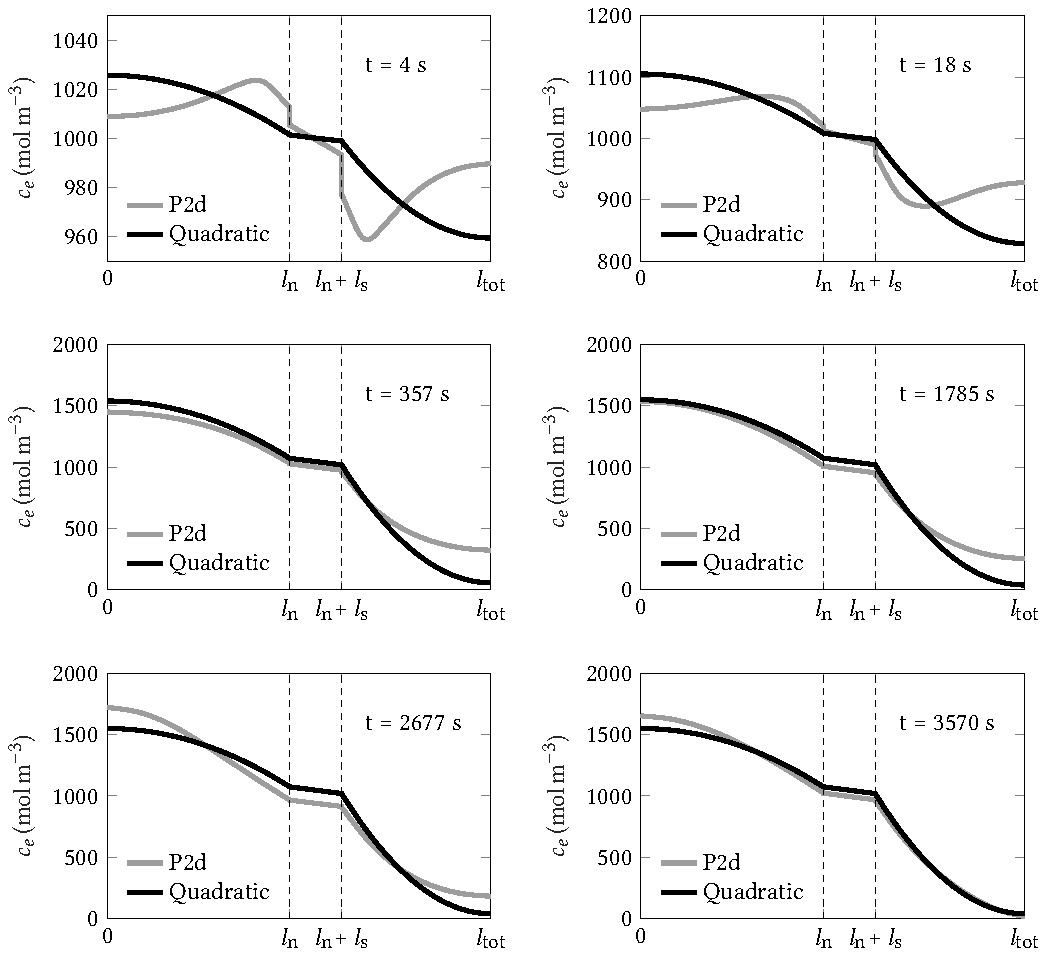
\includegraphics[width=\textwidth]{4/figures/quadratic_ce_approx_spatial_1C.pdf}
    \caption[Spatial distribution of electrolyte concentration for 1C
    discharge]{Spatial distribution of ionic concentration in electrolyte along
        cell thickness at various snapshots of time for a 1C discharge. The
        concentration profile obtained from simulating the \glsfmtshort{p2d}
        model is used as the reference. The performance of the quadratic model
        is quite poor during the initial transient duration, but improves over
    time as a quasi-steady state is reached.}
        \label{fig:spatialionicconc1C}
\end{figure}

\Cref{fig:spatialionicconc1C} shows  the spatial distribution of  \ch{Li^+} ions
in electrolyte  along the  thickness of  the cell at  various snapshots  of time
obtained by simulation  of the \gls{p2d} and the  quadratic approximation models
using a  1C discharge current. The  \gls{p2d} model's response is  considered as
the reference benchmark.  During the initial transient  phase, the concentration
profile within each electrode region exhibits a characteristic inflection point.
During this phase,  the concentration profile computed by  the parabolic profile
exhibits  a  large deviation  in  terms  of  percentage  error at  each  spatial
location. However, with the passage of time, as a \gls{qss} is established, this
inflection point flattens out, and the quadratic approximation becomes closer to
the  true  concentration value  at  each  spatial  location. Similar  trends  in
behaviour is  exhibited for discharge and  charging at higher C-rates  and these
results are  therefore omitted here  in the  interest of keeping  the discussion
succinct.







% -*- root: ../main.tex -*-
%!TEX root = ../main.tex
% this file is called up by main.tex
% content in this file will be fed into the main document
% vim:textwidth=80 fo=cqt

Having performed a  comprehensive analysis of the state of  the art in \gls{spm}
modelling, this section presents the  author's unique contribution to the field.
Firstly, the  scope of the  contribution is identified. The  methodology adopted
and corresponding results are presented thereafter.

\subsection{Scope and motivation}\label{subsec:scopenewelectrolyte}

This subsection is intended as a capstone summary helping to briefly recount the
discussion so far  and to provide a  context for the author's work  in the wider
realm  of the  \gls{spm}  modelling art.  In  the same  vein  as the  discussion
in~\cref{sec:electrolyteinclusion}, the scope of the proposed enhancement to the
\gls{spm} concerns entirely  with improving the electrolyte subsystem  as it has
already been established in~\cref{subsec:simresultsbasicspm} that the simplified
representation of  the solid-phase subsystem  through a fourth  order polynomial
approximation method  for diffusion of  \ch{Li^0} in  the solid particle,  is of
sufficiently high accuracy.

Inspecting the  electrolyte domain,  the electrolyte  overpotential contribution
to  terminal  voltage   consists  of  a  diffusion   overpotential  in  addition
to   the  time-dependent   ohmic  losses   that  originates   from  differential
concentration  gradients  that  is   indirectly  dependent  upon  concentration.
Hence,  accurate  determination  of   spatio-temporal  concentration  takes  the
centre  stage.  For   the  computation  of  overpotential   in  the  electrolyte
phase,~\cref{eq:electrolytepdwithce}  proposed  by  Prada~\etal~\cite{Prada2012}
may be used.

There exists a  subtle detail in the  use of~\cref{eq:electrolytepdwithce} which
is discussed here upfront before proceeding  ahead to the refined context of the
author's  work.  The  intrinsic  conductivity  of  electrolyte,  $\kappa$  is  a
function of  the ionic concentration  (refer~\cref{subsec:basicspmsimsetup}). If
the ionic  concentration at  the corresponding current  collectors are  used for
$\kappa_\text{neg}$  and  $\kappa_\text{pos}$, this  would  lead  to a  lopsided
computation of the overpotential in electrolyte. Furthermore, under this scheme,
the computation of electrolyte conductivity shall be rendered ambiguous since it
is unclear which  separator interface shall be chosen for  the separator's ionic
concentration. Although this  has not been discussed clearly  in literature, the
author  of this  thesis chose  to use  the mean  concentration within  each cell
region, defined as
\begin{equation}
    \mean{c}_{\text{e},j}(t) = \frac{1}{l_j}\int_0^{l_j} c_{\text{e}_j}(z,t)\, dz = \frac{Q_{\text{e}_j}(t)}{\varepsilon_j l_j}
\end{equation}
although other measures  of central tendency might be equally  valid. Hence, the
results of this section have the associated variability in them depending on how
the electrolyte concentration computations are  used in evaluating the intrinsic
conductivity of electrolyte.

As  the  ionic  concentration  has  both  a  direct  and  indirect  contribution
in~\cref{eq:electrolytepdwithce}, its spatio-temporal  computation is a critical
aspect. As discussed  in~\cref{sec:quadraticapprox}, the quadratic approximation
is a widely used spatio-temporal model for electrolyte concentration which makes
the best  use of available physical  constraints. As established in  the results
of~\cref{subsec:quadraticsimresultsanalysis}, while  the spatial  performance of
the quadratic approximation approach is acceptable, its time-domain performance,
particularly at the crucial current collector locations is mediocre at best.

Thus,   the  \emph{scope}   of  the   author's  work   is  to   obtain  suitable
alternate   expressions   for   improving  the   computation   of   \textbf{time
evolution}  of  the electrolyte  concentration  whilst  retaining the  quadratic
approximation   approach   for  describing   its   spatial   profile.  Such   an
approach  is motivated  by  the  keen observation  that  the baseline  quadratic
approximation  model  has  a  natural  `pause'  in  its  model  description.  To
clarify,~\crefrange{eq:cecontinuitynegsep}{eq:Qepbyintegration}  form a  tightly
coupled set of  seven linear equations in seven unknowns.  The time evolution of
$Q_{\text{e}_j}$  are described  through  a system  of  first order  \glspl{ode}
given by~\crefrange{eq:negliionmolesquadratic}{eq:posliionmolesquadratic}.  In a
practical  implementation,  these  \glspl{ode}  are solved  independently  in  a
decoupled  manner,\ie{}  by using  the  coefficients  obtained from  the  linear
system of~\crefrange{eq:cecontinuitynegsep}{eq:Qepbyintegration} in the previous
time-step. The  author's hypothesis is that  by taking advantage of  the natural
break  in the  operational  sequence which  involves  two separate  computations
between  two independent  subsystems (for  all practical  purposes), it  must be
possible  to  replace  the  underperforming time-evolution  equations  from  the
baseline quadratic approximation with a superior alternate model.

\subsection{Methodology --- System identification}

This section presents the methodology adopted in obtaining an improved model for
the rate of evolution  of overall moles per unit area of  \ch{Li^+} ions in each
of the three regions of the cell.

\subsubsection*{Background}\label{subsubsec:sysidbackground}

This  section presents  the  background and  thought  process in  systematically
arriving  at  the  choice of  the  methodology  that  was  adopted for  the  new
time-evolution model of the electrolyte concentration.

Based  upon the  experience  gained  in dealing  with  the literature  presented
in~\cref{sec:electrolyteinclusion}, it is  the author's view that,  owing to the
complex behaviour of electrolyte, a  naive top-down approach \ie{} including all
the physics upfront  followed by a systematic simplification, might  result in a
model that is  mathematically intractable for adoption in  an embedded \gls{bms}
environment.  The baseline  quadratic  approximation method  has  proven that  a
bottom-up  approach, \ie{}  pre-assuming a  simplified structure  for the  final
model  and adapting  its coefficients  to physical  constraints yields  a viable
candidate for inclusion in the conventional \gls{spm}.

Upon  a   closer  examination   of  the  rubrics   of  the   baseline  quadratic
approximation  model, it  comes  to  light that  the  natural `pause'  discussed
towards  the  end  of~\cref{subsec:scopenewelectrolyte}  permeates  to  a  level
more  than  merely  having  to  operate  sequentially  on  two  pseudo-decoupled
subsystems  --- it  goes to  the extent  of rendering  the operating  philosophy
of  fitting  physical  equations  semi-void.   To  clarify  this  statement  and
to  substantiate   the  claim,  while  there   is  no  doubt  that   the  linear
algebraic   equations  of~\crefrange{eq:cecontinuitynegsep}{eq:Qepbyintegration}
do    incorporate    physical    principles   from    the    \gls{dfn}    model,
the     same     does     not      hold     true     for     the     \glspl{ode}
of~\crefrange{eq:negliionmolesquadratic}{eq:posliionmolesquadratic}.   In  fact,
all   the   boundary   conditions   from   the   \gls{dfn}   model   have   been
exhausted   by  this   stage  (refer~\cref{subsec:quadraticsimresultsanalysis}).
Although~\crefrange{eq:negliionmolesgen}{eq:posliionmolesgen}     are    derived
from     the      \gls{dfn}     model,      the     coefficients      of     the
diffusivities   in    the   \gls{rhs}   of    the   next   set    of   equations
\ie{}~\crefrange{eq:negliionmolesquadratic}{eq:posliionmolesquadratic},   merely
involve  substitutions  of the  spatial  derivatives  of the  assumed  quadratic
expression.

Herein lies the weakness of the  baseline quadratic approach. Unlike the spatial
algebraic equations, which are tightly bound by the continuity and flux boundary
conditions at the  separator interfaces, there is no equality  constraint on the
spatial  derivative, which  is free  to grow  or shrink  without any  explicitly
imposed  bounds.  The  onus  of  being accurate  is  therefore  on  the  spatial
derivative evaluation which in-turn depends  on the correctness of the quadratic
functions  (\crefrange{eq:cenquadreduced}{eq:cepquadreduced}) themselves.  It is
not feasible to quantify the magnitude of error introduced in the time-evolution
of concentration  given a small-signal  perturbation in the coefficients  of the
quadratic spatial  computation,\ie{} the implicit  coupling between them  is not
transparent. Since the quadratic approximation itself is not perfect, \ie{} does
not capture the  spatial gradient \emph{exactly} as the \gls{p2d}  model as seen
in~\cref{fig:spatialionicconc1C}, the internal coupling of coefficients leads to
errors in time-evolution computation.

The author's  approach is to  therefore break this detrimental  coupling between
spatial  derivative of  concentration  and its  temporal evolution  counterpart.
Inspired by the fact that the  quadratic approximation model had almost achieved
the desired goals with
\begin{enumerate}[label=\emph{\alph*})]
    \item a bottoms-up approach, \ie{} assuming some model structure apriori, and
    \item not bound by any physical considerations due to the exhaustion of governing equations
\end{enumerate}
have led  the author  to broach  a modelling concept  that exhibit  these common
traits,  yet  of  a  completely  different nature  and  hitherto  unexplored  in
physics-based  battery  modelling  in   general  and  electrolyte  modelling  in
particular --- \emph{black-box system identification}.

\subsubsection*{Brief introduction to system identification}\label{subsubsec:introsysid}

An in-depth  coverage of the topic  of system identification is  well beyond the
scope of  this thesis.  However, keeping  in mind the  interests of  the battery
modelling community  who might not be  familiar with this subject  area, a brief
overview of the core ideas that  are essential for tackling the specific problem
at hand, is presented. For readers  further interested in this topic, the author
suggests the textbook by  Ljung~\cite{Ljung1999} for a comprehensive theoretical
treatment of the foundation topics in system identification.

System identification aims  to provide a mathematical model  of the input-output
mapping  of  a system\footnote{The  precise  definition  of what  constitutes  a
`system' is detailed  in Ljung's textbook. However, for  all practical purposes,
in this  thesis the word `system'  stands for any unknown  entity whose terminal
behavioural model  is being  sought for ---  primarily from  input-output data.}
under consideration. The three categories of system identification are:


\begin{enumdescriptnum}[leftmargin=!,itemsep=1ex,labelwidth=\widthof{$\symbf{\text{brugg}_j}\ \scriptstyle (\times 3)$abc}
    ,partopsep=0pt
    ,topsep=0pt
    ]

\item[White box] wherein underlying physical equations are completely known. The
numerical value  of coefficients of  governing equations are to  be parametrised
from input-output data.

\item[Black box]  wherein no  governing equations are  available for  the system
under  consideration. The  model formulation  is facilitated  by a  rich set  of
system theory  which proceeds by exciting  the system with input  waveforms with
certain desirable  properties and correlating characteristics  from the response
in order  to draw  conclusions about viable  mathematical structures  capable of
emulating  the  terminal  behaviour  of the  system  under  generalised  inputs.
Black  box system  identification was  employed for  the specific  problem under
consideration and hence all future descriptions will pertain to this class.

\item[Grey box] is a hybrid of the  two approaches wherein a part of the model's
governing  physics is  known a  priori, \eg{}  the structure  of a  well-defined
subsystem  that is  part  of a  large,  complex  system may  be  known ahead  of
time,  where the  task  is  to characterise  the  full  system. Grey-box  system
identification tasks can  often be reduced to a single  sub-problem of black-box
system  identification  by  removal  of  the known  physics  and  tackling  them
separately.

\end{enumdescriptnum}

\subsubsection*{Overview of black-box system identification}\label{subsubsec:introblackboxsysid}
Black-box system identification techniques can be broadly classified into ---
\begin{enumerate*}[label=\emph{\alph*})]
     \item non-parametric methods, and
     \item parametric methods.
 \end{enumerate*}

Non-parametric methods do not seek  a pre-assumed mathematical structure for the
system. They  aim to  directly estimate  the very  kernel of  what characterises
every system \viz{}  the Markov parameters in the time-domain  and the \gls{frf}
in the frequency domain, thereby requiring \emph{infinite} number of data points
for  their representation.  Major non-parametric  system identification  methods
include:
\begin{itemize}[topsep=0pt]
    \item Identification in time domain
        \begin{itemize}

            \item Direct  estimation of the system's  Markov parameters through
                statistical correlation of its response to an unit-pulse input

        \end{itemize}
    \item Identification in frequency domain,  \ie{} of the \gls{frf}
        \begin{enumerate}

            \item   Direct   estimation    through   input-output   statistical
                cross-correlation

            \item  \gls{etfe} using \glspl{dft} of input and output sequences

            \item  Smoothed periodogram estimates using Welch's method

            \item  Blackman-Tukey  estimation   method  using  standard  filter
                windows  in digital  signal processing  (such as  Hamming, Hanning,
                Bartlett, Boxcar etc.)

        \end{enumerate}
\end{itemize}

Parametric  methods  aim  to  fit  specific input-output  data  to  some  family
of  well-known  mathematical  constructs  that  generalise  well  to  a  variety
of  inputs.  It  is  important  to recognise  that,  in  contrast  to  white-box
system identification, the salient coefficients/properties of these mathematical
structures do  not, in any way  correspond to physical properties  of the system
under consideration. Major parametric system identification methods are:
\begin{itemize}
    \item Transfer-function based frequency domain model structures
        \begin{enumerate}
            \item \gls{oe} model
            \item \gls{arx} model
            \item \gls{armax} model
            \item Box-Jenkins (BJ) model
        \end{enumerate}
    \item State-space time-domain model structures
        \begin{enumerate}
            \item Ho-Kalman realisation
            \item \gls{era} realisation
            \item Deterministic and stochastic \emph{subspace} structures
        \end{enumerate}
\end{itemize}

Among  these  system  identification  methods, the  non-parametric  methods  are
immediately  ruled  out   for  applying  to  the  task  at   hand.  As  outlined
in~\cref{subsubsec:sysidbackground},  the author  is  inspired by  the trait  of
having  a  pre-assumed  model  structure that  brought  the  baseline  quadratic
approximation closer to a successful  realisation. The non-parametric methods do
not conform to this philosophy.  Furthermore, the requirement of infinite number
of data  samples in order to  fully quantify the system  dampens its feasibility
for implementation  in resource constrained  environments. The author is  of the
opinion that resorting  to truncation of the characteristic  sequence shall only
yield a sub-optimal solution.

While  parametric state-space  identification is  a feasible  alternative, these
methodologies  are   tedious  and   error-prone.  For  instance,   applying  the
Ho-Kalman  algorithm requires  construction  of  Block-Hankel matrices  followed
by  a  \gls{svd} operation.  The  \gls{era}  brings  with  an identical  set  of
operations  of  the  Ho-Kalman  procedure, except  that  certain  random  blocks
in  the  Hankel   matrices  are  chosen  at  random  for   deletion  for  better
estimates  in  low \gls{snr}  environments  and  for capturing  slowly  decaying
phenomena  with long  time constants.  The subspace  methods are  mathematically
involved,  requiring  a  profound  understanding of  projections  to  orthogonal
subspaces  from linear  algebra.  The system  under  consideration is  presented
in~\cref{subsubsec:sysidplantmodel}.  It   is  composed  of   three  independent
\gls{siso}  subsystems.  The  complexity-performance  trade-off  in  state-space
identification  is  achieved only  when  dealing  with \gls{mimo}  systems  that
suggest strong cross-coupling among its internal  states or at least some degree
of  coupling among  the various  inputs  and outputs.  Furthermore, the  impulse
responses of  the system under  consideration does not  have long tails  and are
characterised by relatively short time constants. Owing to these reasons, it was
decided that state space identification methods shall not be adopted here.

Owing to a  cornucopia of well-established technical  know-how readily available
in the systems  engineers toolkit, transfer function based  model structures are
naturally amenable for  control oriented applications. However,  there exists an
apparent  discrepancy  to its  usage  that  must  be addressed  first.  Transfer
function  methods are  a frequency  domain  technique and  hence, the  resulting
model  descriptions have  mathematical structures  radically different  from the
time-domain model equations of the  conventional \gls{spm} within which they are
to be  embedded. This conundrum  is resolved  by closely inspecting  the model's
scope and its tractability for conversion to time domain as explained next.

It is worth remembering that, as per~\cref{subsec:freqdomainroms}, all frequency
domain model groups were considered as  out of scope of this thesis specifically
due  to  the   overhead  of  conversion  from  frequency  to   time  domain  for
implementation  and other  associated difficulties  for the  \glspl{rom} of  the
\emph{entire cell}.  The blanket  exclusion nature  of this  statement is  to be
revisited considering  the specific scope  of the problem  at hand. The  body of
literature  on  frequency  domain \glspl{rom}  discuss  obtaining  physics-based
transcendental  transfer functions  for  all electrochemical  quantities of  the
coupled  \gls{pdae} system  of~\cref{tbl:dfneqns} through  a top-down  approach.
However, the frequency  domain system identification methods  are concerned with
obtaining standard  rational transfer  functions for a  system of  much narrowed
scope, \ie{}  for the  time-evolution subsystem,  through a  bottom-up approach.
Such  rational transfer  functions are  to obtained  for \gls{siso}  systems for
which  an approximation-free  effortless  conversion exists  based on  classical
control  theory and  is presented  in~\cref{subsubsec:sysidplantmodel}. In  view
of  their  simplicity  and  familiarity, and  after  successfully  circumventing
their  only apparent  impediment  to adoption,  transfer  function based  system
identification was  chosen for  tackling the  problem at  hand and  is presented
next.


\subsubsection*{Transfer function identification of electrolyte time-evolution subsystem}\label{subsubsec:sysidplantmodel}

\Crefrange{eq:negliionmolesquadratic}{eq:posliionmolesquadratic} of the baseline
quadratic  approximation  model for  electrolyte  concentration  pertain to  the
time-evolution of the overall number  of moles of \ch{Li^+}, $Q_{\text{e,}j}$ in
each  of  the  three  regions  of the  cell  and  are  first  order~\glspl{ode}.
Through system  identification, we  desire to obtain  the two  rational transfer
functions  of  $Q_\text{e,neg}$  and  $Q_\text{e,pos}$ to  applied  current  $I$
in  the  frequency  domain,  \ie{} we  seek  $\frac{Q_\text{e,n}(s)}{I(s)}$  and
$\frac{Q_\text{e,p}(s)}{I(s)}$. Based on the \gls{dfn} model, the total moles of
\ch{Li^+} per  unit area in the  separator, $Q_\text{e,s}$ is not  a function of
the exogenous applied current and the baseline quadratic approximation \gls{ode}
is retained for computing its time-evolution.

In order  to successfully apply  any system identification technique,  the input
signal must be carefully  designed to be persistently exciting~\cite{Ljung1999}.
Narendra and Annaswamy~\cite{Narendra1984,Narendra1987}  were among the earliest
researchers  to provide  a detailed  treatment  of the  desirable properties  of
persistent excitation and their implication to the quality of the identification
output. A  practical method to achieve  persistent excitation is to  subject the
system under  consideration to  a sequence  of well-characterised  input signals
that  are  capable of  exciting  its  hypothesised  modes.  The author  of  this
thesis  chose  to  use  the  data-quality guidance  provided  by  the  Mathworks
Inc.~\cite{mathworkssysid}\ for this task  and performed an iterative refinement
until the identification procedure resulted in a generalisable model.


In order to apply the transfer function identification techniques, linearity and
time-invariance of the underlying system must be established.


\printglossary[type=acronym]
\cleardoublepage

\begin{appendices} % Using appendices environment for more functionality
    \crefalias{chapter}{appchap}
    % -*- root: ../main.tex -*-
%!TEX root = ../main.tex
% ******************************* Thesis Appendix A ****************************
\chapter{Full Listing of Program Codes}

dummy cts time \label{sc:ctstimespm}

dummy disc time\label{sc:disctimespm}
% \tikzexternaldisable
% \matlabcodelisting[MATLAB code for simulation of continuous time \protect{\gls{spm}}]{Appendix1/matlab_codes/cts_time_spm_simulation.m}{sc:ctstimespm}
% \tikzexternalenable
% graphviz doc in appendix, toolbox, directory listing etc.

\end{appendices}

\backmatter

\begin{footnotesize} % tiny(5) < scriptsize(7) < footnotesize(8) < small (9)
    \renewcommand{\bibname}{References} % changes the header; default: Bibliography
    % add bib to toc
    \cleardoublepage
    \phantomsection
    \addcontentsline{toc}{chapter}{\bibname}
    \printbibliography
\end{footnotesize}
\batchmode
\end{document}
